\section{Introduction}

\subsection{Background}
\begin{frame}
    \frametitle{The Clean Energy Transition}
    Our changing climate and additional demand drivers from data 
    centers and \gls{ai} require a just transition from fossil 
    fuels to clean energy.
\end{frame}

\begin{frame}
    \frametitle{Three tenets of justice}
    \begin{figure}
        \centering
        % \resizebox{0.7\columnwidth}{!}{
            \begin{tikzpicture}
                \begin{scope}[blend group = soft light]
                    % \fill[red!30!white]   ( 90:1.2) circle (2);
                    \fill[illiniorange]   ( 90:1.2) circle (2);
                    % \fill[green!30!white] (210:1.2) circle (2);
                    \fill[illiniorange] (210:1.2) circle (2);
                    % \fill[blue!30!white]  (330:1.2) circle (2);
                    \fill[illiniorange]  (330:1.2) circle (2);
                \end{scope}
                \node at ( 90:2)    {Recognition}; 
                \node at ( 210:2) {Distribution}; 
                \node at ( 330:2)   {Procedural}; 
                \node[font=\Large] {\textcolor{black}{Justice}};
              \end{tikzpicture}

        % }
        \caption{Three aspects of justice \cite{schlosberg_1_2007}.}
    \end{figure}
\end{frame}

\begin{frame}
    \frametitle{\glspl{esom}}
    \Glspl{esom} are a class of tools designed to 
    optimize this transition.
    \\
    % (Provide examples?)

    They will become more important with more \gls{vre}
    and more volatile weather.
    \\\\
    \textit{But they have at least two big flaws}.
    \begin{enumerate}[<+->]
        \item All current \glspl{esom} optimize a single objective --- cost.
        \item \glspl{esom} struggle to model the ``human dimension'' thereby
        limiting their ability to address justice \cite{pfenninger_energy_2014}.
    \end{enumerate}
\end{frame}

\subsection{Introducing \gls{osier}}
\begin{frame}
    \frametitle{\gls{osier}}
    I developed \gls{osier} to fill these gaps by \cite{dotson_osier_2024}
    \begin{enumerate}
        \item optimizing multi- and many-objective problems,
        \item allowing user-defined objectives.
    \end{enumerate}
    
    \begin{figure}
        \centering
        \resizebox{0.95\columnwidth}{!}{%% Creator: Matplotlib, PGF backend
%%
%% To include the figure in your LaTeX document, write
%%   \input{<filename>.pgf}
%%
%% Make sure the required packages are loaded in your preamble
%%   \usepackage{pgf}
%%
%% Also ensure that all the required font packages are loaded; for instance,
%% the lmodern package is sometimes necessary when using math font.
%%   \usepackage{lmodern}
%%
%% Figures using additional raster images can only be included by \input if
%% they are in the same directory as the main LaTeX file. For loading figures
%% from other directories you can use the `import` package
%%   \usepackage{import}
%%
%% and then include the figures with
%%   \import{<path to file>}{<filename>.pgf}
%%
%% Matplotlib used the following preamble
%%   \def\mathdefault#1{#1}
%%   \everymath=\expandafter{\the\everymath\displaystyle}
%%   \IfFileExists{scrextend.sty}{
%%     \usepackage[fontsize=10.000000pt]{scrextend}
%%   }{
%%     \renewcommand{\normalsize}{\fontsize{10.000000}{12.000000}\selectfont}
%%     \normalsize
%%   }
%%   
%%   \makeatletter\@ifpackageloaded{underscore}{}{\usepackage[strings]{underscore}}\makeatother
%%
\begingroup%
\makeatletter%
\begin{pgfpicture}%
\pgfpathrectangle{\pgfpointorigin}{\pgfqpoint{6.600000in}{5.000000in}}%
\pgfusepath{use as bounding box, clip}%
\begin{pgfscope}%
\pgfsetbuttcap%
\pgfsetmiterjoin%
\definecolor{currentfill}{rgb}{1.000000,1.000000,1.000000}%
\pgfsetfillcolor{currentfill}%
\pgfsetlinewidth{0.000000pt}%
\definecolor{currentstroke}{rgb}{0.000000,0.000000,0.000000}%
\pgfsetstrokecolor{currentstroke}%
\pgfsetdash{}{0pt}%
\pgfpathmoveto{\pgfqpoint{0.000000in}{0.000000in}}%
\pgfpathlineto{\pgfqpoint{6.600000in}{0.000000in}}%
\pgfpathlineto{\pgfqpoint{6.600000in}{5.000000in}}%
\pgfpathlineto{\pgfqpoint{0.000000in}{5.000000in}}%
\pgfpathlineto{\pgfqpoint{0.000000in}{0.000000in}}%
\pgfpathclose%
\pgfusepath{fill}%
\end{pgfscope}%
\end{pgfpicture}%
\makeatother%
\endgroup%
}
        \caption{Objective space for a four-objective problem.}
        \label{fig:4-obj-space}
    \end{figure}
\end{frame}

\begin{frame}
    \frametitle{How \gls{osier} Works}

    \begin{figure}
        \centering
        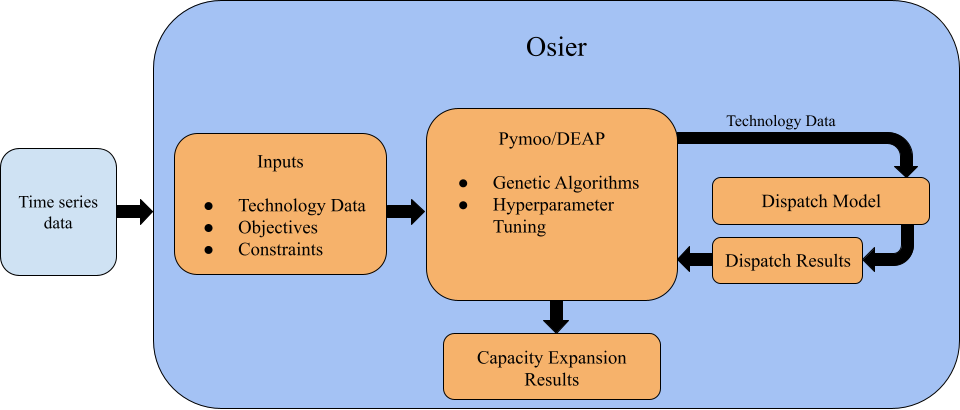
\includegraphics[width=\columnwidth]{../docs/figures/03_osier_chapter/osier_flow.png}
        \caption{Flow of data into and within \gls{osier}}
        \label{fig:osier-flow-1}
    \end{figure}
    % [Show the data flow diagram]

    % Osier works by leveraging genetic algorithsm... 
\end{frame}

\begin{frame}
    \frametitle{Pareto Fronts}
    \begin{figure}
        \centering
        \resizebox{0.75\columnwidth}{!}{%% Creator: Matplotlib, PGF backend
%%
%% To include the figure in your LaTeX document, write
%%   \input{<filename>.pgf}
%%
%% Make sure the required packages are loaded in your preamble
%%   \usepackage{pgf}
%%
%% Also ensure that all the required font packages are loaded; for instance,
%% the lmodern package is sometimes necessary when using math font.
%%   \usepackage{lmodern}
%%
%% Figures using additional raster images can only be included by \input if
%% they are in the same directory as the main LaTeX file. For loading figures
%% from other directories you can use the `import` package
%%   \usepackage{import}
%%
%% and then include the figures with
%%   \import{<path to file>}{<filename>.pgf}
%%
%% Matplotlib used the following preamble
%%   \def\mathdefault#1{#1}
%%   \everymath=\expandafter{\the\everymath\displaystyle}
%%   \IfFileExists{scrextend.sty}{
%%     \usepackage[fontsize=10.000000pt]{scrextend}
%%   }{
%%     \renewcommand{\normalsize}{\fontsize{10.000000}{12.000000}\selectfont}
%%     \normalsize
%%   }
%%   
%%   \makeatletter\@ifpackageloaded{underscore}{}{\usepackage[strings]{underscore}}\makeatother
%%
\begingroup%
\makeatletter%
\begin{pgfpicture}%
\pgfpathrectangle{\pgfpointorigin}{\pgfqpoint{6.869444in}{5.322237in}}%
\pgfusepath{use as bounding box, clip}%
\begin{pgfscope}%
\pgfsetbuttcap%
\pgfsetmiterjoin%
\definecolor{currentfill}{rgb}{1.000000,1.000000,1.000000}%
\pgfsetfillcolor{currentfill}%
\pgfsetlinewidth{0.000000pt}%
\definecolor{currentstroke}{rgb}{0.000000,0.000000,0.000000}%
\pgfsetstrokecolor{currentstroke}%
\pgfsetdash{}{0pt}%
\pgfpathmoveto{\pgfqpoint{0.000000in}{0.000000in}}%
\pgfpathlineto{\pgfqpoint{6.869444in}{0.000000in}}%
\pgfpathlineto{\pgfqpoint{6.869444in}{5.322237in}}%
\pgfpathlineto{\pgfqpoint{0.000000in}{5.322237in}}%
\pgfpathlineto{\pgfqpoint{0.000000in}{0.000000in}}%
\pgfpathclose%
\pgfusepath{fill}%
\end{pgfscope}%
\begin{pgfscope}%
\pgfsetbuttcap%
\pgfsetmiterjoin%
\definecolor{currentfill}{rgb}{1.000000,1.000000,1.000000}%
\pgfsetfillcolor{currentfill}%
\pgfsetlinewidth{0.000000pt}%
\definecolor{currentstroke}{rgb}{0.000000,0.000000,0.000000}%
\pgfsetstrokecolor{currentstroke}%
\pgfsetstrokeopacity{0.000000}%
\pgfsetdash{}{0pt}%
\pgfpathmoveto{\pgfqpoint{0.569444in}{0.554012in}}%
\pgfpathlineto{\pgfqpoint{6.769444in}{0.554012in}}%
\pgfpathlineto{\pgfqpoint{6.769444in}{5.174012in}}%
\pgfpathlineto{\pgfqpoint{0.569444in}{5.174012in}}%
\pgfpathlineto{\pgfqpoint{0.569444in}{0.554012in}}%
\pgfpathclose%
\pgfusepath{fill}%
\end{pgfscope}%
\begin{pgfscope}%
\pgfpathrectangle{\pgfqpoint{0.569444in}{0.554012in}}{\pgfqpoint{6.200000in}{4.620000in}}%
\pgfusepath{clip}%
\pgfsetbuttcap%
\pgfsetroundjoin%
\pgfsetlinewidth{1.003750pt}%
\definecolor{currentstroke}{rgb}{1.000000,0.000000,0.000000}%
\pgfsetstrokecolor{currentstroke}%
\pgfsetdash{}{0pt}%
\pgfpathmoveto{\pgfqpoint{0.569444in}{5.132345in}}%
\pgfpathcurveto{\pgfqpoint{0.580495in}{5.132345in}}{\pgfqpoint{0.591094in}{5.136735in}}{\pgfqpoint{0.598907in}{5.144549in}}%
\pgfpathcurveto{\pgfqpoint{0.606721in}{5.152363in}}{\pgfqpoint{0.611111in}{5.162962in}}{\pgfqpoint{0.611111in}{5.174012in}}%
\pgfpathcurveto{\pgfqpoint{0.611111in}{5.185062in}}{\pgfqpoint{0.606721in}{5.195661in}}{\pgfqpoint{0.598907in}{5.203475in}}%
\pgfpathcurveto{\pgfqpoint{0.591094in}{5.211288in}}{\pgfqpoint{0.580495in}{5.215678in}}{\pgfqpoint{0.569444in}{5.215678in}}%
\pgfpathcurveto{\pgfqpoint{0.558394in}{5.215678in}}{\pgfqpoint{0.547795in}{5.211288in}}{\pgfqpoint{0.539982in}{5.203475in}}%
\pgfpathcurveto{\pgfqpoint{0.532168in}{5.195661in}}{\pgfqpoint{0.527778in}{5.185062in}}{\pgfqpoint{0.527778in}{5.174012in}}%
\pgfpathcurveto{\pgfqpoint{0.527778in}{5.162962in}}{\pgfqpoint{0.532168in}{5.152363in}}{\pgfqpoint{0.539982in}{5.144549in}}%
\pgfpathcurveto{\pgfqpoint{0.547795in}{5.136735in}}{\pgfqpoint{0.558394in}{5.132345in}}{\pgfqpoint{0.569444in}{5.132345in}}%
\pgfpathlineto{\pgfqpoint{0.569444in}{5.132345in}}%
\pgfpathclose%
\pgfusepath{stroke}%
\end{pgfscope}%
\begin{pgfscope}%
\pgfpathrectangle{\pgfqpoint{0.569444in}{0.554012in}}{\pgfqpoint{6.200000in}{4.620000in}}%
\pgfusepath{clip}%
\pgfsetbuttcap%
\pgfsetroundjoin%
\pgfsetlinewidth{1.003750pt}%
\definecolor{currentstroke}{rgb}{1.000000,0.000000,0.000000}%
\pgfsetstrokecolor{currentstroke}%
\pgfsetdash{}{0pt}%
\pgfpathmoveto{\pgfqpoint{0.570375in}{5.031408in}}%
\pgfpathcurveto{\pgfqpoint{0.581425in}{5.031408in}}{\pgfqpoint{0.592024in}{5.035798in}}{\pgfqpoint{0.599838in}{5.043612in}}%
\pgfpathcurveto{\pgfqpoint{0.607651in}{5.051426in}}{\pgfqpoint{0.612041in}{5.062025in}}{\pgfqpoint{0.612041in}{5.073075in}}%
\pgfpathcurveto{\pgfqpoint{0.612041in}{5.084125in}}{\pgfqpoint{0.607651in}{5.094724in}}{\pgfqpoint{0.599838in}{5.102538in}}%
\pgfpathcurveto{\pgfqpoint{0.592024in}{5.110351in}}{\pgfqpoint{0.581425in}{5.114742in}}{\pgfqpoint{0.570375in}{5.114742in}}%
\pgfpathcurveto{\pgfqpoint{0.559325in}{5.114742in}}{\pgfqpoint{0.548726in}{5.110351in}}{\pgfqpoint{0.540912in}{5.102538in}}%
\pgfpathcurveto{\pgfqpoint{0.533098in}{5.094724in}}{\pgfqpoint{0.528708in}{5.084125in}}{\pgfqpoint{0.528708in}{5.073075in}}%
\pgfpathcurveto{\pgfqpoint{0.528708in}{5.062025in}}{\pgfqpoint{0.533098in}{5.051426in}}{\pgfqpoint{0.540912in}{5.043612in}}%
\pgfpathcurveto{\pgfqpoint{0.548726in}{5.035798in}}{\pgfqpoint{0.559325in}{5.031408in}}{\pgfqpoint{0.570375in}{5.031408in}}%
\pgfpathlineto{\pgfqpoint{0.570375in}{5.031408in}}%
\pgfpathclose%
\pgfusepath{stroke}%
\end{pgfscope}%
\begin{pgfscope}%
\pgfpathrectangle{\pgfqpoint{0.569444in}{0.554012in}}{\pgfqpoint{6.200000in}{4.620000in}}%
\pgfusepath{clip}%
\pgfsetbuttcap%
\pgfsetroundjoin%
\pgfsetlinewidth{1.003750pt}%
\definecolor{currentstroke}{rgb}{1.000000,0.000000,0.000000}%
\pgfsetstrokecolor{currentstroke}%
\pgfsetdash{}{0pt}%
\pgfpathmoveto{\pgfqpoint{0.573166in}{4.931496in}}%
\pgfpathcurveto{\pgfqpoint{0.584216in}{4.931496in}}{\pgfqpoint{0.594815in}{4.935886in}}{\pgfqpoint{0.602628in}{4.943700in}}%
\pgfpathcurveto{\pgfqpoint{0.610442in}{4.951514in}}{\pgfqpoint{0.614832in}{4.962113in}}{\pgfqpoint{0.614832in}{4.973163in}}%
\pgfpathcurveto{\pgfqpoint{0.614832in}{4.984213in}}{\pgfqpoint{0.610442in}{4.994812in}}{\pgfqpoint{0.602628in}{5.002626in}}%
\pgfpathcurveto{\pgfqpoint{0.594815in}{5.010439in}}{\pgfqpoint{0.584216in}{5.014829in}}{\pgfqpoint{0.573166in}{5.014829in}}%
\pgfpathcurveto{\pgfqpoint{0.562115in}{5.014829in}}{\pgfqpoint{0.551516in}{5.010439in}}{\pgfqpoint{0.543703in}{5.002626in}}%
\pgfpathcurveto{\pgfqpoint{0.535889in}{4.994812in}}{\pgfqpoint{0.531499in}{4.984213in}}{\pgfqpoint{0.531499in}{4.973163in}}%
\pgfpathcurveto{\pgfqpoint{0.531499in}{4.962113in}}{\pgfqpoint{0.535889in}{4.951514in}}{\pgfqpoint{0.543703in}{4.943700in}}%
\pgfpathcurveto{\pgfqpoint{0.551516in}{4.935886in}}{\pgfqpoint{0.562115in}{4.931496in}}{\pgfqpoint{0.573166in}{4.931496in}}%
\pgfpathlineto{\pgfqpoint{0.573166in}{4.931496in}}%
\pgfpathclose%
\pgfusepath{stroke}%
\end{pgfscope}%
\begin{pgfscope}%
\pgfpathrectangle{\pgfqpoint{0.569444in}{0.554012in}}{\pgfqpoint{6.200000in}{4.620000in}}%
\pgfusepath{clip}%
\pgfsetbuttcap%
\pgfsetroundjoin%
\pgfsetlinewidth{1.003750pt}%
\definecolor{currentstroke}{rgb}{1.000000,0.000000,0.000000}%
\pgfsetstrokecolor{currentstroke}%
\pgfsetdash{}{0pt}%
\pgfpathmoveto{\pgfqpoint{0.577817in}{4.832609in}}%
\pgfpathcurveto{\pgfqpoint{0.588867in}{4.832609in}}{\pgfqpoint{0.599466in}{4.836999in}}{\pgfqpoint{0.607280in}{4.844813in}}%
\pgfpathcurveto{\pgfqpoint{0.615093in}{4.852626in}}{\pgfqpoint{0.619484in}{4.863225in}}{\pgfqpoint{0.619484in}{4.874275in}}%
\pgfpathcurveto{\pgfqpoint{0.619484in}{4.885325in}}{\pgfqpoint{0.615093in}{4.895924in}}{\pgfqpoint{0.607280in}{4.903738in}}%
\pgfpathcurveto{\pgfqpoint{0.599466in}{4.911552in}}{\pgfqpoint{0.588867in}{4.915942in}}{\pgfqpoint{0.577817in}{4.915942in}}%
\pgfpathcurveto{\pgfqpoint{0.566767in}{4.915942in}}{\pgfqpoint{0.556168in}{4.911552in}}{\pgfqpoint{0.548354in}{4.903738in}}%
\pgfpathcurveto{\pgfqpoint{0.540541in}{4.895924in}}{\pgfqpoint{0.536150in}{4.885325in}}{\pgfqpoint{0.536150in}{4.874275in}}%
\pgfpathcurveto{\pgfqpoint{0.536150in}{4.863225in}}{\pgfqpoint{0.540541in}{4.852626in}}{\pgfqpoint{0.548354in}{4.844813in}}%
\pgfpathcurveto{\pgfqpoint{0.556168in}{4.836999in}}{\pgfqpoint{0.566767in}{4.832609in}}{\pgfqpoint{0.577817in}{4.832609in}}%
\pgfpathlineto{\pgfqpoint{0.577817in}{4.832609in}}%
\pgfpathclose%
\pgfusepath{stroke}%
\end{pgfscope}%
\begin{pgfscope}%
\pgfpathrectangle{\pgfqpoint{0.569444in}{0.554012in}}{\pgfqpoint{6.200000in}{4.620000in}}%
\pgfusepath{clip}%
\pgfsetbuttcap%
\pgfsetroundjoin%
\pgfsetlinewidth{1.003750pt}%
\definecolor{currentstroke}{rgb}{1.000000,0.000000,0.000000}%
\pgfsetstrokecolor{currentstroke}%
\pgfsetdash{}{0pt}%
\pgfpathmoveto{\pgfqpoint{0.584329in}{4.734746in}}%
\pgfpathcurveto{\pgfqpoint{0.595379in}{4.734746in}}{\pgfqpoint{0.605978in}{4.739136in}}{\pgfqpoint{0.613792in}{4.746950in}}%
\pgfpathcurveto{\pgfqpoint{0.621605in}{4.754763in}}{\pgfqpoint{0.625996in}{4.765362in}}{\pgfqpoint{0.625996in}{4.776413in}}%
\pgfpathcurveto{\pgfqpoint{0.625996in}{4.787463in}}{\pgfqpoint{0.621605in}{4.798062in}}{\pgfqpoint{0.613792in}{4.805875in}}%
\pgfpathcurveto{\pgfqpoint{0.605978in}{4.813689in}}{\pgfqpoint{0.595379in}{4.818079in}}{\pgfqpoint{0.584329in}{4.818079in}}%
\pgfpathcurveto{\pgfqpoint{0.573279in}{4.818079in}}{\pgfqpoint{0.562680in}{4.813689in}}{\pgfqpoint{0.554866in}{4.805875in}}%
\pgfpathcurveto{\pgfqpoint{0.547052in}{4.798062in}}{\pgfqpoint{0.542662in}{4.787463in}}{\pgfqpoint{0.542662in}{4.776413in}}%
\pgfpathcurveto{\pgfqpoint{0.542662in}{4.765362in}}{\pgfqpoint{0.547052in}{4.754763in}}{\pgfqpoint{0.554866in}{4.746950in}}%
\pgfpathcurveto{\pgfqpoint{0.562680in}{4.739136in}}{\pgfqpoint{0.573279in}{4.734746in}}{\pgfqpoint{0.584329in}{4.734746in}}%
\pgfpathlineto{\pgfqpoint{0.584329in}{4.734746in}}%
\pgfpathclose%
\pgfusepath{stroke}%
\end{pgfscope}%
\begin{pgfscope}%
\pgfpathrectangle{\pgfqpoint{0.569444in}{0.554012in}}{\pgfqpoint{6.200000in}{4.620000in}}%
\pgfusepath{clip}%
\pgfsetbuttcap%
\pgfsetroundjoin%
\pgfsetlinewidth{1.003750pt}%
\definecolor{currentstroke}{rgb}{1.000000,0.000000,0.000000}%
\pgfsetstrokecolor{currentstroke}%
\pgfsetdash{}{0pt}%
\pgfpathmoveto{\pgfqpoint{0.592701in}{4.637908in}}%
\pgfpathcurveto{\pgfqpoint{0.603752in}{4.637908in}}{\pgfqpoint{0.614351in}{4.642298in}}{\pgfqpoint{0.622164in}{4.650112in}}%
\pgfpathcurveto{\pgfqpoint{0.629978in}{4.657926in}}{\pgfqpoint{0.634368in}{4.668525in}}{\pgfqpoint{0.634368in}{4.679575in}}%
\pgfpathcurveto{\pgfqpoint{0.634368in}{4.690625in}}{\pgfqpoint{0.629978in}{4.701224in}}{\pgfqpoint{0.622164in}{4.709037in}}%
\pgfpathcurveto{\pgfqpoint{0.614351in}{4.716851in}}{\pgfqpoint{0.603752in}{4.721241in}}{\pgfqpoint{0.592701in}{4.721241in}}%
\pgfpathcurveto{\pgfqpoint{0.581651in}{4.721241in}}{\pgfqpoint{0.571052in}{4.716851in}}{\pgfqpoint{0.563239in}{4.709037in}}%
\pgfpathcurveto{\pgfqpoint{0.555425in}{4.701224in}}{\pgfqpoint{0.551035in}{4.690625in}}{\pgfqpoint{0.551035in}{4.679575in}}%
\pgfpathcurveto{\pgfqpoint{0.551035in}{4.668525in}}{\pgfqpoint{0.555425in}{4.657926in}}{\pgfqpoint{0.563239in}{4.650112in}}%
\pgfpathcurveto{\pgfqpoint{0.571052in}{4.642298in}}{\pgfqpoint{0.581651in}{4.637908in}}{\pgfqpoint{0.592701in}{4.637908in}}%
\pgfpathlineto{\pgfqpoint{0.592701in}{4.637908in}}%
\pgfpathclose%
\pgfusepath{stroke}%
\end{pgfscope}%
\begin{pgfscope}%
\pgfpathrectangle{\pgfqpoint{0.569444in}{0.554012in}}{\pgfqpoint{6.200000in}{4.620000in}}%
\pgfusepath{clip}%
\pgfsetbuttcap%
\pgfsetroundjoin%
\pgfsetlinewidth{1.003750pt}%
\definecolor{currentstroke}{rgb}{1.000000,0.000000,0.000000}%
\pgfsetstrokecolor{currentstroke}%
\pgfsetdash{}{0pt}%
\pgfpathmoveto{\pgfqpoint{0.602934in}{4.542095in}}%
\pgfpathcurveto{\pgfqpoint{0.613985in}{4.542095in}}{\pgfqpoint{0.624584in}{4.546485in}}{\pgfqpoint{0.632397in}{4.554299in}}%
\pgfpathcurveto{\pgfqpoint{0.640211in}{4.562112in}}{\pgfqpoint{0.644601in}{4.572711in}}{\pgfqpoint{0.644601in}{4.583761in}}%
\pgfpathcurveto{\pgfqpoint{0.644601in}{4.594812in}}{\pgfqpoint{0.640211in}{4.605411in}}{\pgfqpoint{0.632397in}{4.613224in}}%
\pgfpathcurveto{\pgfqpoint{0.624584in}{4.621038in}}{\pgfqpoint{0.613985in}{4.625428in}}{\pgfqpoint{0.602934in}{4.625428in}}%
\pgfpathcurveto{\pgfqpoint{0.591884in}{4.625428in}}{\pgfqpoint{0.581285in}{4.621038in}}{\pgfqpoint{0.573472in}{4.613224in}}%
\pgfpathcurveto{\pgfqpoint{0.565658in}{4.605411in}}{\pgfqpoint{0.561268in}{4.594812in}}{\pgfqpoint{0.561268in}{4.583761in}}%
\pgfpathcurveto{\pgfqpoint{0.561268in}{4.572711in}}{\pgfqpoint{0.565658in}{4.562112in}}{\pgfqpoint{0.573472in}{4.554299in}}%
\pgfpathcurveto{\pgfqpoint{0.581285in}{4.546485in}}{\pgfqpoint{0.591884in}{4.542095in}}{\pgfqpoint{0.602934in}{4.542095in}}%
\pgfpathlineto{\pgfqpoint{0.602934in}{4.542095in}}%
\pgfpathclose%
\pgfusepath{stroke}%
\end{pgfscope}%
\begin{pgfscope}%
\pgfpathrectangle{\pgfqpoint{0.569444in}{0.554012in}}{\pgfqpoint{6.200000in}{4.620000in}}%
\pgfusepath{clip}%
\pgfsetbuttcap%
\pgfsetroundjoin%
\pgfsetlinewidth{1.003750pt}%
\definecolor{currentstroke}{rgb}{1.000000,0.000000,0.000000}%
\pgfsetstrokecolor{currentstroke}%
\pgfsetdash{}{0pt}%
\pgfpathmoveto{\pgfqpoint{0.615028in}{4.447306in}}%
\pgfpathcurveto{\pgfqpoint{0.626078in}{4.447306in}}{\pgfqpoint{0.636677in}{4.451697in}}{\pgfqpoint{0.644491in}{4.459510in}}%
\pgfpathcurveto{\pgfqpoint{0.652304in}{4.467324in}}{\pgfqpoint{0.656695in}{4.477923in}}{\pgfqpoint{0.656695in}{4.488973in}}%
\pgfpathcurveto{\pgfqpoint{0.656695in}{4.500023in}}{\pgfqpoint{0.652304in}{4.510622in}}{\pgfqpoint{0.644491in}{4.518436in}}%
\pgfpathcurveto{\pgfqpoint{0.636677in}{4.526249in}}{\pgfqpoint{0.626078in}{4.530640in}}{\pgfqpoint{0.615028in}{4.530640in}}%
\pgfpathcurveto{\pgfqpoint{0.603978in}{4.530640in}}{\pgfqpoint{0.593379in}{4.526249in}}{\pgfqpoint{0.585565in}{4.518436in}}%
\pgfpathcurveto{\pgfqpoint{0.577752in}{4.510622in}}{\pgfqpoint{0.573361in}{4.500023in}}{\pgfqpoint{0.573361in}{4.488973in}}%
\pgfpathcurveto{\pgfqpoint{0.573361in}{4.477923in}}{\pgfqpoint{0.577752in}{4.467324in}}{\pgfqpoint{0.585565in}{4.459510in}}%
\pgfpathcurveto{\pgfqpoint{0.593379in}{4.451697in}}{\pgfqpoint{0.603978in}{4.447306in}}{\pgfqpoint{0.615028in}{4.447306in}}%
\pgfpathlineto{\pgfqpoint{0.615028in}{4.447306in}}%
\pgfpathclose%
\pgfusepath{stroke}%
\end{pgfscope}%
\begin{pgfscope}%
\pgfpathrectangle{\pgfqpoint{0.569444in}{0.554012in}}{\pgfqpoint{6.200000in}{4.620000in}}%
\pgfusepath{clip}%
\pgfsetbuttcap%
\pgfsetroundjoin%
\pgfsetlinewidth{1.003750pt}%
\definecolor{currentstroke}{rgb}{1.000000,0.000000,0.000000}%
\pgfsetstrokecolor{currentstroke}%
\pgfsetdash{}{0pt}%
\pgfpathmoveto{\pgfqpoint{0.628982in}{4.353543in}}%
\pgfpathcurveto{\pgfqpoint{0.640032in}{4.353543in}}{\pgfqpoint{0.650631in}{4.357933in}}{\pgfqpoint{0.658445in}{4.365747in}}%
\pgfpathcurveto{\pgfqpoint{0.666259in}{4.373560in}}{\pgfqpoint{0.670649in}{4.384159in}}{\pgfqpoint{0.670649in}{4.395209in}}%
\pgfpathcurveto{\pgfqpoint{0.670649in}{4.406259in}}{\pgfqpoint{0.666259in}{4.416858in}}{\pgfqpoint{0.658445in}{4.424672in}}%
\pgfpathcurveto{\pgfqpoint{0.650631in}{4.432486in}}{\pgfqpoint{0.640032in}{4.436876in}}{\pgfqpoint{0.628982in}{4.436876in}}%
\pgfpathcurveto{\pgfqpoint{0.617932in}{4.436876in}}{\pgfqpoint{0.607333in}{4.432486in}}{\pgfqpoint{0.599519in}{4.424672in}}%
\pgfpathcurveto{\pgfqpoint{0.591706in}{4.416858in}}{\pgfqpoint{0.587316in}{4.406259in}}{\pgfqpoint{0.587316in}{4.395209in}}%
\pgfpathcurveto{\pgfqpoint{0.587316in}{4.384159in}}{\pgfqpoint{0.591706in}{4.373560in}}{\pgfqpoint{0.599519in}{4.365747in}}%
\pgfpathcurveto{\pgfqpoint{0.607333in}{4.357933in}}{\pgfqpoint{0.617932in}{4.353543in}}{\pgfqpoint{0.628982in}{4.353543in}}%
\pgfpathlineto{\pgfqpoint{0.628982in}{4.353543in}}%
\pgfpathclose%
\pgfusepath{stroke}%
\end{pgfscope}%
\begin{pgfscope}%
\pgfpathrectangle{\pgfqpoint{0.569444in}{0.554012in}}{\pgfqpoint{6.200000in}{4.620000in}}%
\pgfusepath{clip}%
\pgfsetbuttcap%
\pgfsetroundjoin%
\pgfsetlinewidth{1.003750pt}%
\definecolor{currentstroke}{rgb}{1.000000,0.000000,0.000000}%
\pgfsetstrokecolor{currentstroke}%
\pgfsetdash{}{0pt}%
\pgfpathmoveto{\pgfqpoint{0.644797in}{4.260804in}}%
\pgfpathcurveto{\pgfqpoint{0.655847in}{4.260804in}}{\pgfqpoint{0.666446in}{4.265194in}}{\pgfqpoint{0.674260in}{4.273008in}}%
\pgfpathcurveto{\pgfqpoint{0.682073in}{4.280821in}}{\pgfqpoint{0.686464in}{4.291420in}}{\pgfqpoint{0.686464in}{4.302470in}}%
\pgfpathcurveto{\pgfqpoint{0.686464in}{4.313520in}}{\pgfqpoint{0.682073in}{4.324119in}}{\pgfqpoint{0.674260in}{4.331933in}}%
\pgfpathcurveto{\pgfqpoint{0.666446in}{4.339747in}}{\pgfqpoint{0.655847in}{4.344137in}}{\pgfqpoint{0.644797in}{4.344137in}}%
\pgfpathcurveto{\pgfqpoint{0.633747in}{4.344137in}}{\pgfqpoint{0.623148in}{4.339747in}}{\pgfqpoint{0.615334in}{4.331933in}}%
\pgfpathcurveto{\pgfqpoint{0.607520in}{4.324119in}}{\pgfqpoint{0.603130in}{4.313520in}}{\pgfqpoint{0.603130in}{4.302470in}}%
\pgfpathcurveto{\pgfqpoint{0.603130in}{4.291420in}}{\pgfqpoint{0.607520in}{4.280821in}}{\pgfqpoint{0.615334in}{4.273008in}}%
\pgfpathcurveto{\pgfqpoint{0.623148in}{4.265194in}}{\pgfqpoint{0.633747in}{4.260804in}}{\pgfqpoint{0.644797in}{4.260804in}}%
\pgfpathlineto{\pgfqpoint{0.644797in}{4.260804in}}%
\pgfpathclose%
\pgfusepath{stroke}%
\end{pgfscope}%
\begin{pgfscope}%
\pgfpathrectangle{\pgfqpoint{0.569444in}{0.554012in}}{\pgfqpoint{6.200000in}{4.620000in}}%
\pgfusepath{clip}%
\pgfsetbuttcap%
\pgfsetroundjoin%
\pgfsetlinewidth{1.003750pt}%
\definecolor{currentstroke}{rgb}{1.000000,0.000000,0.000000}%
\pgfsetstrokecolor{currentstroke}%
\pgfsetdash{}{0pt}%
\pgfpathmoveto{\pgfqpoint{0.662472in}{4.169089in}}%
\pgfpathcurveto{\pgfqpoint{0.673522in}{4.169089in}}{\pgfqpoint{0.684121in}{4.173480in}}{\pgfqpoint{0.691935in}{4.181293in}}%
\pgfpathcurveto{\pgfqpoint{0.699749in}{4.189107in}}{\pgfqpoint{0.704139in}{4.199706in}}{\pgfqpoint{0.704139in}{4.210756in}}%
\pgfpathcurveto{\pgfqpoint{0.704139in}{4.221806in}}{\pgfqpoint{0.699749in}{4.232405in}}{\pgfqpoint{0.691935in}{4.240219in}}%
\pgfpathcurveto{\pgfqpoint{0.684121in}{4.248032in}}{\pgfqpoint{0.673522in}{4.252423in}}{\pgfqpoint{0.662472in}{4.252423in}}%
\pgfpathcurveto{\pgfqpoint{0.651422in}{4.252423in}}{\pgfqpoint{0.640823in}{4.248032in}}{\pgfqpoint{0.633009in}{4.240219in}}%
\pgfpathcurveto{\pgfqpoint{0.625196in}{4.232405in}}{\pgfqpoint{0.620806in}{4.221806in}}{\pgfqpoint{0.620806in}{4.210756in}}%
\pgfpathcurveto{\pgfqpoint{0.620806in}{4.199706in}}{\pgfqpoint{0.625196in}{4.189107in}}{\pgfqpoint{0.633009in}{4.181293in}}%
\pgfpathcurveto{\pgfqpoint{0.640823in}{4.173480in}}{\pgfqpoint{0.651422in}{4.169089in}}{\pgfqpoint{0.662472in}{4.169089in}}%
\pgfpathlineto{\pgfqpoint{0.662472in}{4.169089in}}%
\pgfpathclose%
\pgfusepath{stroke}%
\end{pgfscope}%
\begin{pgfscope}%
\pgfpathrectangle{\pgfqpoint{0.569444in}{0.554012in}}{\pgfqpoint{6.200000in}{4.620000in}}%
\pgfusepath{clip}%
\pgfsetbuttcap%
\pgfsetroundjoin%
\pgfsetlinewidth{1.003750pt}%
\definecolor{currentstroke}{rgb}{1.000000,0.000000,0.000000}%
\pgfsetstrokecolor{currentstroke}%
\pgfsetdash{}{0pt}%
\pgfpathmoveto{\pgfqpoint{0.682008in}{4.078400in}}%
\pgfpathcurveto{\pgfqpoint{0.693058in}{4.078400in}}{\pgfqpoint{0.703657in}{4.082790in}}{\pgfqpoint{0.711471in}{4.090604in}}%
\pgfpathcurveto{\pgfqpoint{0.719284in}{4.098417in}}{\pgfqpoint{0.723675in}{4.109016in}}{\pgfqpoint{0.723675in}{4.120067in}}%
\pgfpathcurveto{\pgfqpoint{0.723675in}{4.131117in}}{\pgfqpoint{0.719284in}{4.141716in}}{\pgfqpoint{0.711471in}{4.149529in}}%
\pgfpathcurveto{\pgfqpoint{0.703657in}{4.157343in}}{\pgfqpoint{0.693058in}{4.161733in}}{\pgfqpoint{0.682008in}{4.161733in}}%
\pgfpathcurveto{\pgfqpoint{0.670958in}{4.161733in}}{\pgfqpoint{0.660359in}{4.157343in}}{\pgfqpoint{0.652545in}{4.149529in}}%
\pgfpathcurveto{\pgfqpoint{0.644732in}{4.141716in}}{\pgfqpoint{0.640341in}{4.131117in}}{\pgfqpoint{0.640341in}{4.120067in}}%
\pgfpathcurveto{\pgfqpoint{0.640341in}{4.109016in}}{\pgfqpoint{0.644732in}{4.098417in}}{\pgfqpoint{0.652545in}{4.090604in}}%
\pgfpathcurveto{\pgfqpoint{0.660359in}{4.082790in}}{\pgfqpoint{0.670958in}{4.078400in}}{\pgfqpoint{0.682008in}{4.078400in}}%
\pgfpathlineto{\pgfqpoint{0.682008in}{4.078400in}}%
\pgfpathclose%
\pgfusepath{stroke}%
\end{pgfscope}%
\begin{pgfscope}%
\pgfpathrectangle{\pgfqpoint{0.569444in}{0.554012in}}{\pgfqpoint{6.200000in}{4.620000in}}%
\pgfusepath{clip}%
\pgfsetbuttcap%
\pgfsetroundjoin%
\pgfsetlinewidth{1.003750pt}%
\definecolor{currentstroke}{rgb}{1.000000,0.000000,0.000000}%
\pgfsetstrokecolor{currentstroke}%
\pgfsetdash{}{0pt}%
\pgfpathmoveto{\pgfqpoint{0.703404in}{3.988735in}}%
\pgfpathcurveto{\pgfqpoint{0.714454in}{3.988735in}}{\pgfqpoint{0.725054in}{3.993125in}}{\pgfqpoint{0.732867in}{4.000939in}}%
\pgfpathcurveto{\pgfqpoint{0.740681in}{4.008753in}}{\pgfqpoint{0.745071in}{4.019352in}}{\pgfqpoint{0.745071in}{4.030402in}}%
\pgfpathcurveto{\pgfqpoint{0.745071in}{4.041452in}}{\pgfqpoint{0.740681in}{4.052051in}}{\pgfqpoint{0.732867in}{4.059865in}}%
\pgfpathcurveto{\pgfqpoint{0.725054in}{4.067678in}}{\pgfqpoint{0.714454in}{4.072068in}}{\pgfqpoint{0.703404in}{4.072068in}}%
\pgfpathcurveto{\pgfqpoint{0.692354in}{4.072068in}}{\pgfqpoint{0.681755in}{4.067678in}}{\pgfqpoint{0.673942in}{4.059865in}}%
\pgfpathcurveto{\pgfqpoint{0.666128in}{4.052051in}}{\pgfqpoint{0.661738in}{4.041452in}}{\pgfqpoint{0.661738in}{4.030402in}}%
\pgfpathcurveto{\pgfqpoint{0.661738in}{4.019352in}}{\pgfqpoint{0.666128in}{4.008753in}}{\pgfqpoint{0.673942in}{4.000939in}}%
\pgfpathcurveto{\pgfqpoint{0.681755in}{3.993125in}}{\pgfqpoint{0.692354in}{3.988735in}}{\pgfqpoint{0.703404in}{3.988735in}}%
\pgfpathlineto{\pgfqpoint{0.703404in}{3.988735in}}%
\pgfpathclose%
\pgfusepath{stroke}%
\end{pgfscope}%
\begin{pgfscope}%
\pgfpathrectangle{\pgfqpoint{0.569444in}{0.554012in}}{\pgfqpoint{6.200000in}{4.620000in}}%
\pgfusepath{clip}%
\pgfsetbuttcap%
\pgfsetroundjoin%
\pgfsetlinewidth{1.003750pt}%
\definecolor{currentstroke}{rgb}{1.000000,0.000000,0.000000}%
\pgfsetstrokecolor{currentstroke}%
\pgfsetdash{}{0pt}%
\pgfpathmoveto{\pgfqpoint{0.726661in}{3.900095in}}%
\pgfpathcurveto{\pgfqpoint{0.737711in}{3.900095in}}{\pgfqpoint{0.748310in}{3.904485in}}{\pgfqpoint{0.756124in}{3.912299in}}%
\pgfpathcurveto{\pgfqpoint{0.763938in}{3.920113in}}{\pgfqpoint{0.768328in}{3.930712in}}{\pgfqpoint{0.768328in}{3.941762in}}%
\pgfpathcurveto{\pgfqpoint{0.768328in}{3.952812in}}{\pgfqpoint{0.763938in}{3.963411in}}{\pgfqpoint{0.756124in}{3.971225in}}%
\pgfpathcurveto{\pgfqpoint{0.748310in}{3.979038in}}{\pgfqpoint{0.737711in}{3.983428in}}{\pgfqpoint{0.726661in}{3.983428in}}%
\pgfpathcurveto{\pgfqpoint{0.715611in}{3.983428in}}{\pgfqpoint{0.705012in}{3.979038in}}{\pgfqpoint{0.697199in}{3.971225in}}%
\pgfpathcurveto{\pgfqpoint{0.689385in}{3.963411in}}{\pgfqpoint{0.684995in}{3.952812in}}{\pgfqpoint{0.684995in}{3.941762in}}%
\pgfpathcurveto{\pgfqpoint{0.684995in}{3.930712in}}{\pgfqpoint{0.689385in}{3.920113in}}{\pgfqpoint{0.697199in}{3.912299in}}%
\pgfpathcurveto{\pgfqpoint{0.705012in}{3.904485in}}{\pgfqpoint{0.715611in}{3.900095in}}{\pgfqpoint{0.726661in}{3.900095in}}%
\pgfpathlineto{\pgfqpoint{0.726661in}{3.900095in}}%
\pgfpathclose%
\pgfusepath{stroke}%
\end{pgfscope}%
\begin{pgfscope}%
\pgfpathrectangle{\pgfqpoint{0.569444in}{0.554012in}}{\pgfqpoint{6.200000in}{4.620000in}}%
\pgfusepath{clip}%
\pgfsetbuttcap%
\pgfsetroundjoin%
\pgfsetlinewidth{1.003750pt}%
\definecolor{currentstroke}{rgb}{1.000000,0.000000,0.000000}%
\pgfsetstrokecolor{currentstroke}%
\pgfsetdash{}{0pt}%
\pgfpathmoveto{\pgfqpoint{0.751779in}{3.812480in}}%
\pgfpathcurveto{\pgfqpoint{0.762829in}{3.812480in}}{\pgfqpoint{0.773428in}{3.816870in}}{\pgfqpoint{0.781242in}{3.824684in}}%
\pgfpathcurveto{\pgfqpoint{0.789055in}{3.832497in}}{\pgfqpoint{0.793445in}{3.843096in}}{\pgfqpoint{0.793445in}{3.854146in}}%
\pgfpathcurveto{\pgfqpoint{0.793445in}{3.865197in}}{\pgfqpoint{0.789055in}{3.875796in}}{\pgfqpoint{0.781242in}{3.883609in}}%
\pgfpathcurveto{\pgfqpoint{0.773428in}{3.891423in}}{\pgfqpoint{0.762829in}{3.895813in}}{\pgfqpoint{0.751779in}{3.895813in}}%
\pgfpathcurveto{\pgfqpoint{0.740729in}{3.895813in}}{\pgfqpoint{0.730130in}{3.891423in}}{\pgfqpoint{0.722316in}{3.883609in}}%
\pgfpathcurveto{\pgfqpoint{0.714502in}{3.875796in}}{\pgfqpoint{0.710112in}{3.865197in}}{\pgfqpoint{0.710112in}{3.854146in}}%
\pgfpathcurveto{\pgfqpoint{0.710112in}{3.843096in}}{\pgfqpoint{0.714502in}{3.832497in}}{\pgfqpoint{0.722316in}{3.824684in}}%
\pgfpathcurveto{\pgfqpoint{0.730130in}{3.816870in}}{\pgfqpoint{0.740729in}{3.812480in}}{\pgfqpoint{0.751779in}{3.812480in}}%
\pgfpathlineto{\pgfqpoint{0.751779in}{3.812480in}}%
\pgfpathclose%
\pgfusepath{stroke}%
\end{pgfscope}%
\begin{pgfscope}%
\pgfpathrectangle{\pgfqpoint{0.569444in}{0.554012in}}{\pgfqpoint{6.200000in}{4.620000in}}%
\pgfusepath{clip}%
\pgfsetbuttcap%
\pgfsetroundjoin%
\pgfsetlinewidth{1.003750pt}%
\definecolor{currentstroke}{rgb}{1.000000,0.000000,0.000000}%
\pgfsetstrokecolor{currentstroke}%
\pgfsetdash{}{0pt}%
\pgfpathmoveto{\pgfqpoint{0.778757in}{3.725889in}}%
\pgfpathcurveto{\pgfqpoint{0.789807in}{3.725889in}}{\pgfqpoint{0.800406in}{3.730280in}}{\pgfqpoint{0.808220in}{3.738093in}}%
\pgfpathcurveto{\pgfqpoint{0.816033in}{3.745907in}}{\pgfqpoint{0.820423in}{3.756506in}}{\pgfqpoint{0.820423in}{3.767556in}}%
\pgfpathcurveto{\pgfqpoint{0.820423in}{3.778606in}}{\pgfqpoint{0.816033in}{3.789205in}}{\pgfqpoint{0.808220in}{3.797019in}}%
\pgfpathcurveto{\pgfqpoint{0.800406in}{3.804832in}}{\pgfqpoint{0.789807in}{3.809223in}}{\pgfqpoint{0.778757in}{3.809223in}}%
\pgfpathcurveto{\pgfqpoint{0.767707in}{3.809223in}}{\pgfqpoint{0.757108in}{3.804832in}}{\pgfqpoint{0.749294in}{3.797019in}}%
\pgfpathcurveto{\pgfqpoint{0.741480in}{3.789205in}}{\pgfqpoint{0.737090in}{3.778606in}}{\pgfqpoint{0.737090in}{3.767556in}}%
\pgfpathcurveto{\pgfqpoint{0.737090in}{3.756506in}}{\pgfqpoint{0.741480in}{3.745907in}}{\pgfqpoint{0.749294in}{3.738093in}}%
\pgfpathcurveto{\pgfqpoint{0.757108in}{3.730280in}}{\pgfqpoint{0.767707in}{3.725889in}}{\pgfqpoint{0.778757in}{3.725889in}}%
\pgfpathlineto{\pgfqpoint{0.778757in}{3.725889in}}%
\pgfpathclose%
\pgfusepath{stroke}%
\end{pgfscope}%
\begin{pgfscope}%
\pgfpathrectangle{\pgfqpoint{0.569444in}{0.554012in}}{\pgfqpoint{6.200000in}{4.620000in}}%
\pgfusepath{clip}%
\pgfsetbuttcap%
\pgfsetroundjoin%
\pgfsetlinewidth{1.003750pt}%
\definecolor{currentstroke}{rgb}{1.000000,0.000000,0.000000}%
\pgfsetstrokecolor{currentstroke}%
\pgfsetdash{}{0pt}%
\pgfpathmoveto{\pgfqpoint{0.807595in}{3.640323in}}%
\pgfpathcurveto{\pgfqpoint{0.818646in}{3.640323in}}{\pgfqpoint{0.829245in}{3.644714in}}{\pgfqpoint{0.837058in}{3.652527in}}%
\pgfpathcurveto{\pgfqpoint{0.844872in}{3.660341in}}{\pgfqpoint{0.849262in}{3.670940in}}{\pgfqpoint{0.849262in}{3.681990in}}%
\pgfpathcurveto{\pgfqpoint{0.849262in}{3.693040in}}{\pgfqpoint{0.844872in}{3.703639in}}{\pgfqpoint{0.837058in}{3.711453in}}%
\pgfpathcurveto{\pgfqpoint{0.829245in}{3.719267in}}{\pgfqpoint{0.818646in}{3.723657in}}{\pgfqpoint{0.807595in}{3.723657in}}%
\pgfpathcurveto{\pgfqpoint{0.796545in}{3.723657in}}{\pgfqpoint{0.785946in}{3.719267in}}{\pgfqpoint{0.778133in}{3.711453in}}%
\pgfpathcurveto{\pgfqpoint{0.770319in}{3.703639in}}{\pgfqpoint{0.765929in}{3.693040in}}{\pgfqpoint{0.765929in}{3.681990in}}%
\pgfpathcurveto{\pgfqpoint{0.765929in}{3.670940in}}{\pgfqpoint{0.770319in}{3.660341in}}{\pgfqpoint{0.778133in}{3.652527in}}%
\pgfpathcurveto{\pgfqpoint{0.785946in}{3.644714in}}{\pgfqpoint{0.796545in}{3.640323in}}{\pgfqpoint{0.807595in}{3.640323in}}%
\pgfpathlineto{\pgfqpoint{0.807595in}{3.640323in}}%
\pgfpathclose%
\pgfusepath{stroke}%
\end{pgfscope}%
\begin{pgfscope}%
\pgfpathrectangle{\pgfqpoint{0.569444in}{0.554012in}}{\pgfqpoint{6.200000in}{4.620000in}}%
\pgfusepath{clip}%
\pgfsetbuttcap%
\pgfsetroundjoin%
\pgfsetlinewidth{1.003750pt}%
\definecolor{currentstroke}{rgb}{1.000000,0.000000,0.000000}%
\pgfsetstrokecolor{currentstroke}%
\pgfsetdash{}{0pt}%
\pgfpathmoveto{\pgfqpoint{0.838295in}{3.555782in}}%
\pgfpathcurveto{\pgfqpoint{0.849345in}{3.555782in}}{\pgfqpoint{0.859944in}{3.560173in}}{\pgfqpoint{0.867757in}{3.567986in}}%
\pgfpathcurveto{\pgfqpoint{0.875571in}{3.575800in}}{\pgfqpoint{0.879961in}{3.586399in}}{\pgfqpoint{0.879961in}{3.597449in}}%
\pgfpathcurveto{\pgfqpoint{0.879961in}{3.608499in}}{\pgfqpoint{0.875571in}{3.619098in}}{\pgfqpoint{0.867757in}{3.626912in}}%
\pgfpathcurveto{\pgfqpoint{0.859944in}{3.634725in}}{\pgfqpoint{0.849345in}{3.639116in}}{\pgfqpoint{0.838295in}{3.639116in}}%
\pgfpathcurveto{\pgfqpoint{0.827244in}{3.639116in}}{\pgfqpoint{0.816645in}{3.634725in}}{\pgfqpoint{0.808832in}{3.626912in}}%
\pgfpathcurveto{\pgfqpoint{0.801018in}{3.619098in}}{\pgfqpoint{0.796628in}{3.608499in}}{\pgfqpoint{0.796628in}{3.597449in}}%
\pgfpathcurveto{\pgfqpoint{0.796628in}{3.586399in}}{\pgfqpoint{0.801018in}{3.575800in}}{\pgfqpoint{0.808832in}{3.567986in}}%
\pgfpathcurveto{\pgfqpoint{0.816645in}{3.560173in}}{\pgfqpoint{0.827244in}{3.555782in}}{\pgfqpoint{0.838295in}{3.555782in}}%
\pgfpathlineto{\pgfqpoint{0.838295in}{3.555782in}}%
\pgfpathclose%
\pgfusepath{stroke}%
\end{pgfscope}%
\begin{pgfscope}%
\pgfpathrectangle{\pgfqpoint{0.569444in}{0.554012in}}{\pgfqpoint{6.200000in}{4.620000in}}%
\pgfusepath{clip}%
\pgfsetbuttcap%
\pgfsetroundjoin%
\pgfsetlinewidth{1.003750pt}%
\definecolor{currentstroke}{rgb}{1.000000,0.000000,0.000000}%
\pgfsetstrokecolor{currentstroke}%
\pgfsetdash{}{0pt}%
\pgfpathmoveto{\pgfqpoint{0.870854in}{3.472266in}}%
\pgfpathcurveto{\pgfqpoint{0.881904in}{3.472266in}}{\pgfqpoint{0.892503in}{3.476656in}}{\pgfqpoint{0.900317in}{3.484470in}}%
\pgfpathcurveto{\pgfqpoint{0.908131in}{3.492284in}}{\pgfqpoint{0.912521in}{3.502883in}}{\pgfqpoint{0.912521in}{3.513933in}}%
\pgfpathcurveto{\pgfqpoint{0.912521in}{3.524983in}}{\pgfqpoint{0.908131in}{3.535582in}}{\pgfqpoint{0.900317in}{3.543396in}}%
\pgfpathcurveto{\pgfqpoint{0.892503in}{3.551209in}}{\pgfqpoint{0.881904in}{3.555599in}}{\pgfqpoint{0.870854in}{3.555599in}}%
\pgfpathcurveto{\pgfqpoint{0.859804in}{3.555599in}}{\pgfqpoint{0.849205in}{3.551209in}}{\pgfqpoint{0.841391in}{3.543396in}}%
\pgfpathcurveto{\pgfqpoint{0.833578in}{3.535582in}}{\pgfqpoint{0.829188in}{3.524983in}}{\pgfqpoint{0.829188in}{3.513933in}}%
\pgfpathcurveto{\pgfqpoint{0.829188in}{3.502883in}}{\pgfqpoint{0.833578in}{3.492284in}}{\pgfqpoint{0.841391in}{3.484470in}}%
\pgfpathcurveto{\pgfqpoint{0.849205in}{3.476656in}}{\pgfqpoint{0.859804in}{3.472266in}}{\pgfqpoint{0.870854in}{3.472266in}}%
\pgfpathlineto{\pgfqpoint{0.870854in}{3.472266in}}%
\pgfpathclose%
\pgfusepath{stroke}%
\end{pgfscope}%
\begin{pgfscope}%
\pgfpathrectangle{\pgfqpoint{0.569444in}{0.554012in}}{\pgfqpoint{6.200000in}{4.620000in}}%
\pgfusepath{clip}%
\pgfsetbuttcap%
\pgfsetroundjoin%
\pgfsetlinewidth{1.003750pt}%
\definecolor{currentstroke}{rgb}{1.000000,0.000000,0.000000}%
\pgfsetstrokecolor{currentstroke}%
\pgfsetdash{}{0pt}%
\pgfpathmoveto{\pgfqpoint{0.905275in}{3.389775in}}%
\pgfpathcurveto{\pgfqpoint{0.916325in}{3.389775in}}{\pgfqpoint{0.926924in}{3.394165in}}{\pgfqpoint{0.934737in}{3.401978in}}%
\pgfpathcurveto{\pgfqpoint{0.942551in}{3.409792in}}{\pgfqpoint{0.946941in}{3.420391in}}{\pgfqpoint{0.946941in}{3.431441in}}%
\pgfpathcurveto{\pgfqpoint{0.946941in}{3.442491in}}{\pgfqpoint{0.942551in}{3.453090in}}{\pgfqpoint{0.934737in}{3.460904in}}%
\pgfpathcurveto{\pgfqpoint{0.926924in}{3.468718in}}{\pgfqpoint{0.916325in}{3.473108in}}{\pgfqpoint{0.905275in}{3.473108in}}%
\pgfpathcurveto{\pgfqpoint{0.894224in}{3.473108in}}{\pgfqpoint{0.883625in}{3.468718in}}{\pgfqpoint{0.875812in}{3.460904in}}%
\pgfpathcurveto{\pgfqpoint{0.867998in}{3.453090in}}{\pgfqpoint{0.863608in}{3.442491in}}{\pgfqpoint{0.863608in}{3.431441in}}%
\pgfpathcurveto{\pgfqpoint{0.863608in}{3.420391in}}{\pgfqpoint{0.867998in}{3.409792in}}{\pgfqpoint{0.875812in}{3.401978in}}%
\pgfpathcurveto{\pgfqpoint{0.883625in}{3.394165in}}{\pgfqpoint{0.894224in}{3.389775in}}{\pgfqpoint{0.905275in}{3.389775in}}%
\pgfpathlineto{\pgfqpoint{0.905275in}{3.389775in}}%
\pgfpathclose%
\pgfusepath{stroke}%
\end{pgfscope}%
\begin{pgfscope}%
\pgfpathrectangle{\pgfqpoint{0.569444in}{0.554012in}}{\pgfqpoint{6.200000in}{4.620000in}}%
\pgfusepath{clip}%
\pgfsetbuttcap%
\pgfsetroundjoin%
\pgfsetlinewidth{1.003750pt}%
\definecolor{currentstroke}{rgb}{1.000000,0.000000,0.000000}%
\pgfsetstrokecolor{currentstroke}%
\pgfsetdash{}{0pt}%
\pgfpathmoveto{\pgfqpoint{0.941555in}{3.308308in}}%
\pgfpathcurveto{\pgfqpoint{0.952605in}{3.308308in}}{\pgfqpoint{0.963204in}{3.312698in}}{\pgfqpoint{0.971018in}{3.320512in}}%
\pgfpathcurveto{\pgfqpoint{0.978832in}{3.328325in}}{\pgfqpoint{0.983222in}{3.338924in}}{\pgfqpoint{0.983222in}{3.349974in}}%
\pgfpathcurveto{\pgfqpoint{0.983222in}{3.361024in}}{\pgfqpoint{0.978832in}{3.371623in}}{\pgfqpoint{0.971018in}{3.379437in}}%
\pgfpathcurveto{\pgfqpoint{0.963204in}{3.387251in}}{\pgfqpoint{0.952605in}{3.391641in}}{\pgfqpoint{0.941555in}{3.391641in}}%
\pgfpathcurveto{\pgfqpoint{0.930505in}{3.391641in}}{\pgfqpoint{0.919906in}{3.387251in}}{\pgfqpoint{0.912093in}{3.379437in}}%
\pgfpathcurveto{\pgfqpoint{0.904279in}{3.371623in}}{\pgfqpoint{0.899889in}{3.361024in}}{\pgfqpoint{0.899889in}{3.349974in}}%
\pgfpathcurveto{\pgfqpoint{0.899889in}{3.338924in}}{\pgfqpoint{0.904279in}{3.328325in}}{\pgfqpoint{0.912093in}{3.320512in}}%
\pgfpathcurveto{\pgfqpoint{0.919906in}{3.312698in}}{\pgfqpoint{0.930505in}{3.308308in}}{\pgfqpoint{0.941555in}{3.308308in}}%
\pgfpathlineto{\pgfqpoint{0.941555in}{3.308308in}}%
\pgfpathclose%
\pgfusepath{stroke}%
\end{pgfscope}%
\begin{pgfscope}%
\pgfpathrectangle{\pgfqpoint{0.569444in}{0.554012in}}{\pgfqpoint{6.200000in}{4.620000in}}%
\pgfusepath{clip}%
\pgfsetbuttcap%
\pgfsetroundjoin%
\pgfsetlinewidth{1.003750pt}%
\definecolor{currentstroke}{rgb}{1.000000,0.000000,0.000000}%
\pgfsetstrokecolor{currentstroke}%
\pgfsetdash{}{0pt}%
\pgfpathmoveto{\pgfqpoint{0.979697in}{3.227866in}}%
\pgfpathcurveto{\pgfqpoint{0.990747in}{3.227866in}}{\pgfqpoint{1.001346in}{3.232256in}}{\pgfqpoint{1.009159in}{3.240069in}}%
\pgfpathcurveto{\pgfqpoint{1.016973in}{3.247883in}}{\pgfqpoint{1.021363in}{3.258482in}}{\pgfqpoint{1.021363in}{3.269532in}}%
\pgfpathcurveto{\pgfqpoint{1.021363in}{3.280582in}}{\pgfqpoint{1.016973in}{3.291181in}}{\pgfqpoint{1.009159in}{3.298995in}}%
\pgfpathcurveto{\pgfqpoint{1.001346in}{3.306809in}}{\pgfqpoint{0.990747in}{3.311199in}}{\pgfqpoint{0.979697in}{3.311199in}}%
\pgfpathcurveto{\pgfqpoint{0.968647in}{3.311199in}}{\pgfqpoint{0.958048in}{3.306809in}}{\pgfqpoint{0.950234in}{3.298995in}}%
\pgfpathcurveto{\pgfqpoint{0.942420in}{3.291181in}}{\pgfqpoint{0.938030in}{3.280582in}}{\pgfqpoint{0.938030in}{3.269532in}}%
\pgfpathcurveto{\pgfqpoint{0.938030in}{3.258482in}}{\pgfqpoint{0.942420in}{3.247883in}}{\pgfqpoint{0.950234in}{3.240069in}}%
\pgfpathcurveto{\pgfqpoint{0.958048in}{3.232256in}}{\pgfqpoint{0.968647in}{3.227866in}}{\pgfqpoint{0.979697in}{3.227866in}}%
\pgfpathlineto{\pgfqpoint{0.979697in}{3.227866in}}%
\pgfpathclose%
\pgfusepath{stroke}%
\end{pgfscope}%
\begin{pgfscope}%
\pgfpathrectangle{\pgfqpoint{0.569444in}{0.554012in}}{\pgfqpoint{6.200000in}{4.620000in}}%
\pgfusepath{clip}%
\pgfsetbuttcap%
\pgfsetroundjoin%
\pgfsetlinewidth{1.003750pt}%
\definecolor{currentstroke}{rgb}{1.000000,0.000000,0.000000}%
\pgfsetstrokecolor{currentstroke}%
\pgfsetdash{}{0pt}%
\pgfpathmoveto{\pgfqpoint{1.019699in}{3.148448in}}%
\pgfpathcurveto{\pgfqpoint{1.030749in}{3.148448in}}{\pgfqpoint{1.041348in}{3.152838in}}{\pgfqpoint{1.049161in}{3.160652in}}%
\pgfpathcurveto{\pgfqpoint{1.056975in}{3.168466in}}{\pgfqpoint{1.061365in}{3.179065in}}{\pgfqpoint{1.061365in}{3.190115in}}%
\pgfpathcurveto{\pgfqpoint{1.061365in}{3.201165in}}{\pgfqpoint{1.056975in}{3.211764in}}{\pgfqpoint{1.049161in}{3.219578in}}%
\pgfpathcurveto{\pgfqpoint{1.041348in}{3.227391in}}{\pgfqpoint{1.030749in}{3.231782in}}{\pgfqpoint{1.019699in}{3.231782in}}%
\pgfpathcurveto{\pgfqpoint{1.008648in}{3.231782in}}{\pgfqpoint{0.998049in}{3.227391in}}{\pgfqpoint{0.990236in}{3.219578in}}%
\pgfpathcurveto{\pgfqpoint{0.982422in}{3.211764in}}{\pgfqpoint{0.978032in}{3.201165in}}{\pgfqpoint{0.978032in}{3.190115in}}%
\pgfpathcurveto{\pgfqpoint{0.978032in}{3.179065in}}{\pgfqpoint{0.982422in}{3.168466in}}{\pgfqpoint{0.990236in}{3.160652in}}%
\pgfpathcurveto{\pgfqpoint{0.998049in}{3.152838in}}{\pgfqpoint{1.008648in}{3.148448in}}{\pgfqpoint{1.019699in}{3.148448in}}%
\pgfpathlineto{\pgfqpoint{1.019699in}{3.148448in}}%
\pgfpathclose%
\pgfusepath{stroke}%
\end{pgfscope}%
\begin{pgfscope}%
\pgfpathrectangle{\pgfqpoint{0.569444in}{0.554012in}}{\pgfqpoint{6.200000in}{4.620000in}}%
\pgfusepath{clip}%
\pgfsetbuttcap%
\pgfsetroundjoin%
\pgfsetlinewidth{1.003750pt}%
\definecolor{currentstroke}{rgb}{1.000000,0.000000,0.000000}%
\pgfsetstrokecolor{currentstroke}%
\pgfsetdash{}{0pt}%
\pgfpathmoveto{\pgfqpoint{1.061561in}{3.070056in}}%
\pgfpathcurveto{\pgfqpoint{1.072611in}{3.070056in}}{\pgfqpoint{1.083210in}{3.074446in}}{\pgfqpoint{1.091024in}{3.082259in}}%
\pgfpathcurveto{\pgfqpoint{1.098837in}{3.090073in}}{\pgfqpoint{1.103228in}{3.100672in}}{\pgfqpoint{1.103228in}{3.111722in}}%
\pgfpathcurveto{\pgfqpoint{1.103228in}{3.122772in}}{\pgfqpoint{1.098837in}{3.133371in}}{\pgfqpoint{1.091024in}{3.141185in}}%
\pgfpathcurveto{\pgfqpoint{1.083210in}{3.148999in}}{\pgfqpoint{1.072611in}{3.153389in}}{\pgfqpoint{1.061561in}{3.153389in}}%
\pgfpathcurveto{\pgfqpoint{1.050511in}{3.153389in}}{\pgfqpoint{1.039912in}{3.148999in}}{\pgfqpoint{1.032098in}{3.141185in}}%
\pgfpathcurveto{\pgfqpoint{1.024285in}{3.133371in}}{\pgfqpoint{1.019894in}{3.122772in}}{\pgfqpoint{1.019894in}{3.111722in}}%
\pgfpathcurveto{\pgfqpoint{1.019894in}{3.100672in}}{\pgfqpoint{1.024285in}{3.090073in}}{\pgfqpoint{1.032098in}{3.082259in}}%
\pgfpathcurveto{\pgfqpoint{1.039912in}{3.074446in}}{\pgfqpoint{1.050511in}{3.070056in}}{\pgfqpoint{1.061561in}{3.070056in}}%
\pgfpathlineto{\pgfqpoint{1.061561in}{3.070056in}}%
\pgfpathclose%
\pgfusepath{stroke}%
\end{pgfscope}%
\begin{pgfscope}%
\pgfpathrectangle{\pgfqpoint{0.569444in}{0.554012in}}{\pgfqpoint{6.200000in}{4.620000in}}%
\pgfusepath{clip}%
\pgfsetbuttcap%
\pgfsetroundjoin%
\pgfsetlinewidth{1.003750pt}%
\definecolor{currentstroke}{rgb}{1.000000,0.000000,0.000000}%
\pgfsetstrokecolor{currentstroke}%
\pgfsetdash{}{0pt}%
\pgfpathmoveto{\pgfqpoint{1.105284in}{2.992688in}}%
\pgfpathcurveto{\pgfqpoint{1.116334in}{2.992688in}}{\pgfqpoint{1.126933in}{2.997078in}}{\pgfqpoint{1.134747in}{3.004892in}}%
\pgfpathcurveto{\pgfqpoint{1.142561in}{3.012705in}}{\pgfqpoint{1.146951in}{3.023304in}}{\pgfqpoint{1.146951in}{3.034354in}}%
\pgfpathcurveto{\pgfqpoint{1.146951in}{3.045404in}}{\pgfqpoint{1.142561in}{3.056004in}}{\pgfqpoint{1.134747in}{3.063817in}}%
\pgfpathcurveto{\pgfqpoint{1.126933in}{3.071631in}}{\pgfqpoint{1.116334in}{3.076021in}}{\pgfqpoint{1.105284in}{3.076021in}}%
\pgfpathcurveto{\pgfqpoint{1.094234in}{3.076021in}}{\pgfqpoint{1.083635in}{3.071631in}}{\pgfqpoint{1.075821in}{3.063817in}}%
\pgfpathcurveto{\pgfqpoint{1.068008in}{3.056004in}}{\pgfqpoint{1.063617in}{3.045404in}}{\pgfqpoint{1.063617in}{3.034354in}}%
\pgfpathcurveto{\pgfqpoint{1.063617in}{3.023304in}}{\pgfqpoint{1.068008in}{3.012705in}}{\pgfqpoint{1.075821in}{3.004892in}}%
\pgfpathcurveto{\pgfqpoint{1.083635in}{2.997078in}}{\pgfqpoint{1.094234in}{2.992688in}}{\pgfqpoint{1.105284in}{2.992688in}}%
\pgfpathlineto{\pgfqpoint{1.105284in}{2.992688in}}%
\pgfpathclose%
\pgfusepath{stroke}%
\end{pgfscope}%
\begin{pgfscope}%
\pgfpathrectangle{\pgfqpoint{0.569444in}{0.554012in}}{\pgfqpoint{6.200000in}{4.620000in}}%
\pgfusepath{clip}%
\pgfsetbuttcap%
\pgfsetroundjoin%
\pgfsetlinewidth{1.003750pt}%
\definecolor{currentstroke}{rgb}{1.000000,0.000000,0.000000}%
\pgfsetstrokecolor{currentstroke}%
\pgfsetdash{}{0pt}%
\pgfpathmoveto{\pgfqpoint{1.150868in}{2.916345in}}%
\pgfpathcurveto{\pgfqpoint{1.161918in}{2.916345in}}{\pgfqpoint{1.172517in}{2.920735in}}{\pgfqpoint{1.180330in}{2.928548in}}%
\pgfpathcurveto{\pgfqpoint{1.188144in}{2.936362in}}{\pgfqpoint{1.192534in}{2.946961in}}{\pgfqpoint{1.192534in}{2.958011in}}%
\pgfpathcurveto{\pgfqpoint{1.192534in}{2.969061in}}{\pgfqpoint{1.188144in}{2.979660in}}{\pgfqpoint{1.180330in}{2.987474in}}%
\pgfpathcurveto{\pgfqpoint{1.172517in}{2.995288in}}{\pgfqpoint{1.161918in}{2.999678in}}{\pgfqpoint{1.150868in}{2.999678in}}%
\pgfpathcurveto{\pgfqpoint{1.139818in}{2.999678in}}{\pgfqpoint{1.129219in}{2.995288in}}{\pgfqpoint{1.121405in}{2.987474in}}%
\pgfpathcurveto{\pgfqpoint{1.113591in}{2.979660in}}{\pgfqpoint{1.109201in}{2.969061in}}{\pgfqpoint{1.109201in}{2.958011in}}%
\pgfpathcurveto{\pgfqpoint{1.109201in}{2.946961in}}{\pgfqpoint{1.113591in}{2.936362in}}{\pgfqpoint{1.121405in}{2.928548in}}%
\pgfpathcurveto{\pgfqpoint{1.129219in}{2.920735in}}{\pgfqpoint{1.139818in}{2.916345in}}{\pgfqpoint{1.150868in}{2.916345in}}%
\pgfpathlineto{\pgfqpoint{1.150868in}{2.916345in}}%
\pgfpathclose%
\pgfusepath{stroke}%
\end{pgfscope}%
\begin{pgfscope}%
\pgfpathrectangle{\pgfqpoint{0.569444in}{0.554012in}}{\pgfqpoint{6.200000in}{4.620000in}}%
\pgfusepath{clip}%
\pgfsetbuttcap%
\pgfsetroundjoin%
\pgfsetlinewidth{1.003750pt}%
\definecolor{currentstroke}{rgb}{1.000000,0.000000,0.000000}%
\pgfsetstrokecolor{currentstroke}%
\pgfsetdash{}{0pt}%
\pgfpathmoveto{\pgfqpoint{1.198312in}{2.841026in}}%
\pgfpathcurveto{\pgfqpoint{1.209362in}{2.841026in}}{\pgfqpoint{1.219961in}{2.845416in}}{\pgfqpoint{1.227775in}{2.853230in}}%
\pgfpathcurveto{\pgfqpoint{1.235588in}{2.861044in}}{\pgfqpoint{1.239979in}{2.871643in}}{\pgfqpoint{1.239979in}{2.882693in}}%
\pgfpathcurveto{\pgfqpoint{1.239979in}{2.893743in}}{\pgfqpoint{1.235588in}{2.904342in}}{\pgfqpoint{1.227775in}{2.912156in}}%
\pgfpathcurveto{\pgfqpoint{1.219961in}{2.919969in}}{\pgfqpoint{1.209362in}{2.924359in}}{\pgfqpoint{1.198312in}{2.924359in}}%
\pgfpathcurveto{\pgfqpoint{1.187262in}{2.924359in}}{\pgfqpoint{1.176663in}{2.919969in}}{\pgfqpoint{1.168849in}{2.912156in}}%
\pgfpathcurveto{\pgfqpoint{1.161035in}{2.904342in}}{\pgfqpoint{1.156645in}{2.893743in}}{\pgfqpoint{1.156645in}{2.882693in}}%
\pgfpathcurveto{\pgfqpoint{1.156645in}{2.871643in}}{\pgfqpoint{1.161035in}{2.861044in}}{\pgfqpoint{1.168849in}{2.853230in}}%
\pgfpathcurveto{\pgfqpoint{1.176663in}{2.845416in}}{\pgfqpoint{1.187262in}{2.841026in}}{\pgfqpoint{1.198312in}{2.841026in}}%
\pgfpathlineto{\pgfqpoint{1.198312in}{2.841026in}}%
\pgfpathclose%
\pgfusepath{stroke}%
\end{pgfscope}%
\begin{pgfscope}%
\pgfpathrectangle{\pgfqpoint{0.569444in}{0.554012in}}{\pgfqpoint{6.200000in}{4.620000in}}%
\pgfusepath{clip}%
\pgfsetbuttcap%
\pgfsetroundjoin%
\pgfsetlinewidth{1.003750pt}%
\definecolor{currentstroke}{rgb}{1.000000,0.000000,0.000000}%
\pgfsetstrokecolor{currentstroke}%
\pgfsetdash{}{0pt}%
\pgfpathmoveto{\pgfqpoint{1.247617in}{2.766732in}}%
\pgfpathcurveto{\pgfqpoint{1.258667in}{2.766732in}}{\pgfqpoint{1.269266in}{2.771123in}}{\pgfqpoint{1.277079in}{2.778936in}}%
\pgfpathcurveto{\pgfqpoint{1.284893in}{2.786750in}}{\pgfqpoint{1.289283in}{2.797349in}}{\pgfqpoint{1.289283in}{2.808399in}}%
\pgfpathcurveto{\pgfqpoint{1.289283in}{2.819449in}}{\pgfqpoint{1.284893in}{2.830048in}}{\pgfqpoint{1.277079in}{2.837862in}}%
\pgfpathcurveto{\pgfqpoint{1.269266in}{2.845676in}}{\pgfqpoint{1.258667in}{2.850066in}}{\pgfqpoint{1.247617in}{2.850066in}}%
\pgfpathcurveto{\pgfqpoint{1.236566in}{2.850066in}}{\pgfqpoint{1.225967in}{2.845676in}}{\pgfqpoint{1.218154in}{2.837862in}}%
\pgfpathcurveto{\pgfqpoint{1.210340in}{2.830048in}}{\pgfqpoint{1.205950in}{2.819449in}}{\pgfqpoint{1.205950in}{2.808399in}}%
\pgfpathcurveto{\pgfqpoint{1.205950in}{2.797349in}}{\pgfqpoint{1.210340in}{2.786750in}}{\pgfqpoint{1.218154in}{2.778936in}}%
\pgfpathcurveto{\pgfqpoint{1.225967in}{2.771123in}}{\pgfqpoint{1.236566in}{2.766732in}}{\pgfqpoint{1.247617in}{2.766732in}}%
\pgfpathlineto{\pgfqpoint{1.247617in}{2.766732in}}%
\pgfpathclose%
\pgfusepath{stroke}%
\end{pgfscope}%
\begin{pgfscope}%
\pgfpathrectangle{\pgfqpoint{0.569444in}{0.554012in}}{\pgfqpoint{6.200000in}{4.620000in}}%
\pgfusepath{clip}%
\pgfsetbuttcap%
\pgfsetroundjoin%
\pgfsetlinewidth{1.003750pt}%
\definecolor{currentstroke}{rgb}{1.000000,0.000000,0.000000}%
\pgfsetstrokecolor{currentstroke}%
\pgfsetdash{}{0pt}%
\pgfpathmoveto{\pgfqpoint{1.298782in}{2.693464in}}%
\pgfpathcurveto{\pgfqpoint{1.309832in}{2.693464in}}{\pgfqpoint{1.320431in}{2.697854in}}{\pgfqpoint{1.328245in}{2.705667in}}%
\pgfpathcurveto{\pgfqpoint{1.336058in}{2.713481in}}{\pgfqpoint{1.340448in}{2.724080in}}{\pgfqpoint{1.340448in}{2.735130in}}%
\pgfpathcurveto{\pgfqpoint{1.340448in}{2.746180in}}{\pgfqpoint{1.336058in}{2.756779in}}{\pgfqpoint{1.328245in}{2.764593in}}%
\pgfpathcurveto{\pgfqpoint{1.320431in}{2.772407in}}{\pgfqpoint{1.309832in}{2.776797in}}{\pgfqpoint{1.298782in}{2.776797in}}%
\pgfpathcurveto{\pgfqpoint{1.287732in}{2.776797in}}{\pgfqpoint{1.277133in}{2.772407in}}{\pgfqpoint{1.269319in}{2.764593in}}%
\pgfpathcurveto{\pgfqpoint{1.261505in}{2.756779in}}{\pgfqpoint{1.257115in}{2.746180in}}{\pgfqpoint{1.257115in}{2.735130in}}%
\pgfpathcurveto{\pgfqpoint{1.257115in}{2.724080in}}{\pgfqpoint{1.261505in}{2.713481in}}{\pgfqpoint{1.269319in}{2.705667in}}%
\pgfpathcurveto{\pgfqpoint{1.277133in}{2.697854in}}{\pgfqpoint{1.287732in}{2.693464in}}{\pgfqpoint{1.298782in}{2.693464in}}%
\pgfpathlineto{\pgfqpoint{1.298782in}{2.693464in}}%
\pgfpathclose%
\pgfusepath{stroke}%
\end{pgfscope}%
\begin{pgfscope}%
\pgfpathrectangle{\pgfqpoint{0.569444in}{0.554012in}}{\pgfqpoint{6.200000in}{4.620000in}}%
\pgfusepath{clip}%
\pgfsetbuttcap%
\pgfsetroundjoin%
\pgfsetlinewidth{1.003750pt}%
\definecolor{currentstroke}{rgb}{1.000000,0.000000,0.000000}%
\pgfsetstrokecolor{currentstroke}%
\pgfsetdash{}{0pt}%
\pgfpathmoveto{\pgfqpoint{1.351808in}{2.621219in}}%
\pgfpathcurveto{\pgfqpoint{1.362858in}{2.621219in}}{\pgfqpoint{1.373457in}{2.625610in}}{\pgfqpoint{1.381270in}{2.633423in}}%
\pgfpathcurveto{\pgfqpoint{1.389084in}{2.641237in}}{\pgfqpoint{1.393474in}{2.651836in}}{\pgfqpoint{1.393474in}{2.662886in}}%
\pgfpathcurveto{\pgfqpoint{1.393474in}{2.673936in}}{\pgfqpoint{1.389084in}{2.684535in}}{\pgfqpoint{1.381270in}{2.692349in}}%
\pgfpathcurveto{\pgfqpoint{1.373457in}{2.700162in}}{\pgfqpoint{1.362858in}{2.704553in}}{\pgfqpoint{1.351808in}{2.704553in}}%
\pgfpathcurveto{\pgfqpoint{1.340757in}{2.704553in}}{\pgfqpoint{1.330158in}{2.700162in}}{\pgfqpoint{1.322345in}{2.692349in}}%
\pgfpathcurveto{\pgfqpoint{1.314531in}{2.684535in}}{\pgfqpoint{1.310141in}{2.673936in}}{\pgfqpoint{1.310141in}{2.662886in}}%
\pgfpathcurveto{\pgfqpoint{1.310141in}{2.651836in}}{\pgfqpoint{1.314531in}{2.641237in}}{\pgfqpoint{1.322345in}{2.633423in}}%
\pgfpathcurveto{\pgfqpoint{1.330158in}{2.625610in}}{\pgfqpoint{1.340757in}{2.621219in}}{\pgfqpoint{1.351808in}{2.621219in}}%
\pgfpathlineto{\pgfqpoint{1.351808in}{2.621219in}}%
\pgfpathclose%
\pgfusepath{stroke}%
\end{pgfscope}%
\begin{pgfscope}%
\pgfpathrectangle{\pgfqpoint{0.569444in}{0.554012in}}{\pgfqpoint{6.200000in}{4.620000in}}%
\pgfusepath{clip}%
\pgfsetbuttcap%
\pgfsetroundjoin%
\pgfsetlinewidth{1.003750pt}%
\definecolor{currentstroke}{rgb}{1.000000,0.000000,0.000000}%
\pgfsetstrokecolor{currentstroke}%
\pgfsetdash{}{0pt}%
\pgfpathmoveto{\pgfqpoint{1.406694in}{2.550000in}}%
\pgfpathcurveto{\pgfqpoint{1.417744in}{2.550000in}}{\pgfqpoint{1.428343in}{2.554390in}}{\pgfqpoint{1.436157in}{2.562204in}}%
\pgfpathcurveto{\pgfqpoint{1.443970in}{2.570017in}}{\pgfqpoint{1.448361in}{2.580616in}}{\pgfqpoint{1.448361in}{2.591667in}}%
\pgfpathcurveto{\pgfqpoint{1.448361in}{2.602717in}}{\pgfqpoint{1.443970in}{2.613316in}}{\pgfqpoint{1.436157in}{2.621129in}}%
\pgfpathcurveto{\pgfqpoint{1.428343in}{2.628943in}}{\pgfqpoint{1.417744in}{2.633333in}}{\pgfqpoint{1.406694in}{2.633333in}}%
\pgfpathcurveto{\pgfqpoint{1.395644in}{2.633333in}}{\pgfqpoint{1.385045in}{2.628943in}}{\pgfqpoint{1.377231in}{2.621129in}}%
\pgfpathcurveto{\pgfqpoint{1.369418in}{2.613316in}}{\pgfqpoint{1.365027in}{2.602717in}}{\pgfqpoint{1.365027in}{2.591667in}}%
\pgfpathcurveto{\pgfqpoint{1.365027in}{2.580616in}}{\pgfqpoint{1.369418in}{2.570017in}}{\pgfqpoint{1.377231in}{2.562204in}}%
\pgfpathcurveto{\pgfqpoint{1.385045in}{2.554390in}}{\pgfqpoint{1.395644in}{2.550000in}}{\pgfqpoint{1.406694in}{2.550000in}}%
\pgfpathlineto{\pgfqpoint{1.406694in}{2.550000in}}%
\pgfpathclose%
\pgfusepath{stroke}%
\end{pgfscope}%
\begin{pgfscope}%
\pgfpathrectangle{\pgfqpoint{0.569444in}{0.554012in}}{\pgfqpoint{6.200000in}{4.620000in}}%
\pgfusepath{clip}%
\pgfsetbuttcap%
\pgfsetroundjoin%
\pgfsetlinewidth{1.003750pt}%
\definecolor{currentstroke}{rgb}{1.000000,0.000000,0.000000}%
\pgfsetstrokecolor{currentstroke}%
\pgfsetdash{}{0pt}%
\pgfpathmoveto{\pgfqpoint{1.463441in}{2.479805in}}%
\pgfpathcurveto{\pgfqpoint{1.474491in}{2.479805in}}{\pgfqpoint{1.485090in}{2.484196in}}{\pgfqpoint{1.492904in}{2.492009in}}%
\pgfpathcurveto{\pgfqpoint{1.500717in}{2.499823in}}{\pgfqpoint{1.505108in}{2.510422in}}{\pgfqpoint{1.505108in}{2.521472in}}%
\pgfpathcurveto{\pgfqpoint{1.505108in}{2.532522in}}{\pgfqpoint{1.500717in}{2.543121in}}{\pgfqpoint{1.492904in}{2.550935in}}%
\pgfpathcurveto{\pgfqpoint{1.485090in}{2.558748in}}{\pgfqpoint{1.474491in}{2.563139in}}{\pgfqpoint{1.463441in}{2.563139in}}%
\pgfpathcurveto{\pgfqpoint{1.452391in}{2.563139in}}{\pgfqpoint{1.441792in}{2.558748in}}{\pgfqpoint{1.433978in}{2.550935in}}%
\pgfpathcurveto{\pgfqpoint{1.426164in}{2.543121in}}{\pgfqpoint{1.421774in}{2.532522in}}{\pgfqpoint{1.421774in}{2.521472in}}%
\pgfpathcurveto{\pgfqpoint{1.421774in}{2.510422in}}{\pgfqpoint{1.426164in}{2.499823in}}{\pgfqpoint{1.433978in}{2.492009in}}%
\pgfpathcurveto{\pgfqpoint{1.441792in}{2.484196in}}{\pgfqpoint{1.452391in}{2.479805in}}{\pgfqpoint{1.463441in}{2.479805in}}%
\pgfpathlineto{\pgfqpoint{1.463441in}{2.479805in}}%
\pgfpathclose%
\pgfusepath{stroke}%
\end{pgfscope}%
\begin{pgfscope}%
\pgfpathrectangle{\pgfqpoint{0.569444in}{0.554012in}}{\pgfqpoint{6.200000in}{4.620000in}}%
\pgfusepath{clip}%
\pgfsetbuttcap%
\pgfsetroundjoin%
\pgfsetlinewidth{1.003750pt}%
\definecolor{currentstroke}{rgb}{1.000000,0.000000,0.000000}%
\pgfsetstrokecolor{currentstroke}%
\pgfsetdash{}{0pt}%
\pgfpathmoveto{\pgfqpoint{1.522048in}{2.410635in}}%
\pgfpathcurveto{\pgfqpoint{1.533098in}{2.410635in}}{\pgfqpoint{1.543697in}{2.415026in}}{\pgfqpoint{1.551511in}{2.422839in}}%
\pgfpathcurveto{\pgfqpoint{1.559325in}{2.430653in}}{\pgfqpoint{1.563715in}{2.441252in}}{\pgfqpoint{1.563715in}{2.452302in}}%
\pgfpathcurveto{\pgfqpoint{1.563715in}{2.463352in}}{\pgfqpoint{1.559325in}{2.473951in}}{\pgfqpoint{1.551511in}{2.481765in}}%
\pgfpathcurveto{\pgfqpoint{1.543697in}{2.489578in}}{\pgfqpoint{1.533098in}{2.493969in}}{\pgfqpoint{1.522048in}{2.493969in}}%
\pgfpathcurveto{\pgfqpoint{1.510998in}{2.493969in}}{\pgfqpoint{1.500399in}{2.489578in}}{\pgfqpoint{1.492586in}{2.481765in}}%
\pgfpathcurveto{\pgfqpoint{1.484772in}{2.473951in}}{\pgfqpoint{1.480382in}{2.463352in}}{\pgfqpoint{1.480382in}{2.452302in}}%
\pgfpathcurveto{\pgfqpoint{1.480382in}{2.441252in}}{\pgfqpoint{1.484772in}{2.430653in}}{\pgfqpoint{1.492586in}{2.422839in}}%
\pgfpathcurveto{\pgfqpoint{1.500399in}{2.415026in}}{\pgfqpoint{1.510998in}{2.410635in}}{\pgfqpoint{1.522048in}{2.410635in}}%
\pgfpathlineto{\pgfqpoint{1.522048in}{2.410635in}}%
\pgfpathclose%
\pgfusepath{stroke}%
\end{pgfscope}%
\begin{pgfscope}%
\pgfpathrectangle{\pgfqpoint{0.569444in}{0.554012in}}{\pgfqpoint{6.200000in}{4.620000in}}%
\pgfusepath{clip}%
\pgfsetbuttcap%
\pgfsetroundjoin%
\pgfsetlinewidth{1.003750pt}%
\definecolor{currentstroke}{rgb}{1.000000,0.000000,0.000000}%
\pgfsetstrokecolor{currentstroke}%
\pgfsetdash{}{0pt}%
\pgfpathmoveto{\pgfqpoint{1.582516in}{2.342490in}}%
\pgfpathcurveto{\pgfqpoint{1.593566in}{2.342490in}}{\pgfqpoint{1.604166in}{2.346880in}}{\pgfqpoint{1.611979in}{2.354694in}}%
\pgfpathcurveto{\pgfqpoint{1.619793in}{2.362508in}}{\pgfqpoint{1.624183in}{2.373107in}}{\pgfqpoint{1.624183in}{2.384157in}}%
\pgfpathcurveto{\pgfqpoint{1.624183in}{2.395207in}}{\pgfqpoint{1.619793in}{2.405806in}}{\pgfqpoint{1.611979in}{2.413620in}}%
\pgfpathcurveto{\pgfqpoint{1.604166in}{2.421433in}}{\pgfqpoint{1.593566in}{2.425823in}}{\pgfqpoint{1.582516in}{2.425823in}}%
\pgfpathcurveto{\pgfqpoint{1.571466in}{2.425823in}}{\pgfqpoint{1.560867in}{2.421433in}}{\pgfqpoint{1.553054in}{2.413620in}}%
\pgfpathcurveto{\pgfqpoint{1.545240in}{2.405806in}}{\pgfqpoint{1.540850in}{2.395207in}}{\pgfqpoint{1.540850in}{2.384157in}}%
\pgfpathcurveto{\pgfqpoint{1.540850in}{2.373107in}}{\pgfqpoint{1.545240in}{2.362508in}}{\pgfqpoint{1.553054in}{2.354694in}}%
\pgfpathcurveto{\pgfqpoint{1.560867in}{2.346880in}}{\pgfqpoint{1.571466in}{2.342490in}}{\pgfqpoint{1.582516in}{2.342490in}}%
\pgfpathlineto{\pgfqpoint{1.582516in}{2.342490in}}%
\pgfpathclose%
\pgfusepath{stroke}%
\end{pgfscope}%
\begin{pgfscope}%
\pgfpathrectangle{\pgfqpoint{0.569444in}{0.554012in}}{\pgfqpoint{6.200000in}{4.620000in}}%
\pgfusepath{clip}%
\pgfsetbuttcap%
\pgfsetroundjoin%
\pgfsetlinewidth{1.003750pt}%
\definecolor{currentstroke}{rgb}{1.000000,0.000000,0.000000}%
\pgfsetstrokecolor{currentstroke}%
\pgfsetdash{}{0pt}%
\pgfpathmoveto{\pgfqpoint{1.644845in}{2.275370in}}%
\pgfpathcurveto{\pgfqpoint{1.655895in}{2.275370in}}{\pgfqpoint{1.666494in}{2.279760in}}{\pgfqpoint{1.674308in}{2.287573in}}%
\pgfpathcurveto{\pgfqpoint{1.682121in}{2.295387in}}{\pgfqpoint{1.686512in}{2.305986in}}{\pgfqpoint{1.686512in}{2.317036in}}%
\pgfpathcurveto{\pgfqpoint{1.686512in}{2.328086in}}{\pgfqpoint{1.682121in}{2.338685in}}{\pgfqpoint{1.674308in}{2.346499in}}%
\pgfpathcurveto{\pgfqpoint{1.666494in}{2.354313in}}{\pgfqpoint{1.655895in}{2.358703in}}{\pgfqpoint{1.644845in}{2.358703in}}%
\pgfpathcurveto{\pgfqpoint{1.633795in}{2.358703in}}{\pgfqpoint{1.623196in}{2.354313in}}{\pgfqpoint{1.615382in}{2.346499in}}%
\pgfpathcurveto{\pgfqpoint{1.607569in}{2.338685in}}{\pgfqpoint{1.603178in}{2.328086in}}{\pgfqpoint{1.603178in}{2.317036in}}%
\pgfpathcurveto{\pgfqpoint{1.603178in}{2.305986in}}{\pgfqpoint{1.607569in}{2.295387in}}{\pgfqpoint{1.615382in}{2.287573in}}%
\pgfpathcurveto{\pgfqpoint{1.623196in}{2.279760in}}{\pgfqpoint{1.633795in}{2.275370in}}{\pgfqpoint{1.644845in}{2.275370in}}%
\pgfpathlineto{\pgfqpoint{1.644845in}{2.275370in}}%
\pgfpathclose%
\pgfusepath{stroke}%
\end{pgfscope}%
\begin{pgfscope}%
\pgfpathrectangle{\pgfqpoint{0.569444in}{0.554012in}}{\pgfqpoint{6.200000in}{4.620000in}}%
\pgfusepath{clip}%
\pgfsetbuttcap%
\pgfsetroundjoin%
\pgfsetlinewidth{1.003750pt}%
\definecolor{currentstroke}{rgb}{1.000000,0.000000,0.000000}%
\pgfsetstrokecolor{currentstroke}%
\pgfsetdash{}{0pt}%
\pgfpathmoveto{\pgfqpoint{1.709034in}{2.209274in}}%
\pgfpathcurveto{\pgfqpoint{1.720084in}{2.209274in}}{\pgfqpoint{1.730683in}{2.213664in}}{\pgfqpoint{1.738497in}{2.221478in}}%
\pgfpathcurveto{\pgfqpoint{1.746310in}{2.229291in}}{\pgfqpoint{1.750701in}{2.239890in}}{\pgfqpoint{1.750701in}{2.250941in}}%
\pgfpathcurveto{\pgfqpoint{1.750701in}{2.261991in}}{\pgfqpoint{1.746310in}{2.272590in}}{\pgfqpoint{1.738497in}{2.280403in}}%
\pgfpathcurveto{\pgfqpoint{1.730683in}{2.288217in}}{\pgfqpoint{1.720084in}{2.292607in}}{\pgfqpoint{1.709034in}{2.292607in}}%
\pgfpathcurveto{\pgfqpoint{1.697984in}{2.292607in}}{\pgfqpoint{1.687385in}{2.288217in}}{\pgfqpoint{1.679571in}{2.280403in}}%
\pgfpathcurveto{\pgfqpoint{1.671758in}{2.272590in}}{\pgfqpoint{1.667367in}{2.261991in}}{\pgfqpoint{1.667367in}{2.250941in}}%
\pgfpathcurveto{\pgfqpoint{1.667367in}{2.239890in}}{\pgfqpoint{1.671758in}{2.229291in}}{\pgfqpoint{1.679571in}{2.221478in}}%
\pgfpathcurveto{\pgfqpoint{1.687385in}{2.213664in}}{\pgfqpoint{1.697984in}{2.209274in}}{\pgfqpoint{1.709034in}{2.209274in}}%
\pgfpathlineto{\pgfqpoint{1.709034in}{2.209274in}}%
\pgfpathclose%
\pgfusepath{stroke}%
\end{pgfscope}%
\begin{pgfscope}%
\pgfpathrectangle{\pgfqpoint{0.569444in}{0.554012in}}{\pgfqpoint{6.200000in}{4.620000in}}%
\pgfusepath{clip}%
\pgfsetbuttcap%
\pgfsetroundjoin%
\pgfsetlinewidth{1.003750pt}%
\definecolor{currentstroke}{rgb}{1.000000,0.000000,0.000000}%
\pgfsetstrokecolor{currentstroke}%
\pgfsetdash{}{0pt}%
\pgfpathmoveto{\pgfqpoint{1.775084in}{2.144203in}}%
\pgfpathcurveto{\pgfqpoint{1.786134in}{2.144203in}}{\pgfqpoint{1.796733in}{2.148593in}}{\pgfqpoint{1.804547in}{2.156407in}}%
\pgfpathcurveto{\pgfqpoint{1.812360in}{2.164220in}}{\pgfqpoint{1.816750in}{2.174819in}}{\pgfqpoint{1.816750in}{2.185870in}}%
\pgfpathcurveto{\pgfqpoint{1.816750in}{2.196920in}}{\pgfqpoint{1.812360in}{2.207519in}}{\pgfqpoint{1.804547in}{2.215332in}}%
\pgfpathcurveto{\pgfqpoint{1.796733in}{2.223146in}}{\pgfqpoint{1.786134in}{2.227536in}}{\pgfqpoint{1.775084in}{2.227536in}}%
\pgfpathcurveto{\pgfqpoint{1.764034in}{2.227536in}}{\pgfqpoint{1.753435in}{2.223146in}}{\pgfqpoint{1.745621in}{2.215332in}}%
\pgfpathcurveto{\pgfqpoint{1.737807in}{2.207519in}}{\pgfqpoint{1.733417in}{2.196920in}}{\pgfqpoint{1.733417in}{2.185870in}}%
\pgfpathcurveto{\pgfqpoint{1.733417in}{2.174819in}}{\pgfqpoint{1.737807in}{2.164220in}}{\pgfqpoint{1.745621in}{2.156407in}}%
\pgfpathcurveto{\pgfqpoint{1.753435in}{2.148593in}}{\pgfqpoint{1.764034in}{2.144203in}}{\pgfqpoint{1.775084in}{2.144203in}}%
\pgfpathlineto{\pgfqpoint{1.775084in}{2.144203in}}%
\pgfpathclose%
\pgfusepath{stroke}%
\end{pgfscope}%
\begin{pgfscope}%
\pgfpathrectangle{\pgfqpoint{0.569444in}{0.554012in}}{\pgfqpoint{6.200000in}{4.620000in}}%
\pgfusepath{clip}%
\pgfsetbuttcap%
\pgfsetroundjoin%
\pgfsetlinewidth{1.003750pt}%
\definecolor{currentstroke}{rgb}{1.000000,0.000000,0.000000}%
\pgfsetstrokecolor{currentstroke}%
\pgfsetdash{}{0pt}%
\pgfpathmoveto{\pgfqpoint{1.842994in}{2.080157in}}%
\pgfpathcurveto{\pgfqpoint{1.854044in}{2.080157in}}{\pgfqpoint{1.864643in}{2.084547in}}{\pgfqpoint{1.872457in}{2.092360in}}%
\pgfpathcurveto{\pgfqpoint{1.880270in}{2.100174in}}{\pgfqpoint{1.884661in}{2.110773in}}{\pgfqpoint{1.884661in}{2.121823in}}%
\pgfpathcurveto{\pgfqpoint{1.884661in}{2.132873in}}{\pgfqpoint{1.880270in}{2.143472in}}{\pgfqpoint{1.872457in}{2.151286in}}%
\pgfpathcurveto{\pgfqpoint{1.864643in}{2.159100in}}{\pgfqpoint{1.854044in}{2.163490in}}{\pgfqpoint{1.842994in}{2.163490in}}%
\pgfpathcurveto{\pgfqpoint{1.831944in}{2.163490in}}{\pgfqpoint{1.821345in}{2.159100in}}{\pgfqpoint{1.813531in}{2.151286in}}%
\pgfpathcurveto{\pgfqpoint{1.805718in}{2.143472in}}{\pgfqpoint{1.801327in}{2.132873in}}{\pgfqpoint{1.801327in}{2.121823in}}%
\pgfpathcurveto{\pgfqpoint{1.801327in}{2.110773in}}{\pgfqpoint{1.805718in}{2.100174in}}{\pgfqpoint{1.813531in}{2.092360in}}%
\pgfpathcurveto{\pgfqpoint{1.821345in}{2.084547in}}{\pgfqpoint{1.831944in}{2.080157in}}{\pgfqpoint{1.842994in}{2.080157in}}%
\pgfpathlineto{\pgfqpoint{1.842994in}{2.080157in}}%
\pgfpathclose%
\pgfusepath{stroke}%
\end{pgfscope}%
\begin{pgfscope}%
\pgfpathrectangle{\pgfqpoint{0.569444in}{0.554012in}}{\pgfqpoint{6.200000in}{4.620000in}}%
\pgfusepath{clip}%
\pgfsetbuttcap%
\pgfsetroundjoin%
\pgfsetlinewidth{1.003750pt}%
\definecolor{currentstroke}{rgb}{1.000000,0.000000,0.000000}%
\pgfsetstrokecolor{currentstroke}%
\pgfsetdash{}{0pt}%
\pgfpathmoveto{\pgfqpoint{1.912765in}{2.017135in}}%
\pgfpathcurveto{\pgfqpoint{1.923815in}{2.017135in}}{\pgfqpoint{1.934414in}{2.021525in}}{\pgfqpoint{1.942228in}{2.029339in}}%
\pgfpathcurveto{\pgfqpoint{1.950041in}{2.037153in}}{\pgfqpoint{1.954431in}{2.047752in}}{\pgfqpoint{1.954431in}{2.058802in}}%
\pgfpathcurveto{\pgfqpoint{1.954431in}{2.069852in}}{\pgfqpoint{1.950041in}{2.080451in}}{\pgfqpoint{1.942228in}{2.088265in}}%
\pgfpathcurveto{\pgfqpoint{1.934414in}{2.096078in}}{\pgfqpoint{1.923815in}{2.100468in}}{\pgfqpoint{1.912765in}{2.100468in}}%
\pgfpathcurveto{\pgfqpoint{1.901715in}{2.100468in}}{\pgfqpoint{1.891116in}{2.096078in}}{\pgfqpoint{1.883302in}{2.088265in}}%
\pgfpathcurveto{\pgfqpoint{1.875488in}{2.080451in}}{\pgfqpoint{1.871098in}{2.069852in}}{\pgfqpoint{1.871098in}{2.058802in}}%
\pgfpathcurveto{\pgfqpoint{1.871098in}{2.047752in}}{\pgfqpoint{1.875488in}{2.037153in}}{\pgfqpoint{1.883302in}{2.029339in}}%
\pgfpathcurveto{\pgfqpoint{1.891116in}{2.021525in}}{\pgfqpoint{1.901715in}{2.017135in}}{\pgfqpoint{1.912765in}{2.017135in}}%
\pgfpathlineto{\pgfqpoint{1.912765in}{2.017135in}}%
\pgfpathclose%
\pgfusepath{stroke}%
\end{pgfscope}%
\begin{pgfscope}%
\pgfpathrectangle{\pgfqpoint{0.569444in}{0.554012in}}{\pgfqpoint{6.200000in}{4.620000in}}%
\pgfusepath{clip}%
\pgfsetbuttcap%
\pgfsetroundjoin%
\pgfsetlinewidth{1.003750pt}%
\definecolor{currentstroke}{rgb}{1.000000,0.000000,0.000000}%
\pgfsetstrokecolor{currentstroke}%
\pgfsetdash{}{0pt}%
\pgfpathmoveto{\pgfqpoint{1.984396in}{1.955138in}}%
\pgfpathcurveto{\pgfqpoint{1.995446in}{1.955138in}}{\pgfqpoint{2.006045in}{1.959529in}}{\pgfqpoint{2.013859in}{1.967342in}}%
\pgfpathcurveto{\pgfqpoint{2.021673in}{1.975156in}}{\pgfqpoint{2.026063in}{1.985755in}}{\pgfqpoint{2.026063in}{1.996805in}}%
\pgfpathcurveto{\pgfqpoint{2.026063in}{2.007855in}}{\pgfqpoint{2.021673in}{2.018454in}}{\pgfqpoint{2.013859in}{2.026268in}}%
\pgfpathcurveto{\pgfqpoint{2.006045in}{2.034081in}}{\pgfqpoint{1.995446in}{2.038472in}}{\pgfqpoint{1.984396in}{2.038472in}}%
\pgfpathcurveto{\pgfqpoint{1.973346in}{2.038472in}}{\pgfqpoint{1.962747in}{2.034081in}}{\pgfqpoint{1.954933in}{2.026268in}}%
\pgfpathcurveto{\pgfqpoint{1.947120in}{2.018454in}}{\pgfqpoint{1.942729in}{2.007855in}}{\pgfqpoint{1.942729in}{1.996805in}}%
\pgfpathcurveto{\pgfqpoint{1.942729in}{1.985755in}}{\pgfqpoint{1.947120in}{1.975156in}}{\pgfqpoint{1.954933in}{1.967342in}}%
\pgfpathcurveto{\pgfqpoint{1.962747in}{1.959529in}}{\pgfqpoint{1.973346in}{1.955138in}}{\pgfqpoint{1.984396in}{1.955138in}}%
\pgfpathlineto{\pgfqpoint{1.984396in}{1.955138in}}%
\pgfpathclose%
\pgfusepath{stroke}%
\end{pgfscope}%
\begin{pgfscope}%
\pgfpathrectangle{\pgfqpoint{0.569444in}{0.554012in}}{\pgfqpoint{6.200000in}{4.620000in}}%
\pgfusepath{clip}%
\pgfsetbuttcap%
\pgfsetroundjoin%
\pgfsetlinewidth{1.003750pt}%
\definecolor{currentstroke}{rgb}{1.000000,0.000000,0.000000}%
\pgfsetstrokecolor{currentstroke}%
\pgfsetdash{}{0pt}%
\pgfpathmoveto{\pgfqpoint{2.057888in}{1.894166in}}%
\pgfpathcurveto{\pgfqpoint{2.068938in}{1.894166in}}{\pgfqpoint{2.079537in}{1.898557in}}{\pgfqpoint{2.087351in}{1.906370in}}%
\pgfpathcurveto{\pgfqpoint{2.095164in}{1.914184in}}{\pgfqpoint{2.099555in}{1.924783in}}{\pgfqpoint{2.099555in}{1.935833in}}%
\pgfpathcurveto{\pgfqpoint{2.099555in}{1.946883in}}{\pgfqpoint{2.095164in}{1.957482in}}{\pgfqpoint{2.087351in}{1.965296in}}%
\pgfpathcurveto{\pgfqpoint{2.079537in}{1.973109in}}{\pgfqpoint{2.068938in}{1.977500in}}{\pgfqpoint{2.057888in}{1.977500in}}%
\pgfpathcurveto{\pgfqpoint{2.046838in}{1.977500in}}{\pgfqpoint{2.036239in}{1.973109in}}{\pgfqpoint{2.028425in}{1.965296in}}%
\pgfpathcurveto{\pgfqpoint{2.020612in}{1.957482in}}{\pgfqpoint{2.016221in}{1.946883in}}{\pgfqpoint{2.016221in}{1.935833in}}%
\pgfpathcurveto{\pgfqpoint{2.016221in}{1.924783in}}{\pgfqpoint{2.020612in}{1.914184in}}{\pgfqpoint{2.028425in}{1.906370in}}%
\pgfpathcurveto{\pgfqpoint{2.036239in}{1.898557in}}{\pgfqpoint{2.046838in}{1.894166in}}{\pgfqpoint{2.057888in}{1.894166in}}%
\pgfpathlineto{\pgfqpoint{2.057888in}{1.894166in}}%
\pgfpathclose%
\pgfusepath{stroke}%
\end{pgfscope}%
\begin{pgfscope}%
\pgfpathrectangle{\pgfqpoint{0.569444in}{0.554012in}}{\pgfqpoint{6.200000in}{4.620000in}}%
\pgfusepath{clip}%
\pgfsetbuttcap%
\pgfsetroundjoin%
\pgfsetlinewidth{1.003750pt}%
\definecolor{currentstroke}{rgb}{1.000000,0.000000,0.000000}%
\pgfsetstrokecolor{currentstroke}%
\pgfsetdash{}{0pt}%
\pgfpathmoveto{\pgfqpoint{2.133240in}{1.834219in}}%
\pgfpathcurveto{\pgfqpoint{2.144291in}{1.834219in}}{\pgfqpoint{2.154890in}{1.838609in}}{\pgfqpoint{2.162703in}{1.846423in}}%
\pgfpathcurveto{\pgfqpoint{2.170517in}{1.854236in}}{\pgfqpoint{2.174907in}{1.864835in}}{\pgfqpoint{2.174907in}{1.875886in}}%
\pgfpathcurveto{\pgfqpoint{2.174907in}{1.886936in}}{\pgfqpoint{2.170517in}{1.897535in}}{\pgfqpoint{2.162703in}{1.905348in}}%
\pgfpathcurveto{\pgfqpoint{2.154890in}{1.913162in}}{\pgfqpoint{2.144291in}{1.917552in}}{\pgfqpoint{2.133240in}{1.917552in}}%
\pgfpathcurveto{\pgfqpoint{2.122190in}{1.917552in}}{\pgfqpoint{2.111591in}{1.913162in}}{\pgfqpoint{2.103778in}{1.905348in}}%
\pgfpathcurveto{\pgfqpoint{2.095964in}{1.897535in}}{\pgfqpoint{2.091574in}{1.886936in}}{\pgfqpoint{2.091574in}{1.875886in}}%
\pgfpathcurveto{\pgfqpoint{2.091574in}{1.864835in}}{\pgfqpoint{2.095964in}{1.854236in}}{\pgfqpoint{2.103778in}{1.846423in}}%
\pgfpathcurveto{\pgfqpoint{2.111591in}{1.838609in}}{\pgfqpoint{2.122190in}{1.834219in}}{\pgfqpoint{2.133240in}{1.834219in}}%
\pgfpathlineto{\pgfqpoint{2.133240in}{1.834219in}}%
\pgfpathclose%
\pgfusepath{stroke}%
\end{pgfscope}%
\begin{pgfscope}%
\pgfpathrectangle{\pgfqpoint{0.569444in}{0.554012in}}{\pgfqpoint{6.200000in}{4.620000in}}%
\pgfusepath{clip}%
\pgfsetbuttcap%
\pgfsetroundjoin%
\pgfsetlinewidth{1.003750pt}%
\definecolor{currentstroke}{rgb}{1.000000,0.000000,0.000000}%
\pgfsetstrokecolor{currentstroke}%
\pgfsetdash{}{0pt}%
\pgfpathmoveto{\pgfqpoint{2.210453in}{1.775296in}}%
\pgfpathcurveto{\pgfqpoint{2.221504in}{1.775296in}}{\pgfqpoint{2.232103in}{1.779687in}}{\pgfqpoint{2.239916in}{1.787500in}}%
\pgfpathcurveto{\pgfqpoint{2.247730in}{1.795314in}}{\pgfqpoint{2.252120in}{1.805913in}}{\pgfqpoint{2.252120in}{1.816963in}}%
\pgfpathcurveto{\pgfqpoint{2.252120in}{1.828013in}}{\pgfqpoint{2.247730in}{1.838612in}}{\pgfqpoint{2.239916in}{1.846426in}}%
\pgfpathcurveto{\pgfqpoint{2.232103in}{1.854239in}}{\pgfqpoint{2.221504in}{1.858630in}}{\pgfqpoint{2.210453in}{1.858630in}}%
\pgfpathcurveto{\pgfqpoint{2.199403in}{1.858630in}}{\pgfqpoint{2.188804in}{1.854239in}}{\pgfqpoint{2.180991in}{1.846426in}}%
\pgfpathcurveto{\pgfqpoint{2.173177in}{1.838612in}}{\pgfqpoint{2.168787in}{1.828013in}}{\pgfqpoint{2.168787in}{1.816963in}}%
\pgfpathcurveto{\pgfqpoint{2.168787in}{1.805913in}}{\pgfqpoint{2.173177in}{1.795314in}}{\pgfqpoint{2.180991in}{1.787500in}}%
\pgfpathcurveto{\pgfqpoint{2.188804in}{1.779687in}}{\pgfqpoint{2.199403in}{1.775296in}}{\pgfqpoint{2.210453in}{1.775296in}}%
\pgfpathlineto{\pgfqpoint{2.210453in}{1.775296in}}%
\pgfpathclose%
\pgfusepath{stroke}%
\end{pgfscope}%
\begin{pgfscope}%
\pgfpathrectangle{\pgfqpoint{0.569444in}{0.554012in}}{\pgfqpoint{6.200000in}{4.620000in}}%
\pgfusepath{clip}%
\pgfsetbuttcap%
\pgfsetroundjoin%
\pgfsetlinewidth{1.003750pt}%
\definecolor{currentstroke}{rgb}{1.000000,0.000000,0.000000}%
\pgfsetstrokecolor{currentstroke}%
\pgfsetdash{}{0pt}%
\pgfpathmoveto{\pgfqpoint{2.289527in}{1.717399in}}%
\pgfpathcurveto{\pgfqpoint{2.300577in}{1.717399in}}{\pgfqpoint{2.311176in}{1.721789in}}{\pgfqpoint{2.318990in}{1.729602in}}%
\pgfpathcurveto{\pgfqpoint{2.326803in}{1.737416in}}{\pgfqpoint{2.331194in}{1.748015in}}{\pgfqpoint{2.331194in}{1.759065in}}%
\pgfpathcurveto{\pgfqpoint{2.331194in}{1.770115in}}{\pgfqpoint{2.326803in}{1.780714in}}{\pgfqpoint{2.318990in}{1.788528in}}%
\pgfpathcurveto{\pgfqpoint{2.311176in}{1.796342in}}{\pgfqpoint{2.300577in}{1.800732in}}{\pgfqpoint{2.289527in}{1.800732in}}%
\pgfpathcurveto{\pgfqpoint{2.278477in}{1.800732in}}{\pgfqpoint{2.267878in}{1.796342in}}{\pgfqpoint{2.260064in}{1.788528in}}%
\pgfpathcurveto{\pgfqpoint{2.252251in}{1.780714in}}{\pgfqpoint{2.247860in}{1.770115in}}{\pgfqpoint{2.247860in}{1.759065in}}%
\pgfpathcurveto{\pgfqpoint{2.247860in}{1.748015in}}{\pgfqpoint{2.252251in}{1.737416in}}{\pgfqpoint{2.260064in}{1.729602in}}%
\pgfpathcurveto{\pgfqpoint{2.267878in}{1.721789in}}{\pgfqpoint{2.278477in}{1.717399in}}{\pgfqpoint{2.289527in}{1.717399in}}%
\pgfpathlineto{\pgfqpoint{2.289527in}{1.717399in}}%
\pgfpathclose%
\pgfusepath{stroke}%
\end{pgfscope}%
\begin{pgfscope}%
\pgfpathrectangle{\pgfqpoint{0.569444in}{0.554012in}}{\pgfqpoint{6.200000in}{4.620000in}}%
\pgfusepath{clip}%
\pgfsetbuttcap%
\pgfsetroundjoin%
\pgfsetlinewidth{1.003750pt}%
\definecolor{currentstroke}{rgb}{1.000000,0.000000,0.000000}%
\pgfsetstrokecolor{currentstroke}%
\pgfsetdash{}{0pt}%
\pgfpathmoveto{\pgfqpoint{2.370461in}{1.660525in}}%
\pgfpathcurveto{\pgfqpoint{2.381511in}{1.660525in}}{\pgfqpoint{2.392110in}{1.664916in}}{\pgfqpoint{2.399924in}{1.672729in}}%
\pgfpathcurveto{\pgfqpoint{2.407738in}{1.680543in}}{\pgfqpoint{2.412128in}{1.691142in}}{\pgfqpoint{2.412128in}{1.702192in}}%
\pgfpathcurveto{\pgfqpoint{2.412128in}{1.713242in}}{\pgfqpoint{2.407738in}{1.723841in}}{\pgfqpoint{2.399924in}{1.731655in}}%
\pgfpathcurveto{\pgfqpoint{2.392110in}{1.739469in}}{\pgfqpoint{2.381511in}{1.743859in}}{\pgfqpoint{2.370461in}{1.743859in}}%
\pgfpathcurveto{\pgfqpoint{2.359411in}{1.743859in}}{\pgfqpoint{2.348812in}{1.739469in}}{\pgfqpoint{2.340998in}{1.731655in}}%
\pgfpathcurveto{\pgfqpoint{2.333185in}{1.723841in}}{\pgfqpoint{2.328794in}{1.713242in}}{\pgfqpoint{2.328794in}{1.702192in}}%
\pgfpathcurveto{\pgfqpoint{2.328794in}{1.691142in}}{\pgfqpoint{2.333185in}{1.680543in}}{\pgfqpoint{2.340998in}{1.672729in}}%
\pgfpathcurveto{\pgfqpoint{2.348812in}{1.664916in}}{\pgfqpoint{2.359411in}{1.660525in}}{\pgfqpoint{2.370461in}{1.660525in}}%
\pgfpathlineto{\pgfqpoint{2.370461in}{1.660525in}}%
\pgfpathclose%
\pgfusepath{stroke}%
\end{pgfscope}%
\begin{pgfscope}%
\pgfpathrectangle{\pgfqpoint{0.569444in}{0.554012in}}{\pgfqpoint{6.200000in}{4.620000in}}%
\pgfusepath{clip}%
\pgfsetbuttcap%
\pgfsetroundjoin%
\pgfsetlinewidth{1.003750pt}%
\definecolor{currentstroke}{rgb}{1.000000,0.000000,0.000000}%
\pgfsetstrokecolor{currentstroke}%
\pgfsetdash{}{0pt}%
\pgfpathmoveto{\pgfqpoint{2.453256in}{1.604677in}}%
\pgfpathcurveto{\pgfqpoint{2.464306in}{1.604677in}}{\pgfqpoint{2.474905in}{1.609067in}}{\pgfqpoint{2.482719in}{1.616881in}}%
\pgfpathcurveto{\pgfqpoint{2.490532in}{1.624695in}}{\pgfqpoint{2.494922in}{1.635294in}}{\pgfqpoint{2.494922in}{1.646344in}}%
\pgfpathcurveto{\pgfqpoint{2.494922in}{1.657394in}}{\pgfqpoint{2.490532in}{1.667993in}}{\pgfqpoint{2.482719in}{1.675807in}}%
\pgfpathcurveto{\pgfqpoint{2.474905in}{1.683620in}}{\pgfqpoint{2.464306in}{1.688010in}}{\pgfqpoint{2.453256in}{1.688010in}}%
\pgfpathcurveto{\pgfqpoint{2.442206in}{1.688010in}}{\pgfqpoint{2.431607in}{1.683620in}}{\pgfqpoint{2.423793in}{1.675807in}}%
\pgfpathcurveto{\pgfqpoint{2.415979in}{1.667993in}}{\pgfqpoint{2.411589in}{1.657394in}}{\pgfqpoint{2.411589in}{1.646344in}}%
\pgfpathcurveto{\pgfqpoint{2.411589in}{1.635294in}}{\pgfqpoint{2.415979in}{1.624695in}}{\pgfqpoint{2.423793in}{1.616881in}}%
\pgfpathcurveto{\pgfqpoint{2.431607in}{1.609067in}}{\pgfqpoint{2.442206in}{1.604677in}}{\pgfqpoint{2.453256in}{1.604677in}}%
\pgfpathlineto{\pgfqpoint{2.453256in}{1.604677in}}%
\pgfpathclose%
\pgfusepath{stroke}%
\end{pgfscope}%
\begin{pgfscope}%
\pgfpathrectangle{\pgfqpoint{0.569444in}{0.554012in}}{\pgfqpoint{6.200000in}{4.620000in}}%
\pgfusepath{clip}%
\pgfsetbuttcap%
\pgfsetroundjoin%
\pgfsetlinewidth{1.003750pt}%
\definecolor{currentstroke}{rgb}{1.000000,0.000000,0.000000}%
\pgfsetstrokecolor{currentstroke}%
\pgfsetdash{}{0pt}%
\pgfpathmoveto{\pgfqpoint{2.537911in}{1.549854in}}%
\pgfpathcurveto{\pgfqpoint{2.548961in}{1.549854in}}{\pgfqpoint{2.559560in}{1.554244in}}{\pgfqpoint{2.567374in}{1.562057in}}%
\pgfpathcurveto{\pgfqpoint{2.575187in}{1.569871in}}{\pgfqpoint{2.579578in}{1.580470in}}{\pgfqpoint{2.579578in}{1.591520in}}%
\pgfpathcurveto{\pgfqpoint{2.579578in}{1.602570in}}{\pgfqpoint{2.575187in}{1.613169in}}{\pgfqpoint{2.567374in}{1.620983in}}%
\pgfpathcurveto{\pgfqpoint{2.559560in}{1.628797in}}{\pgfqpoint{2.548961in}{1.633187in}}{\pgfqpoint{2.537911in}{1.633187in}}%
\pgfpathcurveto{\pgfqpoint{2.526861in}{1.633187in}}{\pgfqpoint{2.516262in}{1.628797in}}{\pgfqpoint{2.508448in}{1.620983in}}%
\pgfpathcurveto{\pgfqpoint{2.500635in}{1.613169in}}{\pgfqpoint{2.496244in}{1.602570in}}{\pgfqpoint{2.496244in}{1.591520in}}%
\pgfpathcurveto{\pgfqpoint{2.496244in}{1.580470in}}{\pgfqpoint{2.500635in}{1.569871in}}{\pgfqpoint{2.508448in}{1.562057in}}%
\pgfpathcurveto{\pgfqpoint{2.516262in}{1.554244in}}{\pgfqpoint{2.526861in}{1.549854in}}{\pgfqpoint{2.537911in}{1.549854in}}%
\pgfpathlineto{\pgfqpoint{2.537911in}{1.549854in}}%
\pgfpathclose%
\pgfusepath{stroke}%
\end{pgfscope}%
\begin{pgfscope}%
\pgfpathrectangle{\pgfqpoint{0.569444in}{0.554012in}}{\pgfqpoint{6.200000in}{4.620000in}}%
\pgfusepath{clip}%
\pgfsetbuttcap%
\pgfsetroundjoin%
\pgfsetlinewidth{1.003750pt}%
\definecolor{currentstroke}{rgb}{1.000000,0.000000,0.000000}%
\pgfsetstrokecolor{currentstroke}%
\pgfsetdash{}{0pt}%
\pgfpathmoveto{\pgfqpoint{2.624427in}{1.496055in}}%
\pgfpathcurveto{\pgfqpoint{2.635477in}{1.496055in}}{\pgfqpoint{2.646076in}{1.500445in}}{\pgfqpoint{2.653890in}{1.508259in}}%
\pgfpathcurveto{\pgfqpoint{2.661703in}{1.516072in}}{\pgfqpoint{2.666093in}{1.526671in}}{\pgfqpoint{2.666093in}{1.537721in}}%
\pgfpathcurveto{\pgfqpoint{2.666093in}{1.548771in}}{\pgfqpoint{2.661703in}{1.559371in}}{\pgfqpoint{2.653890in}{1.567184in}}%
\pgfpathcurveto{\pgfqpoint{2.646076in}{1.574998in}}{\pgfqpoint{2.635477in}{1.579388in}}{\pgfqpoint{2.624427in}{1.579388in}}%
\pgfpathcurveto{\pgfqpoint{2.613377in}{1.579388in}}{\pgfqpoint{2.602778in}{1.574998in}}{\pgfqpoint{2.594964in}{1.567184in}}%
\pgfpathcurveto{\pgfqpoint{2.587150in}{1.559371in}}{\pgfqpoint{2.582760in}{1.548771in}}{\pgfqpoint{2.582760in}{1.537721in}}%
\pgfpathcurveto{\pgfqpoint{2.582760in}{1.526671in}}{\pgfqpoint{2.587150in}{1.516072in}}{\pgfqpoint{2.594964in}{1.508259in}}%
\pgfpathcurveto{\pgfqpoint{2.602778in}{1.500445in}}{\pgfqpoint{2.613377in}{1.496055in}}{\pgfqpoint{2.624427in}{1.496055in}}%
\pgfpathlineto{\pgfqpoint{2.624427in}{1.496055in}}%
\pgfpathclose%
\pgfusepath{stroke}%
\end{pgfscope}%
\begin{pgfscope}%
\pgfpathrectangle{\pgfqpoint{0.569444in}{0.554012in}}{\pgfqpoint{6.200000in}{4.620000in}}%
\pgfusepath{clip}%
\pgfsetbuttcap%
\pgfsetroundjoin%
\pgfsetlinewidth{1.003750pt}%
\definecolor{currentstroke}{rgb}{1.000000,0.000000,0.000000}%
\pgfsetstrokecolor{currentstroke}%
\pgfsetdash{}{0pt}%
\pgfpathmoveto{\pgfqpoint{2.712803in}{1.443281in}}%
\pgfpathcurveto{\pgfqpoint{2.723853in}{1.443281in}}{\pgfqpoint{2.734452in}{1.447671in}}{\pgfqpoint{2.742266in}{1.455484in}}%
\pgfpathcurveto{\pgfqpoint{2.750080in}{1.463298in}}{\pgfqpoint{2.754470in}{1.473897in}}{\pgfqpoint{2.754470in}{1.484947in}}%
\pgfpathcurveto{\pgfqpoint{2.754470in}{1.495997in}}{\pgfqpoint{2.750080in}{1.506596in}}{\pgfqpoint{2.742266in}{1.514410in}}%
\pgfpathcurveto{\pgfqpoint{2.734452in}{1.522224in}}{\pgfqpoint{2.723853in}{1.526614in}}{\pgfqpoint{2.712803in}{1.526614in}}%
\pgfpathcurveto{\pgfqpoint{2.701753in}{1.526614in}}{\pgfqpoint{2.691154in}{1.522224in}}{\pgfqpoint{2.683340in}{1.514410in}}%
\pgfpathcurveto{\pgfqpoint{2.675527in}{1.506596in}}{\pgfqpoint{2.671136in}{1.495997in}}{\pgfqpoint{2.671136in}{1.484947in}}%
\pgfpathcurveto{\pgfqpoint{2.671136in}{1.473897in}}{\pgfqpoint{2.675527in}{1.463298in}}{\pgfqpoint{2.683340in}{1.455484in}}%
\pgfpathcurveto{\pgfqpoint{2.691154in}{1.447671in}}{\pgfqpoint{2.701753in}{1.443281in}}{\pgfqpoint{2.712803in}{1.443281in}}%
\pgfpathlineto{\pgfqpoint{2.712803in}{1.443281in}}%
\pgfpathclose%
\pgfusepath{stroke}%
\end{pgfscope}%
\begin{pgfscope}%
\pgfpathrectangle{\pgfqpoint{0.569444in}{0.554012in}}{\pgfqpoint{6.200000in}{4.620000in}}%
\pgfusepath{clip}%
\pgfsetbuttcap%
\pgfsetroundjoin%
\pgfsetlinewidth{1.003750pt}%
\definecolor{currentstroke}{rgb}{1.000000,0.000000,0.000000}%
\pgfsetstrokecolor{currentstroke}%
\pgfsetdash{}{0pt}%
\pgfpathmoveto{\pgfqpoint{2.803040in}{1.391531in}}%
\pgfpathcurveto{\pgfqpoint{2.814090in}{1.391531in}}{\pgfqpoint{2.824689in}{1.395921in}}{\pgfqpoint{2.832503in}{1.403735in}}%
\pgfpathcurveto{\pgfqpoint{2.840316in}{1.411549in}}{\pgfqpoint{2.844707in}{1.422148in}}{\pgfqpoint{2.844707in}{1.433198in}}%
\pgfpathcurveto{\pgfqpoint{2.844707in}{1.444248in}}{\pgfqpoint{2.840316in}{1.454847in}}{\pgfqpoint{2.832503in}{1.462661in}}%
\pgfpathcurveto{\pgfqpoint{2.824689in}{1.470474in}}{\pgfqpoint{2.814090in}{1.474865in}}{\pgfqpoint{2.803040in}{1.474865in}}%
\pgfpathcurveto{\pgfqpoint{2.791990in}{1.474865in}}{\pgfqpoint{2.781391in}{1.470474in}}{\pgfqpoint{2.773577in}{1.462661in}}%
\pgfpathcurveto{\pgfqpoint{2.765764in}{1.454847in}}{\pgfqpoint{2.761373in}{1.444248in}}{\pgfqpoint{2.761373in}{1.433198in}}%
\pgfpathcurveto{\pgfqpoint{2.761373in}{1.422148in}}{\pgfqpoint{2.765764in}{1.411549in}}{\pgfqpoint{2.773577in}{1.403735in}}%
\pgfpathcurveto{\pgfqpoint{2.781391in}{1.395921in}}{\pgfqpoint{2.791990in}{1.391531in}}{\pgfqpoint{2.803040in}{1.391531in}}%
\pgfpathlineto{\pgfqpoint{2.803040in}{1.391531in}}%
\pgfpathclose%
\pgfusepath{stroke}%
\end{pgfscope}%
\begin{pgfscope}%
\pgfpathrectangle{\pgfqpoint{0.569444in}{0.554012in}}{\pgfqpoint{6.200000in}{4.620000in}}%
\pgfusepath{clip}%
\pgfsetbuttcap%
\pgfsetroundjoin%
\pgfsetlinewidth{1.003750pt}%
\definecolor{currentstroke}{rgb}{1.000000,0.000000,0.000000}%
\pgfsetstrokecolor{currentstroke}%
\pgfsetdash{}{0pt}%
\pgfpathmoveto{\pgfqpoint{2.895138in}{1.340807in}}%
\pgfpathcurveto{\pgfqpoint{2.906188in}{1.340807in}}{\pgfqpoint{2.916787in}{1.345197in}}{\pgfqpoint{2.924600in}{1.353010in}}%
\pgfpathcurveto{\pgfqpoint{2.932414in}{1.360824in}}{\pgfqpoint{2.936804in}{1.371423in}}{\pgfqpoint{2.936804in}{1.382473in}}%
\pgfpathcurveto{\pgfqpoint{2.936804in}{1.393523in}}{\pgfqpoint{2.932414in}{1.404122in}}{\pgfqpoint{2.924600in}{1.411936in}}%
\pgfpathcurveto{\pgfqpoint{2.916787in}{1.419750in}}{\pgfqpoint{2.906188in}{1.424140in}}{\pgfqpoint{2.895138in}{1.424140in}}%
\pgfpathcurveto{\pgfqpoint{2.884087in}{1.424140in}}{\pgfqpoint{2.873488in}{1.419750in}}{\pgfqpoint{2.865675in}{1.411936in}}%
\pgfpathcurveto{\pgfqpoint{2.857861in}{1.404122in}}{\pgfqpoint{2.853471in}{1.393523in}}{\pgfqpoint{2.853471in}{1.382473in}}%
\pgfpathcurveto{\pgfqpoint{2.853471in}{1.371423in}}{\pgfqpoint{2.857861in}{1.360824in}}{\pgfqpoint{2.865675in}{1.353010in}}%
\pgfpathcurveto{\pgfqpoint{2.873488in}{1.345197in}}{\pgfqpoint{2.884087in}{1.340807in}}{\pgfqpoint{2.895138in}{1.340807in}}%
\pgfpathlineto{\pgfqpoint{2.895138in}{1.340807in}}%
\pgfpathclose%
\pgfusepath{stroke}%
\end{pgfscope}%
\begin{pgfscope}%
\pgfpathrectangle{\pgfqpoint{0.569444in}{0.554012in}}{\pgfqpoint{6.200000in}{4.620000in}}%
\pgfusepath{clip}%
\pgfsetbuttcap%
\pgfsetroundjoin%
\pgfsetlinewidth{1.003750pt}%
\definecolor{currentstroke}{rgb}{1.000000,0.000000,0.000000}%
\pgfsetstrokecolor{currentstroke}%
\pgfsetdash{}{0pt}%
\pgfpathmoveto{\pgfqpoint{2.989096in}{1.291107in}}%
\pgfpathcurveto{\pgfqpoint{3.000146in}{1.291107in}}{\pgfqpoint{3.010745in}{1.295497in}}{\pgfqpoint{3.018558in}{1.303311in}}%
\pgfpathcurveto{\pgfqpoint{3.026372in}{1.311124in}}{\pgfqpoint{3.030762in}{1.321723in}}{\pgfqpoint{3.030762in}{1.332773in}}%
\pgfpathcurveto{\pgfqpoint{3.030762in}{1.343823in}}{\pgfqpoint{3.026372in}{1.354422in}}{\pgfqpoint{3.018558in}{1.362236in}}%
\pgfpathcurveto{\pgfqpoint{3.010745in}{1.370050in}}{\pgfqpoint{3.000146in}{1.374440in}}{\pgfqpoint{2.989096in}{1.374440in}}%
\pgfpathcurveto{\pgfqpoint{2.978045in}{1.374440in}}{\pgfqpoint{2.967446in}{1.370050in}}{\pgfqpoint{2.959633in}{1.362236in}}%
\pgfpathcurveto{\pgfqpoint{2.951819in}{1.354422in}}{\pgfqpoint{2.947429in}{1.343823in}}{\pgfqpoint{2.947429in}{1.332773in}}%
\pgfpathcurveto{\pgfqpoint{2.947429in}{1.321723in}}{\pgfqpoint{2.951819in}{1.311124in}}{\pgfqpoint{2.959633in}{1.303311in}}%
\pgfpathcurveto{\pgfqpoint{2.967446in}{1.295497in}}{\pgfqpoint{2.978045in}{1.291107in}}{\pgfqpoint{2.989096in}{1.291107in}}%
\pgfpathlineto{\pgfqpoint{2.989096in}{1.291107in}}%
\pgfpathclose%
\pgfusepath{stroke}%
\end{pgfscope}%
\begin{pgfscope}%
\pgfpathrectangle{\pgfqpoint{0.569444in}{0.554012in}}{\pgfqpoint{6.200000in}{4.620000in}}%
\pgfusepath{clip}%
\pgfsetbuttcap%
\pgfsetroundjoin%
\pgfsetlinewidth{1.003750pt}%
\definecolor{currentstroke}{rgb}{1.000000,0.000000,0.000000}%
\pgfsetstrokecolor{currentstroke}%
\pgfsetdash{}{0pt}%
\pgfpathmoveto{\pgfqpoint{3.084914in}{1.242432in}}%
\pgfpathcurveto{\pgfqpoint{3.095964in}{1.242432in}}{\pgfqpoint{3.106563in}{1.246822in}}{\pgfqpoint{3.114377in}{1.254635in}}%
\pgfpathcurveto{\pgfqpoint{3.122190in}{1.262449in}}{\pgfqpoint{3.126581in}{1.273048in}}{\pgfqpoint{3.126581in}{1.284098in}}%
\pgfpathcurveto{\pgfqpoint{3.126581in}{1.295148in}}{\pgfqpoint{3.122190in}{1.305747in}}{\pgfqpoint{3.114377in}{1.313561in}}%
\pgfpathcurveto{\pgfqpoint{3.106563in}{1.321375in}}{\pgfqpoint{3.095964in}{1.325765in}}{\pgfqpoint{3.084914in}{1.325765in}}%
\pgfpathcurveto{\pgfqpoint{3.073864in}{1.325765in}}{\pgfqpoint{3.063265in}{1.321375in}}{\pgfqpoint{3.055451in}{1.313561in}}%
\pgfpathcurveto{\pgfqpoint{3.047638in}{1.305747in}}{\pgfqpoint{3.043247in}{1.295148in}}{\pgfqpoint{3.043247in}{1.284098in}}%
\pgfpathcurveto{\pgfqpoint{3.043247in}{1.273048in}}{\pgfqpoint{3.047638in}{1.262449in}}{\pgfqpoint{3.055451in}{1.254635in}}%
\pgfpathcurveto{\pgfqpoint{3.063265in}{1.246822in}}{\pgfqpoint{3.073864in}{1.242432in}}{\pgfqpoint{3.084914in}{1.242432in}}%
\pgfpathlineto{\pgfqpoint{3.084914in}{1.242432in}}%
\pgfpathclose%
\pgfusepath{stroke}%
\end{pgfscope}%
\begin{pgfscope}%
\pgfpathrectangle{\pgfqpoint{0.569444in}{0.554012in}}{\pgfqpoint{6.200000in}{4.620000in}}%
\pgfusepath{clip}%
\pgfsetbuttcap%
\pgfsetroundjoin%
\pgfsetlinewidth{1.003750pt}%
\definecolor{currentstroke}{rgb}{1.000000,0.000000,0.000000}%
\pgfsetstrokecolor{currentstroke}%
\pgfsetdash{}{0pt}%
\pgfpathmoveto{\pgfqpoint{3.182593in}{1.194781in}}%
\pgfpathcurveto{\pgfqpoint{3.193643in}{1.194781in}}{\pgfqpoint{3.204242in}{1.199171in}}{\pgfqpoint{3.212056in}{1.206985in}}%
\pgfpathcurveto{\pgfqpoint{3.219870in}{1.214799in}}{\pgfqpoint{3.224260in}{1.225398in}}{\pgfqpoint{3.224260in}{1.236448in}}%
\pgfpathcurveto{\pgfqpoint{3.224260in}{1.247498in}}{\pgfqpoint{3.219870in}{1.258097in}}{\pgfqpoint{3.212056in}{1.265911in}}%
\pgfpathcurveto{\pgfqpoint{3.204242in}{1.273724in}}{\pgfqpoint{3.193643in}{1.278114in}}{\pgfqpoint{3.182593in}{1.278114in}}%
\pgfpathcurveto{\pgfqpoint{3.171543in}{1.278114in}}{\pgfqpoint{3.160944in}{1.273724in}}{\pgfqpoint{3.153130in}{1.265911in}}%
\pgfpathcurveto{\pgfqpoint{3.145317in}{1.258097in}}{\pgfqpoint{3.140926in}{1.247498in}}{\pgfqpoint{3.140926in}{1.236448in}}%
\pgfpathcurveto{\pgfqpoint{3.140926in}{1.225398in}}{\pgfqpoint{3.145317in}{1.214799in}}{\pgfqpoint{3.153130in}{1.206985in}}%
\pgfpathcurveto{\pgfqpoint{3.160944in}{1.199171in}}{\pgfqpoint{3.171543in}{1.194781in}}{\pgfqpoint{3.182593in}{1.194781in}}%
\pgfpathlineto{\pgfqpoint{3.182593in}{1.194781in}}%
\pgfpathclose%
\pgfusepath{stroke}%
\end{pgfscope}%
\begin{pgfscope}%
\pgfpathrectangle{\pgfqpoint{0.569444in}{0.554012in}}{\pgfqpoint{6.200000in}{4.620000in}}%
\pgfusepath{clip}%
\pgfsetbuttcap%
\pgfsetroundjoin%
\pgfsetlinewidth{1.003750pt}%
\definecolor{currentstroke}{rgb}{1.000000,0.000000,0.000000}%
\pgfsetstrokecolor{currentstroke}%
\pgfsetdash{}{0pt}%
\pgfpathmoveto{\pgfqpoint{3.282133in}{1.148155in}}%
\pgfpathcurveto{\pgfqpoint{3.293183in}{1.148155in}}{\pgfqpoint{3.303782in}{1.152546in}}{\pgfqpoint{3.311596in}{1.160359in}}%
\pgfpathcurveto{\pgfqpoint{3.319409in}{1.168173in}}{\pgfqpoint{3.323799in}{1.178772in}}{\pgfqpoint{3.323799in}{1.189822in}}%
\pgfpathcurveto{\pgfqpoint{3.323799in}{1.200872in}}{\pgfqpoint{3.319409in}{1.211471in}}{\pgfqpoint{3.311596in}{1.219285in}}%
\pgfpathcurveto{\pgfqpoint{3.303782in}{1.227098in}}{\pgfqpoint{3.293183in}{1.231489in}}{\pgfqpoint{3.282133in}{1.231489in}}%
\pgfpathcurveto{\pgfqpoint{3.271083in}{1.231489in}}{\pgfqpoint{3.260484in}{1.227098in}}{\pgfqpoint{3.252670in}{1.219285in}}%
\pgfpathcurveto{\pgfqpoint{3.244856in}{1.211471in}}{\pgfqpoint{3.240466in}{1.200872in}}{\pgfqpoint{3.240466in}{1.189822in}}%
\pgfpathcurveto{\pgfqpoint{3.240466in}{1.178772in}}{\pgfqpoint{3.244856in}{1.168173in}}{\pgfqpoint{3.252670in}{1.160359in}}%
\pgfpathcurveto{\pgfqpoint{3.260484in}{1.152546in}}{\pgfqpoint{3.271083in}{1.148155in}}{\pgfqpoint{3.282133in}{1.148155in}}%
\pgfpathlineto{\pgfqpoint{3.282133in}{1.148155in}}%
\pgfpathclose%
\pgfusepath{stroke}%
\end{pgfscope}%
\begin{pgfscope}%
\pgfpathrectangle{\pgfqpoint{0.569444in}{0.554012in}}{\pgfqpoint{6.200000in}{4.620000in}}%
\pgfusepath{clip}%
\pgfsetbuttcap%
\pgfsetroundjoin%
\pgfsetlinewidth{1.003750pt}%
\definecolor{currentstroke}{rgb}{1.000000,0.000000,0.000000}%
\pgfsetstrokecolor{currentstroke}%
\pgfsetdash{}{0pt}%
\pgfpathmoveto{\pgfqpoint{3.383533in}{1.102554in}}%
\pgfpathcurveto{\pgfqpoint{3.394583in}{1.102554in}}{\pgfqpoint{3.405182in}{1.106945in}}{\pgfqpoint{3.412996in}{1.114758in}}%
\pgfpathcurveto{\pgfqpoint{3.420809in}{1.122572in}}{\pgfqpoint{3.425200in}{1.133171in}}{\pgfqpoint{3.425200in}{1.144221in}}%
\pgfpathcurveto{\pgfqpoint{3.425200in}{1.155271in}}{\pgfqpoint{3.420809in}{1.165870in}}{\pgfqpoint{3.412996in}{1.173684in}}%
\pgfpathcurveto{\pgfqpoint{3.405182in}{1.181498in}}{\pgfqpoint{3.394583in}{1.185888in}}{\pgfqpoint{3.383533in}{1.185888in}}%
\pgfpathcurveto{\pgfqpoint{3.372483in}{1.185888in}}{\pgfqpoint{3.361884in}{1.181498in}}{\pgfqpoint{3.354070in}{1.173684in}}%
\pgfpathcurveto{\pgfqpoint{3.346257in}{1.165870in}}{\pgfqpoint{3.341866in}{1.155271in}}{\pgfqpoint{3.341866in}{1.144221in}}%
\pgfpathcurveto{\pgfqpoint{3.341866in}{1.133171in}}{\pgfqpoint{3.346257in}{1.122572in}}{\pgfqpoint{3.354070in}{1.114758in}}%
\pgfpathcurveto{\pgfqpoint{3.361884in}{1.106945in}}{\pgfqpoint{3.372483in}{1.102554in}}{\pgfqpoint{3.383533in}{1.102554in}}%
\pgfpathlineto{\pgfqpoint{3.383533in}{1.102554in}}%
\pgfpathclose%
\pgfusepath{stroke}%
\end{pgfscope}%
\begin{pgfscope}%
\pgfpathrectangle{\pgfqpoint{0.569444in}{0.554012in}}{\pgfqpoint{6.200000in}{4.620000in}}%
\pgfusepath{clip}%
\pgfsetbuttcap%
\pgfsetroundjoin%
\pgfsetlinewidth{1.003750pt}%
\definecolor{currentstroke}{rgb}{1.000000,0.000000,0.000000}%
\pgfsetstrokecolor{currentstroke}%
\pgfsetdash{}{0pt}%
\pgfpathmoveto{\pgfqpoint{3.486794in}{1.057978in}}%
\pgfpathcurveto{\pgfqpoint{3.497844in}{1.057978in}}{\pgfqpoint{3.508443in}{1.062369in}}{\pgfqpoint{3.516257in}{1.070182in}}%
\pgfpathcurveto{\pgfqpoint{3.524070in}{1.077996in}}{\pgfqpoint{3.528460in}{1.088595in}}{\pgfqpoint{3.528460in}{1.099645in}}%
\pgfpathcurveto{\pgfqpoint{3.528460in}{1.110695in}}{\pgfqpoint{3.524070in}{1.121294in}}{\pgfqpoint{3.516257in}{1.129108in}}%
\pgfpathcurveto{\pgfqpoint{3.508443in}{1.136921in}}{\pgfqpoint{3.497844in}{1.141312in}}{\pgfqpoint{3.486794in}{1.141312in}}%
\pgfpathcurveto{\pgfqpoint{3.475744in}{1.141312in}}{\pgfqpoint{3.465145in}{1.136921in}}{\pgfqpoint{3.457331in}{1.129108in}}%
\pgfpathcurveto{\pgfqpoint{3.449517in}{1.121294in}}{\pgfqpoint{3.445127in}{1.110695in}}{\pgfqpoint{3.445127in}{1.099645in}}%
\pgfpathcurveto{\pgfqpoint{3.445127in}{1.088595in}}{\pgfqpoint{3.449517in}{1.077996in}}{\pgfqpoint{3.457331in}{1.070182in}}%
\pgfpathcurveto{\pgfqpoint{3.465145in}{1.062369in}}{\pgfqpoint{3.475744in}{1.057978in}}{\pgfqpoint{3.486794in}{1.057978in}}%
\pgfpathlineto{\pgfqpoint{3.486794in}{1.057978in}}%
\pgfpathclose%
\pgfusepath{stroke}%
\end{pgfscope}%
\begin{pgfscope}%
\pgfpathrectangle{\pgfqpoint{0.569444in}{0.554012in}}{\pgfqpoint{6.200000in}{4.620000in}}%
\pgfusepath{clip}%
\pgfsetbuttcap%
\pgfsetroundjoin%
\pgfsetlinewidth{1.003750pt}%
\definecolor{currentstroke}{rgb}{1.000000,0.000000,0.000000}%
\pgfsetstrokecolor{currentstroke}%
\pgfsetdash{}{0pt}%
\pgfpathmoveto{\pgfqpoint{3.591915in}{1.014427in}}%
\pgfpathcurveto{\pgfqpoint{3.602965in}{1.014427in}}{\pgfqpoint{3.613564in}{1.018817in}}{\pgfqpoint{3.621378in}{1.026631in}}%
\pgfpathcurveto{\pgfqpoint{3.629192in}{1.034444in}}{\pgfqpoint{3.633582in}{1.045043in}}{\pgfqpoint{3.633582in}{1.056093in}}%
\pgfpathcurveto{\pgfqpoint{3.633582in}{1.067144in}}{\pgfqpoint{3.629192in}{1.077743in}}{\pgfqpoint{3.621378in}{1.085556in}}%
\pgfpathcurveto{\pgfqpoint{3.613564in}{1.093370in}}{\pgfqpoint{3.602965in}{1.097760in}}{\pgfqpoint{3.591915in}{1.097760in}}%
\pgfpathcurveto{\pgfqpoint{3.580865in}{1.097760in}}{\pgfqpoint{3.570266in}{1.093370in}}{\pgfqpoint{3.562452in}{1.085556in}}%
\pgfpathcurveto{\pgfqpoint{3.554639in}{1.077743in}}{\pgfqpoint{3.550248in}{1.067144in}}{\pgfqpoint{3.550248in}{1.056093in}}%
\pgfpathcurveto{\pgfqpoint{3.550248in}{1.045043in}}{\pgfqpoint{3.554639in}{1.034444in}}{\pgfqpoint{3.562452in}{1.026631in}}%
\pgfpathcurveto{\pgfqpoint{3.570266in}{1.018817in}}{\pgfqpoint{3.580865in}{1.014427in}}{\pgfqpoint{3.591915in}{1.014427in}}%
\pgfpathlineto{\pgfqpoint{3.591915in}{1.014427in}}%
\pgfpathclose%
\pgfusepath{stroke}%
\end{pgfscope}%
\begin{pgfscope}%
\pgfpathrectangle{\pgfqpoint{0.569444in}{0.554012in}}{\pgfqpoint{6.200000in}{4.620000in}}%
\pgfusepath{clip}%
\pgfsetbuttcap%
\pgfsetroundjoin%
\pgfsetlinewidth{1.003750pt}%
\definecolor{currentstroke}{rgb}{1.000000,0.000000,0.000000}%
\pgfsetstrokecolor{currentstroke}%
\pgfsetdash{}{0pt}%
\pgfpathmoveto{\pgfqpoint{3.698897in}{0.971900in}}%
\pgfpathcurveto{\pgfqpoint{3.709947in}{0.971900in}}{\pgfqpoint{3.720546in}{0.976290in}}{\pgfqpoint{3.728360in}{0.984104in}}%
\pgfpathcurveto{\pgfqpoint{3.736173in}{0.991918in}}{\pgfqpoint{3.740564in}{1.002517in}}{\pgfqpoint{3.740564in}{1.013567in}}%
\pgfpathcurveto{\pgfqpoint{3.740564in}{1.024617in}}{\pgfqpoint{3.736173in}{1.035216in}}{\pgfqpoint{3.728360in}{1.043030in}}%
\pgfpathcurveto{\pgfqpoint{3.720546in}{1.050843in}}{\pgfqpoint{3.709947in}{1.055233in}}{\pgfqpoint{3.698897in}{1.055233in}}%
\pgfpathcurveto{\pgfqpoint{3.687847in}{1.055233in}}{\pgfqpoint{3.677248in}{1.050843in}}{\pgfqpoint{3.669434in}{1.043030in}}%
\pgfpathcurveto{\pgfqpoint{3.661621in}{1.035216in}}{\pgfqpoint{3.657230in}{1.024617in}}{\pgfqpoint{3.657230in}{1.013567in}}%
\pgfpathcurveto{\pgfqpoint{3.657230in}{1.002517in}}{\pgfqpoint{3.661621in}{0.991918in}}{\pgfqpoint{3.669434in}{0.984104in}}%
\pgfpathcurveto{\pgfqpoint{3.677248in}{0.976290in}}{\pgfqpoint{3.687847in}{0.971900in}}{\pgfqpoint{3.698897in}{0.971900in}}%
\pgfpathlineto{\pgfqpoint{3.698897in}{0.971900in}}%
\pgfpathclose%
\pgfusepath{stroke}%
\end{pgfscope}%
\begin{pgfscope}%
\pgfpathrectangle{\pgfqpoint{0.569444in}{0.554012in}}{\pgfqpoint{6.200000in}{4.620000in}}%
\pgfusepath{clip}%
\pgfsetbuttcap%
\pgfsetroundjoin%
\pgfsetlinewidth{1.003750pt}%
\definecolor{currentstroke}{rgb}{1.000000,0.000000,0.000000}%
\pgfsetstrokecolor{currentstroke}%
\pgfsetdash{}{0pt}%
\pgfpathmoveto{\pgfqpoint{3.807739in}{0.930398in}}%
\pgfpathcurveto{\pgfqpoint{3.818790in}{0.930398in}}{\pgfqpoint{3.829389in}{0.934788in}}{\pgfqpoint{3.837202in}{0.942602in}}%
\pgfpathcurveto{\pgfqpoint{3.845016in}{0.950416in}}{\pgfqpoint{3.849406in}{0.961015in}}{\pgfqpoint{3.849406in}{0.972065in}}%
\pgfpathcurveto{\pgfqpoint{3.849406in}{0.983115in}}{\pgfqpoint{3.845016in}{0.993714in}}{\pgfqpoint{3.837202in}{1.001528in}}%
\pgfpathcurveto{\pgfqpoint{3.829389in}{1.009341in}}{\pgfqpoint{3.818790in}{1.013731in}}{\pgfqpoint{3.807739in}{1.013731in}}%
\pgfpathcurveto{\pgfqpoint{3.796689in}{1.013731in}}{\pgfqpoint{3.786090in}{1.009341in}}{\pgfqpoint{3.778277in}{1.001528in}}%
\pgfpathcurveto{\pgfqpoint{3.770463in}{0.993714in}}{\pgfqpoint{3.766073in}{0.983115in}}{\pgfqpoint{3.766073in}{0.972065in}}%
\pgfpathcurveto{\pgfqpoint{3.766073in}{0.961015in}}{\pgfqpoint{3.770463in}{0.950416in}}{\pgfqpoint{3.778277in}{0.942602in}}%
\pgfpathcurveto{\pgfqpoint{3.786090in}{0.934788in}}{\pgfqpoint{3.796689in}{0.930398in}}{\pgfqpoint{3.807739in}{0.930398in}}%
\pgfpathlineto{\pgfqpoint{3.807739in}{0.930398in}}%
\pgfpathclose%
\pgfusepath{stroke}%
\end{pgfscope}%
\begin{pgfscope}%
\pgfpathrectangle{\pgfqpoint{0.569444in}{0.554012in}}{\pgfqpoint{6.200000in}{4.620000in}}%
\pgfusepath{clip}%
\pgfsetbuttcap%
\pgfsetroundjoin%
\pgfsetlinewidth{1.003750pt}%
\definecolor{currentstroke}{rgb}{1.000000,0.000000,0.000000}%
\pgfsetstrokecolor{currentstroke}%
\pgfsetdash{}{0pt}%
\pgfpathmoveto{\pgfqpoint{3.885120in}{0.902003in}}%
\pgfpathcurveto{\pgfqpoint{3.896170in}{0.902003in}}{\pgfqpoint{3.906769in}{0.906393in}}{\pgfqpoint{3.914583in}{0.914206in}}%
\pgfpathcurveto{\pgfqpoint{3.922396in}{0.922020in}}{\pgfqpoint{3.926787in}{0.932619in}}{\pgfqpoint{3.926787in}{0.943669in}}%
\pgfpathcurveto{\pgfqpoint{3.926787in}{0.954719in}}{\pgfqpoint{3.922396in}{0.965318in}}{\pgfqpoint{3.914583in}{0.973132in}}%
\pgfpathcurveto{\pgfqpoint{3.906769in}{0.980946in}}{\pgfqpoint{3.896170in}{0.985336in}}{\pgfqpoint{3.885120in}{0.985336in}}%
\pgfpathcurveto{\pgfqpoint{3.874070in}{0.985336in}}{\pgfqpoint{3.863471in}{0.980946in}}{\pgfqpoint{3.855657in}{0.973132in}}%
\pgfpathcurveto{\pgfqpoint{3.847844in}{0.965318in}}{\pgfqpoint{3.843453in}{0.954719in}}{\pgfqpoint{3.843453in}{0.943669in}}%
\pgfpathcurveto{\pgfqpoint{3.843453in}{0.932619in}}{\pgfqpoint{3.847844in}{0.922020in}}{\pgfqpoint{3.855657in}{0.914206in}}%
\pgfpathcurveto{\pgfqpoint{3.863471in}{0.906393in}}{\pgfqpoint{3.874070in}{0.902003in}}{\pgfqpoint{3.885120in}{0.902003in}}%
\pgfpathlineto{\pgfqpoint{3.885120in}{0.902003in}}%
\pgfpathclose%
\pgfusepath{stroke}%
\end{pgfscope}%
\begin{pgfscope}%
\pgfpathrectangle{\pgfqpoint{0.569444in}{0.554012in}}{\pgfqpoint{6.200000in}{4.620000in}}%
\pgfusepath{clip}%
\pgfsetbuttcap%
\pgfsetroundjoin%
\pgfsetlinewidth{1.003750pt}%
\definecolor{currentstroke}{rgb}{1.000000,0.000000,0.000000}%
\pgfsetstrokecolor{currentstroke}%
\pgfsetdash{}{0pt}%
\pgfpathmoveto{\pgfqpoint{3.941402in}{0.882276in}}%
\pgfpathcurveto{\pgfqpoint{3.952452in}{0.882276in}}{\pgfqpoint{3.963051in}{0.886667in}}{\pgfqpoint{3.970864in}{0.894480in}}%
\pgfpathcurveto{\pgfqpoint{3.978678in}{0.902294in}}{\pgfqpoint{3.983068in}{0.912893in}}{\pgfqpoint{3.983068in}{0.923943in}}%
\pgfpathcurveto{\pgfqpoint{3.983068in}{0.934993in}}{\pgfqpoint{3.978678in}{0.945592in}}{\pgfqpoint{3.970864in}{0.953406in}}%
\pgfpathcurveto{\pgfqpoint{3.963051in}{0.961219in}}{\pgfqpoint{3.952452in}{0.965610in}}{\pgfqpoint{3.941402in}{0.965610in}}%
\pgfpathcurveto{\pgfqpoint{3.930352in}{0.965610in}}{\pgfqpoint{3.919753in}{0.961219in}}{\pgfqpoint{3.911939in}{0.953406in}}%
\pgfpathcurveto{\pgfqpoint{3.904125in}{0.945592in}}{\pgfqpoint{3.899735in}{0.934993in}}{\pgfqpoint{3.899735in}{0.923943in}}%
\pgfpathcurveto{\pgfqpoint{3.899735in}{0.912893in}}{\pgfqpoint{3.904125in}{0.902294in}}{\pgfqpoint{3.911939in}{0.894480in}}%
\pgfpathcurveto{\pgfqpoint{3.919753in}{0.886667in}}{\pgfqpoint{3.930352in}{0.882276in}}{\pgfqpoint{3.941402in}{0.882276in}}%
\pgfpathlineto{\pgfqpoint{3.941402in}{0.882276in}}%
\pgfpathclose%
\pgfusepath{stroke}%
\end{pgfscope}%
\begin{pgfscope}%
\pgfpathrectangle{\pgfqpoint{0.569444in}{0.554012in}}{\pgfqpoint{6.200000in}{4.620000in}}%
\pgfusepath{clip}%
\pgfsetbuttcap%
\pgfsetroundjoin%
\pgfsetlinewidth{1.003750pt}%
\definecolor{currentstroke}{rgb}{1.000000,0.000000,0.000000}%
\pgfsetstrokecolor{currentstroke}%
\pgfsetdash{}{0pt}%
\pgfpathmoveto{\pgfqpoint{3.998614in}{0.863062in}}%
\pgfpathcurveto{\pgfqpoint{4.009664in}{0.863062in}}{\pgfqpoint{4.020263in}{0.867453in}}{\pgfqpoint{4.028077in}{0.875266in}}%
\pgfpathcurveto{\pgfqpoint{4.035890in}{0.883080in}}{\pgfqpoint{4.040280in}{0.893679in}}{\pgfqpoint{4.040280in}{0.904729in}}%
\pgfpathcurveto{\pgfqpoint{4.040280in}{0.915779in}}{\pgfqpoint{4.035890in}{0.926378in}}{\pgfqpoint{4.028077in}{0.934192in}}%
\pgfpathcurveto{\pgfqpoint{4.020263in}{0.942006in}}{\pgfqpoint{4.009664in}{0.946396in}}{\pgfqpoint{3.998614in}{0.946396in}}%
\pgfpathcurveto{\pgfqpoint{3.987564in}{0.946396in}}{\pgfqpoint{3.976965in}{0.942006in}}{\pgfqpoint{3.969151in}{0.934192in}}%
\pgfpathcurveto{\pgfqpoint{3.961337in}{0.926378in}}{\pgfqpoint{3.956947in}{0.915779in}}{\pgfqpoint{3.956947in}{0.904729in}}%
\pgfpathcurveto{\pgfqpoint{3.956947in}{0.893679in}}{\pgfqpoint{3.961337in}{0.883080in}}{\pgfqpoint{3.969151in}{0.875266in}}%
\pgfpathcurveto{\pgfqpoint{3.976965in}{0.867453in}}{\pgfqpoint{3.987564in}{0.863062in}}{\pgfqpoint{3.998614in}{0.863062in}}%
\pgfpathlineto{\pgfqpoint{3.998614in}{0.863062in}}%
\pgfpathclose%
\pgfusepath{stroke}%
\end{pgfscope}%
\begin{pgfscope}%
\pgfpathrectangle{\pgfqpoint{0.569444in}{0.554012in}}{\pgfqpoint{6.200000in}{4.620000in}}%
\pgfusepath{clip}%
\pgfsetbuttcap%
\pgfsetroundjoin%
\pgfsetlinewidth{1.003750pt}%
\definecolor{currentstroke}{rgb}{1.000000,0.000000,0.000000}%
\pgfsetstrokecolor{currentstroke}%
\pgfsetdash{}{0pt}%
\pgfpathmoveto{\pgfqpoint{4.056756in}{0.844361in}}%
\pgfpathcurveto{\pgfqpoint{4.067806in}{0.844361in}}{\pgfqpoint{4.078405in}{0.848751in}}{\pgfqpoint{4.086219in}{0.856565in}}%
\pgfpathcurveto{\pgfqpoint{4.094032in}{0.864378in}}{\pgfqpoint{4.098423in}{0.874977in}}{\pgfqpoint{4.098423in}{0.886028in}}%
\pgfpathcurveto{\pgfqpoint{4.098423in}{0.897078in}}{\pgfqpoint{4.094032in}{0.907677in}}{\pgfqpoint{4.086219in}{0.915490in}}%
\pgfpathcurveto{\pgfqpoint{4.078405in}{0.923304in}}{\pgfqpoint{4.067806in}{0.927694in}}{\pgfqpoint{4.056756in}{0.927694in}}%
\pgfpathcurveto{\pgfqpoint{4.045706in}{0.927694in}}{\pgfqpoint{4.035107in}{0.923304in}}{\pgfqpoint{4.027293in}{0.915490in}}%
\pgfpathcurveto{\pgfqpoint{4.019480in}{0.907677in}}{\pgfqpoint{4.015089in}{0.897078in}}{\pgfqpoint{4.015089in}{0.886028in}}%
\pgfpathcurveto{\pgfqpoint{4.015089in}{0.874977in}}{\pgfqpoint{4.019480in}{0.864378in}}{\pgfqpoint{4.027293in}{0.856565in}}%
\pgfpathcurveto{\pgfqpoint{4.035107in}{0.848751in}}{\pgfqpoint{4.045706in}{0.844361in}}{\pgfqpoint{4.056756in}{0.844361in}}%
\pgfpathlineto{\pgfqpoint{4.056756in}{0.844361in}}%
\pgfpathclose%
\pgfusepath{stroke}%
\end{pgfscope}%
\begin{pgfscope}%
\pgfpathrectangle{\pgfqpoint{0.569444in}{0.554012in}}{\pgfqpoint{6.200000in}{4.620000in}}%
\pgfusepath{clip}%
\pgfsetbuttcap%
\pgfsetroundjoin%
\pgfsetlinewidth{1.003750pt}%
\definecolor{currentstroke}{rgb}{1.000000,0.000000,0.000000}%
\pgfsetstrokecolor{currentstroke}%
\pgfsetdash{}{0pt}%
\pgfpathmoveto{\pgfqpoint{4.115829in}{0.826172in}}%
\pgfpathcurveto{\pgfqpoint{4.126879in}{0.826172in}}{\pgfqpoint{4.137478in}{0.830562in}}{\pgfqpoint{4.145291in}{0.838376in}}%
\pgfpathcurveto{\pgfqpoint{4.153105in}{0.846189in}}{\pgfqpoint{4.157495in}{0.856788in}}{\pgfqpoint{4.157495in}{0.867838in}}%
\pgfpathcurveto{\pgfqpoint{4.157495in}{0.878889in}}{\pgfqpoint{4.153105in}{0.889488in}}{\pgfqpoint{4.145291in}{0.897301in}}%
\pgfpathcurveto{\pgfqpoint{4.137478in}{0.905115in}}{\pgfqpoint{4.126879in}{0.909505in}}{\pgfqpoint{4.115829in}{0.909505in}}%
\pgfpathcurveto{\pgfqpoint{4.104779in}{0.909505in}}{\pgfqpoint{4.094180in}{0.905115in}}{\pgfqpoint{4.086366in}{0.897301in}}%
\pgfpathcurveto{\pgfqpoint{4.078552in}{0.889488in}}{\pgfqpoint{4.074162in}{0.878889in}}{\pgfqpoint{4.074162in}{0.867838in}}%
\pgfpathcurveto{\pgfqpoint{4.074162in}{0.856788in}}{\pgfqpoint{4.078552in}{0.846189in}}{\pgfqpoint{4.086366in}{0.838376in}}%
\pgfpathcurveto{\pgfqpoint{4.094180in}{0.830562in}}{\pgfqpoint{4.104779in}{0.826172in}}{\pgfqpoint{4.115829in}{0.826172in}}%
\pgfpathlineto{\pgfqpoint{4.115829in}{0.826172in}}%
\pgfpathclose%
\pgfusepath{stroke}%
\end{pgfscope}%
\begin{pgfscope}%
\pgfpathrectangle{\pgfqpoint{0.569444in}{0.554012in}}{\pgfqpoint{6.200000in}{4.620000in}}%
\pgfusepath{clip}%
\pgfsetbuttcap%
\pgfsetroundjoin%
\pgfsetlinewidth{1.003750pt}%
\definecolor{currentstroke}{rgb}{1.000000,0.000000,0.000000}%
\pgfsetstrokecolor{currentstroke}%
\pgfsetdash{}{0pt}%
\pgfpathmoveto{\pgfqpoint{4.175832in}{0.808495in}}%
\pgfpathcurveto{\pgfqpoint{4.186882in}{0.808495in}}{\pgfqpoint{4.197481in}{0.812885in}}{\pgfqpoint{4.205294in}{0.820699in}}%
\pgfpathcurveto{\pgfqpoint{4.213108in}{0.828513in}}{\pgfqpoint{4.217498in}{0.839112in}}{\pgfqpoint{4.217498in}{0.850162in}}%
\pgfpathcurveto{\pgfqpoint{4.217498in}{0.861212in}}{\pgfqpoint{4.213108in}{0.871811in}}{\pgfqpoint{4.205294in}{0.879624in}}%
\pgfpathcurveto{\pgfqpoint{4.197481in}{0.887438in}}{\pgfqpoint{4.186882in}{0.891828in}}{\pgfqpoint{4.175832in}{0.891828in}}%
\pgfpathcurveto{\pgfqpoint{4.164781in}{0.891828in}}{\pgfqpoint{4.154182in}{0.887438in}}{\pgfqpoint{4.146369in}{0.879624in}}%
\pgfpathcurveto{\pgfqpoint{4.138555in}{0.871811in}}{\pgfqpoint{4.134165in}{0.861212in}}{\pgfqpoint{4.134165in}{0.850162in}}%
\pgfpathcurveto{\pgfqpoint{4.134165in}{0.839112in}}{\pgfqpoint{4.138555in}{0.828513in}}{\pgfqpoint{4.146369in}{0.820699in}}%
\pgfpathcurveto{\pgfqpoint{4.154182in}{0.812885in}}{\pgfqpoint{4.164781in}{0.808495in}}{\pgfqpoint{4.175832in}{0.808495in}}%
\pgfpathlineto{\pgfqpoint{4.175832in}{0.808495in}}%
\pgfpathclose%
\pgfusepath{stroke}%
\end{pgfscope}%
\begin{pgfscope}%
\pgfpathrectangle{\pgfqpoint{0.569444in}{0.554012in}}{\pgfqpoint{6.200000in}{4.620000in}}%
\pgfusepath{clip}%
\pgfsetbuttcap%
\pgfsetroundjoin%
\pgfsetlinewidth{1.003750pt}%
\definecolor{currentstroke}{rgb}{1.000000,0.000000,0.000000}%
\pgfsetstrokecolor{currentstroke}%
\pgfsetdash{}{0pt}%
\pgfpathmoveto{\pgfqpoint{4.236765in}{0.791331in}}%
\pgfpathcurveto{\pgfqpoint{4.247815in}{0.791331in}}{\pgfqpoint{4.258414in}{0.795721in}}{\pgfqpoint{4.266227in}{0.803535in}}%
\pgfpathcurveto{\pgfqpoint{4.274041in}{0.811348in}}{\pgfqpoint{4.278431in}{0.821947in}}{\pgfqpoint{4.278431in}{0.832997in}}%
\pgfpathcurveto{\pgfqpoint{4.278431in}{0.844047in}}{\pgfqpoint{4.274041in}{0.854646in}}{\pgfqpoint{4.266227in}{0.862460in}}%
\pgfpathcurveto{\pgfqpoint{4.258414in}{0.870274in}}{\pgfqpoint{4.247815in}{0.874664in}}{\pgfqpoint{4.236765in}{0.874664in}}%
\pgfpathcurveto{\pgfqpoint{4.225715in}{0.874664in}}{\pgfqpoint{4.215116in}{0.870274in}}{\pgfqpoint{4.207302in}{0.862460in}}%
\pgfpathcurveto{\pgfqpoint{4.199488in}{0.854646in}}{\pgfqpoint{4.195098in}{0.844047in}}{\pgfqpoint{4.195098in}{0.832997in}}%
\pgfpathcurveto{\pgfqpoint{4.195098in}{0.821947in}}{\pgfqpoint{4.199488in}{0.811348in}}{\pgfqpoint{4.207302in}{0.803535in}}%
\pgfpathcurveto{\pgfqpoint{4.215116in}{0.795721in}}{\pgfqpoint{4.225715in}{0.791331in}}{\pgfqpoint{4.236765in}{0.791331in}}%
\pgfpathlineto{\pgfqpoint{4.236765in}{0.791331in}}%
\pgfpathclose%
\pgfusepath{stroke}%
\end{pgfscope}%
\begin{pgfscope}%
\pgfpathrectangle{\pgfqpoint{0.569444in}{0.554012in}}{\pgfqpoint{6.200000in}{4.620000in}}%
\pgfusepath{clip}%
\pgfsetbuttcap%
\pgfsetroundjoin%
\pgfsetlinewidth{1.003750pt}%
\definecolor{currentstroke}{rgb}{1.000000,0.000000,0.000000}%
\pgfsetstrokecolor{currentstroke}%
\pgfsetdash{}{0pt}%
\pgfpathmoveto{\pgfqpoint{4.298628in}{0.774679in}}%
\pgfpathcurveto{\pgfqpoint{4.309678in}{0.774679in}}{\pgfqpoint{4.320277in}{0.779069in}}{\pgfqpoint{4.328091in}{0.786883in}}%
\pgfpathcurveto{\pgfqpoint{4.335905in}{0.794696in}}{\pgfqpoint{4.340295in}{0.805295in}}{\pgfqpoint{4.340295in}{0.816345in}}%
\pgfpathcurveto{\pgfqpoint{4.340295in}{0.827395in}}{\pgfqpoint{4.335905in}{0.837994in}}{\pgfqpoint{4.328091in}{0.845808in}}%
\pgfpathcurveto{\pgfqpoint{4.320277in}{0.853622in}}{\pgfqpoint{4.309678in}{0.858012in}}{\pgfqpoint{4.298628in}{0.858012in}}%
\pgfpathcurveto{\pgfqpoint{4.287578in}{0.858012in}}{\pgfqpoint{4.276979in}{0.853622in}}{\pgfqpoint{4.269165in}{0.845808in}}%
\pgfpathcurveto{\pgfqpoint{4.261352in}{0.837994in}}{\pgfqpoint{4.256961in}{0.827395in}}{\pgfqpoint{4.256961in}{0.816345in}}%
\pgfpathcurveto{\pgfqpoint{4.256961in}{0.805295in}}{\pgfqpoint{4.261352in}{0.794696in}}{\pgfqpoint{4.269165in}{0.786883in}}%
\pgfpathcurveto{\pgfqpoint{4.276979in}{0.779069in}}{\pgfqpoint{4.287578in}{0.774679in}}{\pgfqpoint{4.298628in}{0.774679in}}%
\pgfpathlineto{\pgfqpoint{4.298628in}{0.774679in}}%
\pgfpathclose%
\pgfusepath{stroke}%
\end{pgfscope}%
\begin{pgfscope}%
\pgfpathrectangle{\pgfqpoint{0.569444in}{0.554012in}}{\pgfqpoint{6.200000in}{4.620000in}}%
\pgfusepath{clip}%
\pgfsetbuttcap%
\pgfsetroundjoin%
\pgfsetlinewidth{1.003750pt}%
\definecolor{currentstroke}{rgb}{1.000000,0.000000,0.000000}%
\pgfsetstrokecolor{currentstroke}%
\pgfsetdash{}{0pt}%
\pgfpathmoveto{\pgfqpoint{4.361422in}{0.758539in}}%
\pgfpathcurveto{\pgfqpoint{4.372472in}{0.758539in}}{\pgfqpoint{4.383071in}{0.762929in}}{\pgfqpoint{4.390885in}{0.770743in}}%
\pgfpathcurveto{\pgfqpoint{4.398698in}{0.778556in}}{\pgfqpoint{4.403089in}{0.789155in}}{\pgfqpoint{4.403089in}{0.800206in}}%
\pgfpathcurveto{\pgfqpoint{4.403089in}{0.811256in}}{\pgfqpoint{4.398698in}{0.821855in}}{\pgfqpoint{4.390885in}{0.829668in}}%
\pgfpathcurveto{\pgfqpoint{4.383071in}{0.837482in}}{\pgfqpoint{4.372472in}{0.841872in}}{\pgfqpoint{4.361422in}{0.841872in}}%
\pgfpathcurveto{\pgfqpoint{4.350372in}{0.841872in}}{\pgfqpoint{4.339773in}{0.837482in}}{\pgfqpoint{4.331959in}{0.829668in}}%
\pgfpathcurveto{\pgfqpoint{4.324145in}{0.821855in}}{\pgfqpoint{4.319755in}{0.811256in}}{\pgfqpoint{4.319755in}{0.800206in}}%
\pgfpathcurveto{\pgfqpoint{4.319755in}{0.789155in}}{\pgfqpoint{4.324145in}{0.778556in}}{\pgfqpoint{4.331959in}{0.770743in}}%
\pgfpathcurveto{\pgfqpoint{4.339773in}{0.762929in}}{\pgfqpoint{4.350372in}{0.758539in}}{\pgfqpoint{4.361422in}{0.758539in}}%
\pgfpathlineto{\pgfqpoint{4.361422in}{0.758539in}}%
\pgfpathclose%
\pgfusepath{stroke}%
\end{pgfscope}%
\begin{pgfscope}%
\pgfpathrectangle{\pgfqpoint{0.569444in}{0.554012in}}{\pgfqpoint{6.200000in}{4.620000in}}%
\pgfusepath{clip}%
\pgfsetbuttcap%
\pgfsetroundjoin%
\pgfsetlinewidth{1.003750pt}%
\definecolor{currentstroke}{rgb}{1.000000,0.000000,0.000000}%
\pgfsetstrokecolor{currentstroke}%
\pgfsetdash{}{0pt}%
\pgfpathmoveto{\pgfqpoint{4.425146in}{0.742912in}}%
\pgfpathcurveto{\pgfqpoint{4.436196in}{0.742912in}}{\pgfqpoint{4.446795in}{0.747302in}}{\pgfqpoint{4.454609in}{0.755116in}}%
\pgfpathcurveto{\pgfqpoint{4.462422in}{0.762929in}}{\pgfqpoint{4.466813in}{0.773528in}}{\pgfqpoint{4.466813in}{0.784578in}}%
\pgfpathcurveto{\pgfqpoint{4.466813in}{0.795628in}}{\pgfqpoint{4.462422in}{0.806228in}}{\pgfqpoint{4.454609in}{0.814041in}}%
\pgfpathcurveto{\pgfqpoint{4.446795in}{0.821855in}}{\pgfqpoint{4.436196in}{0.826245in}}{\pgfqpoint{4.425146in}{0.826245in}}%
\pgfpathcurveto{\pgfqpoint{4.414096in}{0.826245in}}{\pgfqpoint{4.403497in}{0.821855in}}{\pgfqpoint{4.395683in}{0.814041in}}%
\pgfpathcurveto{\pgfqpoint{4.387869in}{0.806228in}}{\pgfqpoint{4.383479in}{0.795628in}}{\pgfqpoint{4.383479in}{0.784578in}}%
\pgfpathcurveto{\pgfqpoint{4.383479in}{0.773528in}}{\pgfqpoint{4.387869in}{0.762929in}}{\pgfqpoint{4.395683in}{0.755116in}}%
\pgfpathcurveto{\pgfqpoint{4.403497in}{0.747302in}}{\pgfqpoint{4.414096in}{0.742912in}}{\pgfqpoint{4.425146in}{0.742912in}}%
\pgfpathlineto{\pgfqpoint{4.425146in}{0.742912in}}%
\pgfpathclose%
\pgfusepath{stroke}%
\end{pgfscope}%
\begin{pgfscope}%
\pgfpathrectangle{\pgfqpoint{0.569444in}{0.554012in}}{\pgfqpoint{6.200000in}{4.620000in}}%
\pgfusepath{clip}%
\pgfsetbuttcap%
\pgfsetroundjoin%
\pgfsetlinewidth{1.003750pt}%
\definecolor{currentstroke}{rgb}{1.000000,0.000000,0.000000}%
\pgfsetstrokecolor{currentstroke}%
\pgfsetdash{}{0pt}%
\pgfpathmoveto{\pgfqpoint{4.489800in}{0.727797in}}%
\pgfpathcurveto{\pgfqpoint{4.500850in}{0.727797in}}{\pgfqpoint{4.511449in}{0.732187in}}{\pgfqpoint{4.519263in}{0.740001in}}%
\pgfpathcurveto{\pgfqpoint{4.527077in}{0.747814in}}{\pgfqpoint{4.531467in}{0.758413in}}{\pgfqpoint{4.531467in}{0.769463in}}%
\pgfpathcurveto{\pgfqpoint{4.531467in}{0.780514in}}{\pgfqpoint{4.527077in}{0.791113in}}{\pgfqpoint{4.519263in}{0.798926in}}%
\pgfpathcurveto{\pgfqpoint{4.511449in}{0.806740in}}{\pgfqpoint{4.500850in}{0.811130in}}{\pgfqpoint{4.489800in}{0.811130in}}%
\pgfpathcurveto{\pgfqpoint{4.478750in}{0.811130in}}{\pgfqpoint{4.468151in}{0.806740in}}{\pgfqpoint{4.460337in}{0.798926in}}%
\pgfpathcurveto{\pgfqpoint{4.452524in}{0.791113in}}{\pgfqpoint{4.448133in}{0.780514in}}{\pgfqpoint{4.448133in}{0.769463in}}%
\pgfpathcurveto{\pgfqpoint{4.448133in}{0.758413in}}{\pgfqpoint{4.452524in}{0.747814in}}{\pgfqpoint{4.460337in}{0.740001in}}%
\pgfpathcurveto{\pgfqpoint{4.468151in}{0.732187in}}{\pgfqpoint{4.478750in}{0.727797in}}{\pgfqpoint{4.489800in}{0.727797in}}%
\pgfpathlineto{\pgfqpoint{4.489800in}{0.727797in}}%
\pgfpathclose%
\pgfusepath{stroke}%
\end{pgfscope}%
\begin{pgfscope}%
\pgfpathrectangle{\pgfqpoint{0.569444in}{0.554012in}}{\pgfqpoint{6.200000in}{4.620000in}}%
\pgfusepath{clip}%
\pgfsetbuttcap%
\pgfsetroundjoin%
\pgfsetlinewidth{1.003750pt}%
\definecolor{currentstroke}{rgb}{1.000000,0.000000,0.000000}%
\pgfsetstrokecolor{currentstroke}%
\pgfsetdash{}{0pt}%
\pgfpathmoveto{\pgfqpoint{4.555385in}{0.713194in}}%
\pgfpathcurveto{\pgfqpoint{4.566435in}{0.713194in}}{\pgfqpoint{4.577034in}{0.717584in}}{\pgfqpoint{4.584847in}{0.725398in}}%
\pgfpathcurveto{\pgfqpoint{4.592661in}{0.733212in}}{\pgfqpoint{4.597051in}{0.743811in}}{\pgfqpoint{4.597051in}{0.754861in}}%
\pgfpathcurveto{\pgfqpoint{4.597051in}{0.765911in}}{\pgfqpoint{4.592661in}{0.776510in}}{\pgfqpoint{4.584847in}{0.784324in}}%
\pgfpathcurveto{\pgfqpoint{4.577034in}{0.792137in}}{\pgfqpoint{4.566435in}{0.796528in}}{\pgfqpoint{4.555385in}{0.796528in}}%
\pgfpathcurveto{\pgfqpoint{4.544335in}{0.796528in}}{\pgfqpoint{4.533735in}{0.792137in}}{\pgfqpoint{4.525922in}{0.784324in}}%
\pgfpathcurveto{\pgfqpoint{4.518108in}{0.776510in}}{\pgfqpoint{4.513718in}{0.765911in}}{\pgfqpoint{4.513718in}{0.754861in}}%
\pgfpathcurveto{\pgfqpoint{4.513718in}{0.743811in}}{\pgfqpoint{4.518108in}{0.733212in}}{\pgfqpoint{4.525922in}{0.725398in}}%
\pgfpathcurveto{\pgfqpoint{4.533735in}{0.717584in}}{\pgfqpoint{4.544335in}{0.713194in}}{\pgfqpoint{4.555385in}{0.713194in}}%
\pgfpathlineto{\pgfqpoint{4.555385in}{0.713194in}}%
\pgfpathclose%
\pgfusepath{stroke}%
\end{pgfscope}%
\begin{pgfscope}%
\pgfpathrectangle{\pgfqpoint{0.569444in}{0.554012in}}{\pgfqpoint{6.200000in}{4.620000in}}%
\pgfusepath{clip}%
\pgfsetbuttcap%
\pgfsetroundjoin%
\pgfsetlinewidth{1.003750pt}%
\definecolor{currentstroke}{rgb}{1.000000,0.000000,0.000000}%
\pgfsetstrokecolor{currentstroke}%
\pgfsetdash{}{0pt}%
\pgfpathmoveto{\pgfqpoint{4.621899in}{0.699104in}}%
\pgfpathcurveto{\pgfqpoint{4.632950in}{0.699104in}}{\pgfqpoint{4.643549in}{0.703494in}}{\pgfqpoint{4.651362in}{0.711308in}}%
\pgfpathcurveto{\pgfqpoint{4.659176in}{0.719122in}}{\pgfqpoint{4.663566in}{0.729721in}}{\pgfqpoint{4.663566in}{0.740771in}}%
\pgfpathcurveto{\pgfqpoint{4.663566in}{0.751821in}}{\pgfqpoint{4.659176in}{0.762420in}}{\pgfqpoint{4.651362in}{0.770233in}}%
\pgfpathcurveto{\pgfqpoint{4.643549in}{0.778047in}}{\pgfqpoint{4.632950in}{0.782437in}}{\pgfqpoint{4.621899in}{0.782437in}}%
\pgfpathcurveto{\pgfqpoint{4.610849in}{0.782437in}}{\pgfqpoint{4.600250in}{0.778047in}}{\pgfqpoint{4.592437in}{0.770233in}}%
\pgfpathcurveto{\pgfqpoint{4.584623in}{0.762420in}}{\pgfqpoint{4.580233in}{0.751821in}}{\pgfqpoint{4.580233in}{0.740771in}}%
\pgfpathcurveto{\pgfqpoint{4.580233in}{0.729721in}}{\pgfqpoint{4.584623in}{0.719122in}}{\pgfqpoint{4.592437in}{0.711308in}}%
\pgfpathcurveto{\pgfqpoint{4.600250in}{0.703494in}}{\pgfqpoint{4.610849in}{0.699104in}}{\pgfqpoint{4.621899in}{0.699104in}}%
\pgfpathlineto{\pgfqpoint{4.621899in}{0.699104in}}%
\pgfpathclose%
\pgfusepath{stroke}%
\end{pgfscope}%
\begin{pgfscope}%
\pgfpathrectangle{\pgfqpoint{0.569444in}{0.554012in}}{\pgfqpoint{6.200000in}{4.620000in}}%
\pgfusepath{clip}%
\pgfsetbuttcap%
\pgfsetroundjoin%
\pgfsetlinewidth{1.003750pt}%
\definecolor{currentstroke}{rgb}{1.000000,0.000000,0.000000}%
\pgfsetstrokecolor{currentstroke}%
\pgfsetdash{}{0pt}%
\pgfpathmoveto{\pgfqpoint{4.689345in}{0.685526in}}%
\pgfpathcurveto{\pgfqpoint{4.700395in}{0.685526in}}{\pgfqpoint{4.710994in}{0.689916in}}{\pgfqpoint{4.718807in}{0.697730in}}%
\pgfpathcurveto{\pgfqpoint{4.726621in}{0.705544in}}{\pgfqpoint{4.731011in}{0.716143in}}{\pgfqpoint{4.731011in}{0.727193in}}%
\pgfpathcurveto{\pgfqpoint{4.731011in}{0.738243in}}{\pgfqpoint{4.726621in}{0.748842in}}{\pgfqpoint{4.718807in}{0.756656in}}%
\pgfpathcurveto{\pgfqpoint{4.710994in}{0.764469in}}{\pgfqpoint{4.700395in}{0.768860in}}{\pgfqpoint{4.689345in}{0.768860in}}%
\pgfpathcurveto{\pgfqpoint{4.678294in}{0.768860in}}{\pgfqpoint{4.667695in}{0.764469in}}{\pgfqpoint{4.659882in}{0.756656in}}%
\pgfpathcurveto{\pgfqpoint{4.652068in}{0.748842in}}{\pgfqpoint{4.647678in}{0.738243in}}{\pgfqpoint{4.647678in}{0.727193in}}%
\pgfpathcurveto{\pgfqpoint{4.647678in}{0.716143in}}{\pgfqpoint{4.652068in}{0.705544in}}{\pgfqpoint{4.659882in}{0.697730in}}%
\pgfpathcurveto{\pgfqpoint{4.667695in}{0.689916in}}{\pgfqpoint{4.678294in}{0.685526in}}{\pgfqpoint{4.689345in}{0.685526in}}%
\pgfpathlineto{\pgfqpoint{4.689345in}{0.685526in}}%
\pgfpathclose%
\pgfusepath{stroke}%
\end{pgfscope}%
\begin{pgfscope}%
\pgfpathrectangle{\pgfqpoint{0.569444in}{0.554012in}}{\pgfqpoint{6.200000in}{4.620000in}}%
\pgfusepath{clip}%
\pgfsetbuttcap%
\pgfsetroundjoin%
\pgfsetlinewidth{1.003750pt}%
\definecolor{currentstroke}{rgb}{1.000000,0.000000,0.000000}%
\pgfsetstrokecolor{currentstroke}%
\pgfsetdash{}{0pt}%
\pgfpathmoveto{\pgfqpoint{4.757720in}{0.672461in}}%
\pgfpathcurveto{\pgfqpoint{4.768770in}{0.672461in}}{\pgfqpoint{4.779369in}{0.676851in}}{\pgfqpoint{4.787183in}{0.684665in}}%
\pgfpathcurveto{\pgfqpoint{4.794996in}{0.692478in}}{\pgfqpoint{4.799387in}{0.703077in}}{\pgfqpoint{4.799387in}{0.714127in}}%
\pgfpathcurveto{\pgfqpoint{4.799387in}{0.725178in}}{\pgfqpoint{4.794996in}{0.735777in}}{\pgfqpoint{4.787183in}{0.743590in}}%
\pgfpathcurveto{\pgfqpoint{4.779369in}{0.751404in}}{\pgfqpoint{4.768770in}{0.755794in}}{\pgfqpoint{4.757720in}{0.755794in}}%
\pgfpathcurveto{\pgfqpoint{4.746670in}{0.755794in}}{\pgfqpoint{4.736071in}{0.751404in}}{\pgfqpoint{4.728257in}{0.743590in}}%
\pgfpathcurveto{\pgfqpoint{4.720444in}{0.735777in}}{\pgfqpoint{4.716053in}{0.725178in}}{\pgfqpoint{4.716053in}{0.714127in}}%
\pgfpathcurveto{\pgfqpoint{4.716053in}{0.703077in}}{\pgfqpoint{4.720444in}{0.692478in}}{\pgfqpoint{4.728257in}{0.684665in}}%
\pgfpathcurveto{\pgfqpoint{4.736071in}{0.676851in}}{\pgfqpoint{4.746670in}{0.672461in}}{\pgfqpoint{4.757720in}{0.672461in}}%
\pgfpathlineto{\pgfqpoint{4.757720in}{0.672461in}}%
\pgfpathclose%
\pgfusepath{stroke}%
\end{pgfscope}%
\begin{pgfscope}%
\pgfpathrectangle{\pgfqpoint{0.569444in}{0.554012in}}{\pgfqpoint{6.200000in}{4.620000in}}%
\pgfusepath{clip}%
\pgfsetbuttcap%
\pgfsetroundjoin%
\pgfsetlinewidth{1.003750pt}%
\definecolor{currentstroke}{rgb}{1.000000,0.000000,0.000000}%
\pgfsetstrokecolor{currentstroke}%
\pgfsetdash{}{0pt}%
\pgfpathmoveto{\pgfqpoint{4.827026in}{0.659908in}}%
\pgfpathcurveto{\pgfqpoint{4.838076in}{0.659908in}}{\pgfqpoint{4.848675in}{0.664298in}}{\pgfqpoint{4.856488in}{0.672112in}}%
\pgfpathcurveto{\pgfqpoint{4.864302in}{0.679925in}}{\pgfqpoint{4.868692in}{0.690524in}}{\pgfqpoint{4.868692in}{0.701574in}}%
\pgfpathcurveto{\pgfqpoint{4.868692in}{0.712625in}}{\pgfqpoint{4.864302in}{0.723224in}}{\pgfqpoint{4.856488in}{0.731037in}}%
\pgfpathcurveto{\pgfqpoint{4.848675in}{0.738851in}}{\pgfqpoint{4.838076in}{0.743241in}}{\pgfqpoint{4.827026in}{0.743241in}}%
\pgfpathcurveto{\pgfqpoint{4.815975in}{0.743241in}}{\pgfqpoint{4.805376in}{0.738851in}}{\pgfqpoint{4.797563in}{0.731037in}}%
\pgfpathcurveto{\pgfqpoint{4.789749in}{0.723224in}}{\pgfqpoint{4.785359in}{0.712625in}}{\pgfqpoint{4.785359in}{0.701574in}}%
\pgfpathcurveto{\pgfqpoint{4.785359in}{0.690524in}}{\pgfqpoint{4.789749in}{0.679925in}}{\pgfqpoint{4.797563in}{0.672112in}}%
\pgfpathcurveto{\pgfqpoint{4.805376in}{0.664298in}}{\pgfqpoint{4.815975in}{0.659908in}}{\pgfqpoint{4.827026in}{0.659908in}}%
\pgfpathlineto{\pgfqpoint{4.827026in}{0.659908in}}%
\pgfpathclose%
\pgfusepath{stroke}%
\end{pgfscope}%
\begin{pgfscope}%
\pgfpathrectangle{\pgfqpoint{0.569444in}{0.554012in}}{\pgfqpoint{6.200000in}{4.620000in}}%
\pgfusepath{clip}%
\pgfsetbuttcap%
\pgfsetroundjoin%
\pgfsetlinewidth{1.003750pt}%
\definecolor{currentstroke}{rgb}{1.000000,0.000000,0.000000}%
\pgfsetstrokecolor{currentstroke}%
\pgfsetdash{}{0pt}%
\pgfpathmoveto{\pgfqpoint{4.897262in}{0.647867in}}%
\pgfpathcurveto{\pgfqpoint{4.908312in}{0.647867in}}{\pgfqpoint{4.918911in}{0.652257in}}{\pgfqpoint{4.926724in}{0.660071in}}%
\pgfpathcurveto{\pgfqpoint{4.934538in}{0.667885in}}{\pgfqpoint{4.938928in}{0.678484in}}{\pgfqpoint{4.938928in}{0.689534in}}%
\pgfpathcurveto{\pgfqpoint{4.938928in}{0.700584in}}{\pgfqpoint{4.934538in}{0.711183in}}{\pgfqpoint{4.926724in}{0.718996in}}%
\pgfpathcurveto{\pgfqpoint{4.918911in}{0.726810in}}{\pgfqpoint{4.908312in}{0.731200in}}{\pgfqpoint{4.897262in}{0.731200in}}%
\pgfpathcurveto{\pgfqpoint{4.886211in}{0.731200in}}{\pgfqpoint{4.875612in}{0.726810in}}{\pgfqpoint{4.867799in}{0.718996in}}%
\pgfpathcurveto{\pgfqpoint{4.859985in}{0.711183in}}{\pgfqpoint{4.855595in}{0.700584in}}{\pgfqpoint{4.855595in}{0.689534in}}%
\pgfpathcurveto{\pgfqpoint{4.855595in}{0.678484in}}{\pgfqpoint{4.859985in}{0.667885in}}{\pgfqpoint{4.867799in}{0.660071in}}%
\pgfpathcurveto{\pgfqpoint{4.875612in}{0.652257in}}{\pgfqpoint{4.886211in}{0.647867in}}{\pgfqpoint{4.897262in}{0.647867in}}%
\pgfpathlineto{\pgfqpoint{4.897262in}{0.647867in}}%
\pgfpathclose%
\pgfusepath{stroke}%
\end{pgfscope}%
\begin{pgfscope}%
\pgfpathrectangle{\pgfqpoint{0.569444in}{0.554012in}}{\pgfqpoint{6.200000in}{4.620000in}}%
\pgfusepath{clip}%
\pgfsetbuttcap%
\pgfsetroundjoin%
\pgfsetlinewidth{1.003750pt}%
\definecolor{currentstroke}{rgb}{1.000000,0.000000,0.000000}%
\pgfsetstrokecolor{currentstroke}%
\pgfsetdash{}{0pt}%
\pgfpathmoveto{\pgfqpoint{4.968428in}{0.636339in}}%
\pgfpathcurveto{\pgfqpoint{4.979478in}{0.636339in}}{\pgfqpoint{4.990077in}{0.640729in}}{\pgfqpoint{4.997891in}{0.648543in}}%
\pgfpathcurveto{\pgfqpoint{5.005704in}{0.656356in}}{\pgfqpoint{5.010094in}{0.666955in}}{\pgfqpoint{5.010094in}{0.678005in}}%
\pgfpathcurveto{\pgfqpoint{5.010094in}{0.689055in}}{\pgfqpoint{5.005704in}{0.699655in}}{\pgfqpoint{4.997891in}{0.707468in}}%
\pgfpathcurveto{\pgfqpoint{4.990077in}{0.715282in}}{\pgfqpoint{4.979478in}{0.719672in}}{\pgfqpoint{4.968428in}{0.719672in}}%
\pgfpathcurveto{\pgfqpoint{4.957378in}{0.719672in}}{\pgfqpoint{4.946779in}{0.715282in}}{\pgfqpoint{4.938965in}{0.707468in}}%
\pgfpathcurveto{\pgfqpoint{4.931151in}{0.699655in}}{\pgfqpoint{4.926761in}{0.689055in}}{\pgfqpoint{4.926761in}{0.678005in}}%
\pgfpathcurveto{\pgfqpoint{4.926761in}{0.666955in}}{\pgfqpoint{4.931151in}{0.656356in}}{\pgfqpoint{4.938965in}{0.648543in}}%
\pgfpathcurveto{\pgfqpoint{4.946779in}{0.640729in}}{\pgfqpoint{4.957378in}{0.636339in}}{\pgfqpoint{4.968428in}{0.636339in}}%
\pgfpathlineto{\pgfqpoint{4.968428in}{0.636339in}}%
\pgfpathclose%
\pgfusepath{stroke}%
\end{pgfscope}%
\begin{pgfscope}%
\pgfpathrectangle{\pgfqpoint{0.569444in}{0.554012in}}{\pgfqpoint{6.200000in}{4.620000in}}%
\pgfusepath{clip}%
\pgfsetbuttcap%
\pgfsetroundjoin%
\pgfsetlinewidth{1.003750pt}%
\definecolor{currentstroke}{rgb}{1.000000,0.000000,0.000000}%
\pgfsetstrokecolor{currentstroke}%
\pgfsetdash{}{0pt}%
\pgfpathmoveto{\pgfqpoint{5.040524in}{0.625323in}}%
\pgfpathcurveto{\pgfqpoint{5.051574in}{0.625323in}}{\pgfqpoint{5.062173in}{0.629713in}}{\pgfqpoint{5.069987in}{0.637527in}}%
\pgfpathcurveto{\pgfqpoint{5.077801in}{0.645340in}}{\pgfqpoint{5.082191in}{0.655939in}}{\pgfqpoint{5.082191in}{0.666989in}}%
\pgfpathcurveto{\pgfqpoint{5.082191in}{0.678040in}}{\pgfqpoint{5.077801in}{0.688639in}}{\pgfqpoint{5.069987in}{0.696452in}}%
\pgfpathcurveto{\pgfqpoint{5.062173in}{0.704266in}}{\pgfqpoint{5.051574in}{0.708656in}}{\pgfqpoint{5.040524in}{0.708656in}}%
\pgfpathcurveto{\pgfqpoint{5.029474in}{0.708656in}}{\pgfqpoint{5.018875in}{0.704266in}}{\pgfqpoint{5.011061in}{0.696452in}}%
\pgfpathcurveto{\pgfqpoint{5.003248in}{0.688639in}}{\pgfqpoint{4.998858in}{0.678040in}}{\pgfqpoint{4.998858in}{0.666989in}}%
\pgfpathcurveto{\pgfqpoint{4.998858in}{0.655939in}}{\pgfqpoint{5.003248in}{0.645340in}}{\pgfqpoint{5.011061in}{0.637527in}}%
\pgfpathcurveto{\pgfqpoint{5.018875in}{0.629713in}}{\pgfqpoint{5.029474in}{0.625323in}}{\pgfqpoint{5.040524in}{0.625323in}}%
\pgfpathlineto{\pgfqpoint{5.040524in}{0.625323in}}%
\pgfpathclose%
\pgfusepath{stroke}%
\end{pgfscope}%
\begin{pgfscope}%
\pgfpathrectangle{\pgfqpoint{0.569444in}{0.554012in}}{\pgfqpoint{6.200000in}{4.620000in}}%
\pgfusepath{clip}%
\pgfsetbuttcap%
\pgfsetroundjoin%
\pgfsetlinewidth{1.003750pt}%
\definecolor{currentstroke}{rgb}{1.000000,0.000000,0.000000}%
\pgfsetstrokecolor{currentstroke}%
\pgfsetdash{}{0pt}%
\pgfpathmoveto{\pgfqpoint{5.113551in}{0.614819in}}%
\pgfpathcurveto{\pgfqpoint{5.124601in}{0.614819in}}{\pgfqpoint{5.135200in}{0.619209in}}{\pgfqpoint{5.143014in}{0.627023in}}%
\pgfpathcurveto{\pgfqpoint{5.150827in}{0.634837in}}{\pgfqpoint{5.155218in}{0.645436in}}{\pgfqpoint{5.155218in}{0.656486in}}%
\pgfpathcurveto{\pgfqpoint{5.155218in}{0.667536in}}{\pgfqpoint{5.150827in}{0.678135in}}{\pgfqpoint{5.143014in}{0.685949in}}%
\pgfpathcurveto{\pgfqpoint{5.135200in}{0.693762in}}{\pgfqpoint{5.124601in}{0.698152in}}{\pgfqpoint{5.113551in}{0.698152in}}%
\pgfpathcurveto{\pgfqpoint{5.102501in}{0.698152in}}{\pgfqpoint{5.091902in}{0.693762in}}{\pgfqpoint{5.084088in}{0.685949in}}%
\pgfpathcurveto{\pgfqpoint{5.076275in}{0.678135in}}{\pgfqpoint{5.071884in}{0.667536in}}{\pgfqpoint{5.071884in}{0.656486in}}%
\pgfpathcurveto{\pgfqpoint{5.071884in}{0.645436in}}{\pgfqpoint{5.076275in}{0.634837in}}{\pgfqpoint{5.084088in}{0.627023in}}%
\pgfpathcurveto{\pgfqpoint{5.091902in}{0.619209in}}{\pgfqpoint{5.102501in}{0.614819in}}{\pgfqpoint{5.113551in}{0.614819in}}%
\pgfpathlineto{\pgfqpoint{5.113551in}{0.614819in}}%
\pgfpathclose%
\pgfusepath{stroke}%
\end{pgfscope}%
\begin{pgfscope}%
\pgfpathrectangle{\pgfqpoint{0.569444in}{0.554012in}}{\pgfqpoint{6.200000in}{4.620000in}}%
\pgfusepath{clip}%
\pgfsetbuttcap%
\pgfsetroundjoin%
\pgfsetlinewidth{1.003750pt}%
\definecolor{currentstroke}{rgb}{1.000000,0.000000,0.000000}%
\pgfsetstrokecolor{currentstroke}%
\pgfsetdash{}{0pt}%
\pgfpathmoveto{\pgfqpoint{5.187508in}{0.604828in}}%
\pgfpathcurveto{\pgfqpoint{5.198558in}{0.604828in}}{\pgfqpoint{5.209157in}{0.609218in}}{\pgfqpoint{5.216971in}{0.617032in}}%
\pgfpathcurveto{\pgfqpoint{5.224784in}{0.624845in}}{\pgfqpoint{5.229175in}{0.635444in}}{\pgfqpoint{5.229175in}{0.646495in}}%
\pgfpathcurveto{\pgfqpoint{5.229175in}{0.657545in}}{\pgfqpoint{5.224784in}{0.668144in}}{\pgfqpoint{5.216971in}{0.675957in}}%
\pgfpathcurveto{\pgfqpoint{5.209157in}{0.683771in}}{\pgfqpoint{5.198558in}{0.688161in}}{\pgfqpoint{5.187508in}{0.688161in}}%
\pgfpathcurveto{\pgfqpoint{5.176458in}{0.688161in}}{\pgfqpoint{5.165859in}{0.683771in}}{\pgfqpoint{5.158045in}{0.675957in}}%
\pgfpathcurveto{\pgfqpoint{5.150232in}{0.668144in}}{\pgfqpoint{5.145841in}{0.657545in}}{\pgfqpoint{5.145841in}{0.646495in}}%
\pgfpathcurveto{\pgfqpoint{5.145841in}{0.635444in}}{\pgfqpoint{5.150232in}{0.624845in}}{\pgfqpoint{5.158045in}{0.617032in}}%
\pgfpathcurveto{\pgfqpoint{5.165859in}{0.609218in}}{\pgfqpoint{5.176458in}{0.604828in}}{\pgfqpoint{5.187508in}{0.604828in}}%
\pgfpathlineto{\pgfqpoint{5.187508in}{0.604828in}}%
\pgfpathclose%
\pgfusepath{stroke}%
\end{pgfscope}%
\begin{pgfscope}%
\pgfpathrectangle{\pgfqpoint{0.569444in}{0.554012in}}{\pgfqpoint{6.200000in}{4.620000in}}%
\pgfusepath{clip}%
\pgfsetbuttcap%
\pgfsetroundjoin%
\pgfsetlinewidth{1.003750pt}%
\definecolor{currentstroke}{rgb}{1.000000,0.000000,0.000000}%
\pgfsetstrokecolor{currentstroke}%
\pgfsetdash{}{0pt}%
\pgfpathmoveto{\pgfqpoint{5.262395in}{0.595349in}}%
\pgfpathcurveto{\pgfqpoint{5.273445in}{0.595349in}}{\pgfqpoint{5.284045in}{0.599739in}}{\pgfqpoint{5.291858in}{0.607553in}}%
\pgfpathcurveto{\pgfqpoint{5.299672in}{0.615367in}}{\pgfqpoint{5.304062in}{0.625966in}}{\pgfqpoint{5.304062in}{0.637016in}}%
\pgfpathcurveto{\pgfqpoint{5.304062in}{0.648066in}}{\pgfqpoint{5.299672in}{0.658665in}}{\pgfqpoint{5.291858in}{0.666479in}}%
\pgfpathcurveto{\pgfqpoint{5.284045in}{0.674292in}}{\pgfqpoint{5.273445in}{0.678682in}}{\pgfqpoint{5.262395in}{0.678682in}}%
\pgfpathcurveto{\pgfqpoint{5.251345in}{0.678682in}}{\pgfqpoint{5.240746in}{0.674292in}}{\pgfqpoint{5.232933in}{0.666479in}}%
\pgfpathcurveto{\pgfqpoint{5.225119in}{0.658665in}}{\pgfqpoint{5.220729in}{0.648066in}}{\pgfqpoint{5.220729in}{0.637016in}}%
\pgfpathcurveto{\pgfqpoint{5.220729in}{0.625966in}}{\pgfqpoint{5.225119in}{0.615367in}}{\pgfqpoint{5.232933in}{0.607553in}}%
\pgfpathcurveto{\pgfqpoint{5.240746in}{0.599739in}}{\pgfqpoint{5.251345in}{0.595349in}}{\pgfqpoint{5.262395in}{0.595349in}}%
\pgfpathlineto{\pgfqpoint{5.262395in}{0.595349in}}%
\pgfpathclose%
\pgfusepath{stroke}%
\end{pgfscope}%
\begin{pgfscope}%
\pgfpathrectangle{\pgfqpoint{0.569444in}{0.554012in}}{\pgfqpoint{6.200000in}{4.620000in}}%
\pgfusepath{clip}%
\pgfsetbuttcap%
\pgfsetroundjoin%
\pgfsetlinewidth{1.003750pt}%
\definecolor{currentstroke}{rgb}{1.000000,0.000000,0.000000}%
\pgfsetstrokecolor{currentstroke}%
\pgfsetdash{}{0pt}%
\pgfpathmoveto{\pgfqpoint{5.338213in}{0.586383in}}%
\pgfpathcurveto{\pgfqpoint{5.349263in}{0.586383in}}{\pgfqpoint{5.359862in}{0.590773in}}{\pgfqpoint{5.367676in}{0.598586in}}%
\pgfpathcurveto{\pgfqpoint{5.375489in}{0.606400in}}{\pgfqpoint{5.379880in}{0.616999in}}{\pgfqpoint{5.379880in}{0.628049in}}%
\pgfpathcurveto{\pgfqpoint{5.379880in}{0.639099in}}{\pgfqpoint{5.375489in}{0.649698in}}{\pgfqpoint{5.367676in}{0.657512in}}%
\pgfpathcurveto{\pgfqpoint{5.359862in}{0.665326in}}{\pgfqpoint{5.349263in}{0.669716in}}{\pgfqpoint{5.338213in}{0.669716in}}%
\pgfpathcurveto{\pgfqpoint{5.327163in}{0.669716in}}{\pgfqpoint{5.316564in}{0.665326in}}{\pgfqpoint{5.308750in}{0.657512in}}%
\pgfpathcurveto{\pgfqpoint{5.300937in}{0.649698in}}{\pgfqpoint{5.296546in}{0.639099in}}{\pgfqpoint{5.296546in}{0.628049in}}%
\pgfpathcurveto{\pgfqpoint{5.296546in}{0.616999in}}{\pgfqpoint{5.300937in}{0.606400in}}{\pgfqpoint{5.308750in}{0.598586in}}%
\pgfpathcurveto{\pgfqpoint{5.316564in}{0.590773in}}{\pgfqpoint{5.327163in}{0.586383in}}{\pgfqpoint{5.338213in}{0.586383in}}%
\pgfpathlineto{\pgfqpoint{5.338213in}{0.586383in}}%
\pgfpathclose%
\pgfusepath{stroke}%
\end{pgfscope}%
\begin{pgfscope}%
\pgfpathrectangle{\pgfqpoint{0.569444in}{0.554012in}}{\pgfqpoint{6.200000in}{4.620000in}}%
\pgfusepath{clip}%
\pgfsetbuttcap%
\pgfsetroundjoin%
\pgfsetlinewidth{1.003750pt}%
\definecolor{currentstroke}{rgb}{1.000000,0.000000,0.000000}%
\pgfsetstrokecolor{currentstroke}%
\pgfsetdash{}{0pt}%
\pgfpathmoveto{\pgfqpoint{5.414961in}{0.577929in}}%
\pgfpathcurveto{\pgfqpoint{5.426011in}{0.577929in}}{\pgfqpoint{5.436610in}{0.582319in}}{\pgfqpoint{5.444424in}{0.590132in}}%
\pgfpathcurveto{\pgfqpoint{5.452237in}{0.597946in}}{\pgfqpoint{5.456627in}{0.608545in}}{\pgfqpoint{5.456627in}{0.619595in}}%
\pgfpathcurveto{\pgfqpoint{5.456627in}{0.630645in}}{\pgfqpoint{5.452237in}{0.641244in}}{\pgfqpoint{5.444424in}{0.649058in}}%
\pgfpathcurveto{\pgfqpoint{5.436610in}{0.656872in}}{\pgfqpoint{5.426011in}{0.661262in}}{\pgfqpoint{5.414961in}{0.661262in}}%
\pgfpathcurveto{\pgfqpoint{5.403911in}{0.661262in}}{\pgfqpoint{5.393312in}{0.656872in}}{\pgfqpoint{5.385498in}{0.649058in}}%
\pgfpathcurveto{\pgfqpoint{5.377684in}{0.641244in}}{\pgfqpoint{5.373294in}{0.630645in}}{\pgfqpoint{5.373294in}{0.619595in}}%
\pgfpathcurveto{\pgfqpoint{5.373294in}{0.608545in}}{\pgfqpoint{5.377684in}{0.597946in}}{\pgfqpoint{5.385498in}{0.590132in}}%
\pgfpathcurveto{\pgfqpoint{5.393312in}{0.582319in}}{\pgfqpoint{5.403911in}{0.577929in}}{\pgfqpoint{5.414961in}{0.577929in}}%
\pgfpathlineto{\pgfqpoint{5.414961in}{0.577929in}}%
\pgfpathclose%
\pgfusepath{stroke}%
\end{pgfscope}%
\begin{pgfscope}%
\pgfpathrectangle{\pgfqpoint{0.569444in}{0.554012in}}{\pgfqpoint{6.200000in}{4.620000in}}%
\pgfusepath{clip}%
\pgfsetbuttcap%
\pgfsetroundjoin%
\pgfsetlinewidth{1.003750pt}%
\definecolor{currentstroke}{rgb}{1.000000,0.000000,0.000000}%
\pgfsetstrokecolor{currentstroke}%
\pgfsetdash{}{0pt}%
\pgfpathmoveto{\pgfqpoint{5.492639in}{0.569987in}}%
\pgfpathcurveto{\pgfqpoint{5.503689in}{0.569987in}}{\pgfqpoint{5.514288in}{0.574377in}}{\pgfqpoint{5.522102in}{0.582191in}}%
\pgfpathcurveto{\pgfqpoint{5.529915in}{0.590004in}}{\pgfqpoint{5.534306in}{0.600603in}}{\pgfqpoint{5.534306in}{0.611653in}}%
\pgfpathcurveto{\pgfqpoint{5.534306in}{0.622704in}}{\pgfqpoint{5.529915in}{0.633303in}}{\pgfqpoint{5.522102in}{0.641116in}}%
\pgfpathcurveto{\pgfqpoint{5.514288in}{0.648930in}}{\pgfqpoint{5.503689in}{0.653320in}}{\pgfqpoint{5.492639in}{0.653320in}}%
\pgfpathcurveto{\pgfqpoint{5.481589in}{0.653320in}}{\pgfqpoint{5.470990in}{0.648930in}}{\pgfqpoint{5.463176in}{0.641116in}}%
\pgfpathcurveto{\pgfqpoint{5.455363in}{0.633303in}}{\pgfqpoint{5.450972in}{0.622704in}}{\pgfqpoint{5.450972in}{0.611653in}}%
\pgfpathcurveto{\pgfqpoint{5.450972in}{0.600603in}}{\pgfqpoint{5.455363in}{0.590004in}}{\pgfqpoint{5.463176in}{0.582191in}}%
\pgfpathcurveto{\pgfqpoint{5.470990in}{0.574377in}}{\pgfqpoint{5.481589in}{0.569987in}}{\pgfqpoint{5.492639in}{0.569987in}}%
\pgfpathlineto{\pgfqpoint{5.492639in}{0.569987in}}%
\pgfpathclose%
\pgfusepath{stroke}%
\end{pgfscope}%
\begin{pgfscope}%
\pgfpathrectangle{\pgfqpoint{0.569444in}{0.554012in}}{\pgfqpoint{6.200000in}{4.620000in}}%
\pgfusepath{clip}%
\pgfsetbuttcap%
\pgfsetroundjoin%
\pgfsetlinewidth{1.003750pt}%
\definecolor{currentstroke}{rgb}{1.000000,0.000000,0.000000}%
\pgfsetstrokecolor{currentstroke}%
\pgfsetdash{}{0pt}%
\pgfpathmoveto{\pgfqpoint{5.571247in}{0.562557in}}%
\pgfpathcurveto{\pgfqpoint{5.582298in}{0.562557in}}{\pgfqpoint{5.592897in}{0.566948in}}{\pgfqpoint{5.600710in}{0.574761in}}%
\pgfpathcurveto{\pgfqpoint{5.608524in}{0.582575in}}{\pgfqpoint{5.612914in}{0.593174in}}{\pgfqpoint{5.612914in}{0.604224in}}%
\pgfpathcurveto{\pgfqpoint{5.612914in}{0.615274in}}{\pgfqpoint{5.608524in}{0.625873in}}{\pgfqpoint{5.600710in}{0.633687in}}%
\pgfpathcurveto{\pgfqpoint{5.592897in}{0.641500in}}{\pgfqpoint{5.582298in}{0.645891in}}{\pgfqpoint{5.571247in}{0.645891in}}%
\pgfpathcurveto{\pgfqpoint{5.560197in}{0.645891in}}{\pgfqpoint{5.549598in}{0.641500in}}{\pgfqpoint{5.541785in}{0.633687in}}%
\pgfpathcurveto{\pgfqpoint{5.533971in}{0.625873in}}{\pgfqpoint{5.529581in}{0.615274in}}{\pgfqpoint{5.529581in}{0.604224in}}%
\pgfpathcurveto{\pgfqpoint{5.529581in}{0.593174in}}{\pgfqpoint{5.533971in}{0.582575in}}{\pgfqpoint{5.541785in}{0.574761in}}%
\pgfpathcurveto{\pgfqpoint{5.549598in}{0.566948in}}{\pgfqpoint{5.560197in}{0.562557in}}{\pgfqpoint{5.571247in}{0.562557in}}%
\pgfpathlineto{\pgfqpoint{5.571247in}{0.562557in}}%
\pgfpathclose%
\pgfusepath{stroke}%
\end{pgfscope}%
\begin{pgfscope}%
\pgfpathrectangle{\pgfqpoint{0.569444in}{0.554012in}}{\pgfqpoint{6.200000in}{4.620000in}}%
\pgfusepath{clip}%
\pgfsetbuttcap%
\pgfsetroundjoin%
\pgfsetlinewidth{1.003750pt}%
\definecolor{currentstroke}{rgb}{1.000000,0.000000,0.000000}%
\pgfsetstrokecolor{currentstroke}%
\pgfsetdash{}{0pt}%
\pgfpathmoveto{\pgfqpoint{5.650786in}{0.555640in}}%
\pgfpathcurveto{\pgfqpoint{5.661836in}{0.555640in}}{\pgfqpoint{5.672435in}{0.560031in}}{\pgfqpoint{5.680249in}{0.567844in}}%
\pgfpathcurveto{\pgfqpoint{5.688062in}{0.575658in}}{\pgfqpoint{5.692453in}{0.586257in}}{\pgfqpoint{5.692453in}{0.597307in}}%
\pgfpathcurveto{\pgfqpoint{5.692453in}{0.608357in}}{\pgfqpoint{5.688062in}{0.618956in}}{\pgfqpoint{5.680249in}{0.626770in}}%
\pgfpathcurveto{\pgfqpoint{5.672435in}{0.634583in}}{\pgfqpoint{5.661836in}{0.638974in}}{\pgfqpoint{5.650786in}{0.638974in}}%
\pgfpathcurveto{\pgfqpoint{5.639736in}{0.638974in}}{\pgfqpoint{5.629137in}{0.634583in}}{\pgfqpoint{5.621323in}{0.626770in}}%
\pgfpathcurveto{\pgfqpoint{5.613510in}{0.618956in}}{\pgfqpoint{5.609119in}{0.608357in}}{\pgfqpoint{5.609119in}{0.597307in}}%
\pgfpathcurveto{\pgfqpoint{5.609119in}{0.586257in}}{\pgfqpoint{5.613510in}{0.575658in}}{\pgfqpoint{5.621323in}{0.567844in}}%
\pgfpathcurveto{\pgfqpoint{5.629137in}{0.560031in}}{\pgfqpoint{5.639736in}{0.555640in}}{\pgfqpoint{5.650786in}{0.555640in}}%
\pgfpathlineto{\pgfqpoint{5.650786in}{0.555640in}}%
\pgfpathclose%
\pgfusepath{stroke}%
\end{pgfscope}%
\begin{pgfscope}%
\pgfpathrectangle{\pgfqpoint{0.569444in}{0.554012in}}{\pgfqpoint{6.200000in}{4.620000in}}%
\pgfusepath{clip}%
\pgfsetbuttcap%
\pgfsetroundjoin%
\pgfsetlinewidth{1.003750pt}%
\definecolor{currentstroke}{rgb}{1.000000,0.000000,0.000000}%
\pgfsetstrokecolor{currentstroke}%
\pgfsetdash{}{0pt}%
\pgfpathmoveto{\pgfqpoint{5.731255in}{0.549236in}}%
\pgfpathcurveto{\pgfqpoint{5.742305in}{0.549236in}}{\pgfqpoint{5.752904in}{0.553626in}}{\pgfqpoint{5.760718in}{0.561440in}}%
\pgfpathcurveto{\pgfqpoint{5.768531in}{0.569253in}}{\pgfqpoint{5.772922in}{0.579852in}}{\pgfqpoint{5.772922in}{0.590902in}}%
\pgfpathcurveto{\pgfqpoint{5.772922in}{0.601953in}}{\pgfqpoint{5.768531in}{0.612552in}}{\pgfqpoint{5.760718in}{0.620365in}}%
\pgfpathcurveto{\pgfqpoint{5.752904in}{0.628179in}}{\pgfqpoint{5.742305in}{0.632569in}}{\pgfqpoint{5.731255in}{0.632569in}}%
\pgfpathcurveto{\pgfqpoint{5.720205in}{0.632569in}}{\pgfqpoint{5.709606in}{0.628179in}}{\pgfqpoint{5.701792in}{0.620365in}}%
\pgfpathcurveto{\pgfqpoint{5.693979in}{0.612552in}}{\pgfqpoint{5.689588in}{0.601953in}}{\pgfqpoint{5.689588in}{0.590902in}}%
\pgfpathcurveto{\pgfqpoint{5.689588in}{0.579852in}}{\pgfqpoint{5.693979in}{0.569253in}}{\pgfqpoint{5.701792in}{0.561440in}}%
\pgfpathcurveto{\pgfqpoint{5.709606in}{0.553626in}}{\pgfqpoint{5.720205in}{0.549236in}}{\pgfqpoint{5.731255in}{0.549236in}}%
\pgfusepath{stroke}%
\end{pgfscope}%
\begin{pgfscope}%
\pgfpathrectangle{\pgfqpoint{0.569444in}{0.554012in}}{\pgfqpoint{6.200000in}{4.620000in}}%
\pgfusepath{clip}%
\pgfsetbuttcap%
\pgfsetroundjoin%
\pgfsetlinewidth{1.003750pt}%
\definecolor{currentstroke}{rgb}{1.000000,0.000000,0.000000}%
\pgfsetstrokecolor{currentstroke}%
\pgfsetdash{}{0pt}%
\pgfpathmoveto{\pgfqpoint{5.812654in}{0.543344in}}%
\pgfpathcurveto{\pgfqpoint{5.823704in}{0.543344in}}{\pgfqpoint{5.834303in}{0.547734in}}{\pgfqpoint{5.842117in}{0.555547in}}%
\pgfpathcurveto{\pgfqpoint{5.849931in}{0.563361in}}{\pgfqpoint{5.854321in}{0.573960in}}{\pgfqpoint{5.854321in}{0.585010in}}%
\pgfpathcurveto{\pgfqpoint{5.854321in}{0.596060in}}{\pgfqpoint{5.849931in}{0.606659in}}{\pgfqpoint{5.842117in}{0.614473in}}%
\pgfpathcurveto{\pgfqpoint{5.834303in}{0.622287in}}{\pgfqpoint{5.823704in}{0.626677in}}{\pgfqpoint{5.812654in}{0.626677in}}%
\pgfpathcurveto{\pgfqpoint{5.801604in}{0.626677in}}{\pgfqpoint{5.791005in}{0.622287in}}{\pgfqpoint{5.783192in}{0.614473in}}%
\pgfpathcurveto{\pgfqpoint{5.775378in}{0.606659in}}{\pgfqpoint{5.770988in}{0.596060in}}{\pgfqpoint{5.770988in}{0.585010in}}%
\pgfpathcurveto{\pgfqpoint{5.770988in}{0.573960in}}{\pgfqpoint{5.775378in}{0.563361in}}{\pgfqpoint{5.783192in}{0.555547in}}%
\pgfpathcurveto{\pgfqpoint{5.791005in}{0.547734in}}{\pgfqpoint{5.801604in}{0.543344in}}{\pgfqpoint{5.812654in}{0.543344in}}%
\pgfusepath{stroke}%
\end{pgfscope}%
\begin{pgfscope}%
\pgfpathrectangle{\pgfqpoint{0.569444in}{0.554012in}}{\pgfqpoint{6.200000in}{4.620000in}}%
\pgfusepath{clip}%
\pgfsetbuttcap%
\pgfsetroundjoin%
\pgfsetlinewidth{1.003750pt}%
\definecolor{currentstroke}{rgb}{1.000000,0.000000,0.000000}%
\pgfsetstrokecolor{currentstroke}%
\pgfsetdash{}{0pt}%
\pgfpathmoveto{\pgfqpoint{5.894984in}{0.537964in}}%
\pgfpathcurveto{\pgfqpoint{5.906034in}{0.537964in}}{\pgfqpoint{5.916633in}{0.542354in}}{\pgfqpoint{5.924447in}{0.550168in}}%
\pgfpathcurveto{\pgfqpoint{5.932260in}{0.557981in}}{\pgfqpoint{5.936651in}{0.568580in}}{\pgfqpoint{5.936651in}{0.579630in}}%
\pgfpathcurveto{\pgfqpoint{5.936651in}{0.590680in}}{\pgfqpoint{5.932260in}{0.601279in}}{\pgfqpoint{5.924447in}{0.609093in}}%
\pgfpathcurveto{\pgfqpoint{5.916633in}{0.616907in}}{\pgfqpoint{5.906034in}{0.621297in}}{\pgfqpoint{5.894984in}{0.621297in}}%
\pgfpathcurveto{\pgfqpoint{5.883934in}{0.621297in}}{\pgfqpoint{5.873335in}{0.616907in}}{\pgfqpoint{5.865521in}{0.609093in}}%
\pgfpathcurveto{\pgfqpoint{5.857707in}{0.601279in}}{\pgfqpoint{5.853317in}{0.590680in}}{\pgfqpoint{5.853317in}{0.579630in}}%
\pgfpathcurveto{\pgfqpoint{5.853317in}{0.568580in}}{\pgfqpoint{5.857707in}{0.557981in}}{\pgfqpoint{5.865521in}{0.550168in}}%
\pgfpathcurveto{\pgfqpoint{5.873335in}{0.542354in}}{\pgfqpoint{5.883934in}{0.537964in}}{\pgfqpoint{5.894984in}{0.537964in}}%
\pgfusepath{stroke}%
\end{pgfscope}%
\begin{pgfscope}%
\pgfpathrectangle{\pgfqpoint{0.569444in}{0.554012in}}{\pgfqpoint{6.200000in}{4.620000in}}%
\pgfusepath{clip}%
\pgfsetbuttcap%
\pgfsetroundjoin%
\pgfsetlinewidth{1.003750pt}%
\definecolor{currentstroke}{rgb}{1.000000,0.000000,0.000000}%
\pgfsetstrokecolor{currentstroke}%
\pgfsetdash{}{0pt}%
\pgfpathmoveto{\pgfqpoint{5.978244in}{0.533096in}}%
\pgfpathcurveto{\pgfqpoint{5.989294in}{0.533096in}}{\pgfqpoint{5.999893in}{0.537486in}}{\pgfqpoint{6.007706in}{0.545300in}}%
\pgfpathcurveto{\pgfqpoint{6.015520in}{0.553114in}}{\pgfqpoint{6.019910in}{0.563713in}}{\pgfqpoint{6.019910in}{0.574763in}}%
\pgfpathcurveto{\pgfqpoint{6.019910in}{0.585813in}}{\pgfqpoint{6.015520in}{0.596412in}}{\pgfqpoint{6.007706in}{0.604226in}}%
\pgfpathcurveto{\pgfqpoint{5.999893in}{0.612039in}}{\pgfqpoint{5.989294in}{0.616429in}}{\pgfqpoint{5.978244in}{0.616429in}}%
\pgfpathcurveto{\pgfqpoint{5.967194in}{0.616429in}}{\pgfqpoint{5.956595in}{0.612039in}}{\pgfqpoint{5.948781in}{0.604226in}}%
\pgfpathcurveto{\pgfqpoint{5.940967in}{0.596412in}}{\pgfqpoint{5.936577in}{0.585813in}}{\pgfqpoint{5.936577in}{0.574763in}}%
\pgfpathcurveto{\pgfqpoint{5.936577in}{0.563713in}}{\pgfqpoint{5.940967in}{0.553114in}}{\pgfqpoint{5.948781in}{0.545300in}}%
\pgfpathcurveto{\pgfqpoint{5.956595in}{0.537486in}}{\pgfqpoint{5.967194in}{0.533096in}}{\pgfqpoint{5.978244in}{0.533096in}}%
\pgfusepath{stroke}%
\end{pgfscope}%
\begin{pgfscope}%
\pgfpathrectangle{\pgfqpoint{0.569444in}{0.554012in}}{\pgfqpoint{6.200000in}{4.620000in}}%
\pgfusepath{clip}%
\pgfsetbuttcap%
\pgfsetroundjoin%
\pgfsetlinewidth{1.003750pt}%
\definecolor{currentstroke}{rgb}{1.000000,0.000000,0.000000}%
\pgfsetstrokecolor{currentstroke}%
\pgfsetdash{}{0pt}%
\pgfpathmoveto{\pgfqpoint{6.062434in}{0.528741in}}%
\pgfpathcurveto{\pgfqpoint{6.073484in}{0.528741in}}{\pgfqpoint{6.084083in}{0.533131in}}{\pgfqpoint{6.091897in}{0.540945in}}%
\pgfpathcurveto{\pgfqpoint{6.099710in}{0.548758in}}{\pgfqpoint{6.104100in}{0.559358in}}{\pgfqpoint{6.104100in}{0.570408in}}%
\pgfpathcurveto{\pgfqpoint{6.104100in}{0.581458in}}{\pgfqpoint{6.099710in}{0.592057in}}{\pgfqpoint{6.091897in}{0.599870in}}%
\pgfpathcurveto{\pgfqpoint{6.084083in}{0.607684in}}{\pgfqpoint{6.073484in}{0.612074in}}{\pgfqpoint{6.062434in}{0.612074in}}%
\pgfpathcurveto{\pgfqpoint{6.051384in}{0.612074in}}{\pgfqpoint{6.040785in}{0.607684in}}{\pgfqpoint{6.032971in}{0.599870in}}%
\pgfpathcurveto{\pgfqpoint{6.025157in}{0.592057in}}{\pgfqpoint{6.020767in}{0.581458in}}{\pgfqpoint{6.020767in}{0.570408in}}%
\pgfpathcurveto{\pgfqpoint{6.020767in}{0.559358in}}{\pgfqpoint{6.025157in}{0.548758in}}{\pgfqpoint{6.032971in}{0.540945in}}%
\pgfpathcurveto{\pgfqpoint{6.040785in}{0.533131in}}{\pgfqpoint{6.051384in}{0.528741in}}{\pgfqpoint{6.062434in}{0.528741in}}%
\pgfusepath{stroke}%
\end{pgfscope}%
\begin{pgfscope}%
\pgfpathrectangle{\pgfqpoint{0.569444in}{0.554012in}}{\pgfqpoint{6.200000in}{4.620000in}}%
\pgfusepath{clip}%
\pgfsetbuttcap%
\pgfsetroundjoin%
\pgfsetlinewidth{1.003750pt}%
\definecolor{currentstroke}{rgb}{1.000000,0.000000,0.000000}%
\pgfsetstrokecolor{currentstroke}%
\pgfsetdash{}{0pt}%
\pgfpathmoveto{\pgfqpoint{6.147554in}{0.524898in}}%
\pgfpathcurveto{\pgfqpoint{6.158604in}{0.524898in}}{\pgfqpoint{6.169203in}{0.529288in}}{\pgfqpoint{6.177017in}{0.537102in}}%
\pgfpathcurveto{\pgfqpoint{6.184831in}{0.544916in}}{\pgfqpoint{6.189221in}{0.555515in}}{\pgfqpoint{6.189221in}{0.566565in}}%
\pgfpathcurveto{\pgfqpoint{6.189221in}{0.577615in}}{\pgfqpoint{6.184831in}{0.588214in}}{\pgfqpoint{6.177017in}{0.596028in}}%
\pgfpathcurveto{\pgfqpoint{6.169203in}{0.603841in}}{\pgfqpoint{6.158604in}{0.608232in}}{\pgfqpoint{6.147554in}{0.608232in}}%
\pgfpathcurveto{\pgfqpoint{6.136504in}{0.608232in}}{\pgfqpoint{6.125905in}{0.603841in}}{\pgfqpoint{6.118091in}{0.596028in}}%
\pgfpathcurveto{\pgfqpoint{6.110278in}{0.588214in}}{\pgfqpoint{6.105887in}{0.577615in}}{\pgfqpoint{6.105887in}{0.566565in}}%
\pgfpathcurveto{\pgfqpoint{6.105887in}{0.555515in}}{\pgfqpoint{6.110278in}{0.544916in}}{\pgfqpoint{6.118091in}{0.537102in}}%
\pgfpathcurveto{\pgfqpoint{6.125905in}{0.529288in}}{\pgfqpoint{6.136504in}{0.524898in}}{\pgfqpoint{6.147554in}{0.524898in}}%
\pgfusepath{stroke}%
\end{pgfscope}%
\begin{pgfscope}%
\pgfpathrectangle{\pgfqpoint{0.569444in}{0.554012in}}{\pgfqpoint{6.200000in}{4.620000in}}%
\pgfusepath{clip}%
\pgfsetbuttcap%
\pgfsetroundjoin%
\pgfsetlinewidth{1.003750pt}%
\definecolor{currentstroke}{rgb}{1.000000,0.000000,0.000000}%
\pgfsetstrokecolor{currentstroke}%
\pgfsetdash{}{0pt}%
\pgfpathmoveto{\pgfqpoint{6.233605in}{0.521568in}}%
\pgfpathcurveto{\pgfqpoint{6.244655in}{0.521568in}}{\pgfqpoint{6.255254in}{0.525958in}}{\pgfqpoint{6.263068in}{0.533772in}}%
\pgfpathcurveto{\pgfqpoint{6.270881in}{0.541585in}}{\pgfqpoint{6.275271in}{0.552184in}}{\pgfqpoint{6.275271in}{0.563234in}}%
\pgfpathcurveto{\pgfqpoint{6.275271in}{0.574285in}}{\pgfqpoint{6.270881in}{0.584884in}}{\pgfqpoint{6.263068in}{0.592697in}}%
\pgfpathcurveto{\pgfqpoint{6.255254in}{0.600511in}}{\pgfqpoint{6.244655in}{0.604901in}}{\pgfqpoint{6.233605in}{0.604901in}}%
\pgfpathcurveto{\pgfqpoint{6.222555in}{0.604901in}}{\pgfqpoint{6.211956in}{0.600511in}}{\pgfqpoint{6.204142in}{0.592697in}}%
\pgfpathcurveto{\pgfqpoint{6.196328in}{0.584884in}}{\pgfqpoint{6.191938in}{0.574285in}}{\pgfqpoint{6.191938in}{0.563234in}}%
\pgfpathcurveto{\pgfqpoint{6.191938in}{0.552184in}}{\pgfqpoint{6.196328in}{0.541585in}}{\pgfqpoint{6.204142in}{0.533772in}}%
\pgfpathcurveto{\pgfqpoint{6.211956in}{0.525958in}}{\pgfqpoint{6.222555in}{0.521568in}}{\pgfqpoint{6.233605in}{0.521568in}}%
\pgfusepath{stroke}%
\end{pgfscope}%
\begin{pgfscope}%
\pgfpathrectangle{\pgfqpoint{0.569444in}{0.554012in}}{\pgfqpoint{6.200000in}{4.620000in}}%
\pgfusepath{clip}%
\pgfsetbuttcap%
\pgfsetroundjoin%
\pgfsetlinewidth{1.003750pt}%
\definecolor{currentstroke}{rgb}{1.000000,0.000000,0.000000}%
\pgfsetstrokecolor{currentstroke}%
\pgfsetdash{}{0pt}%
\pgfpathmoveto{\pgfqpoint{6.320586in}{0.518750in}}%
\pgfpathcurveto{\pgfqpoint{6.331636in}{0.518750in}}{\pgfqpoint{6.342235in}{0.523140in}}{\pgfqpoint{6.350048in}{0.530954in}}%
\pgfpathcurveto{\pgfqpoint{6.357862in}{0.538767in}}{\pgfqpoint{6.362252in}{0.549366in}}{\pgfqpoint{6.362252in}{0.560416in}}%
\pgfpathcurveto{\pgfqpoint{6.362252in}{0.571467in}}{\pgfqpoint{6.357862in}{0.582066in}}{\pgfqpoint{6.350048in}{0.589879in}}%
\pgfpathcurveto{\pgfqpoint{6.342235in}{0.597693in}}{\pgfqpoint{6.331636in}{0.602083in}}{\pgfqpoint{6.320586in}{0.602083in}}%
\pgfpathcurveto{\pgfqpoint{6.309536in}{0.602083in}}{\pgfqpoint{6.298937in}{0.597693in}}{\pgfqpoint{6.291123in}{0.589879in}}%
\pgfpathcurveto{\pgfqpoint{6.283309in}{0.582066in}}{\pgfqpoint{6.278919in}{0.571467in}}{\pgfqpoint{6.278919in}{0.560416in}}%
\pgfpathcurveto{\pgfqpoint{6.278919in}{0.549366in}}{\pgfqpoint{6.283309in}{0.538767in}}{\pgfqpoint{6.291123in}{0.530954in}}%
\pgfpathcurveto{\pgfqpoint{6.298937in}{0.523140in}}{\pgfqpoint{6.309536in}{0.518750in}}{\pgfqpoint{6.320586in}{0.518750in}}%
\pgfusepath{stroke}%
\end{pgfscope}%
\begin{pgfscope}%
\pgfpathrectangle{\pgfqpoint{0.569444in}{0.554012in}}{\pgfqpoint{6.200000in}{4.620000in}}%
\pgfusepath{clip}%
\pgfsetbuttcap%
\pgfsetroundjoin%
\pgfsetlinewidth{1.003750pt}%
\definecolor{currentstroke}{rgb}{1.000000,0.000000,0.000000}%
\pgfsetstrokecolor{currentstroke}%
\pgfsetdash{}{0pt}%
\pgfpathmoveto{\pgfqpoint{6.408497in}{0.516444in}}%
\pgfpathcurveto{\pgfqpoint{6.419547in}{0.516444in}}{\pgfqpoint{6.430146in}{0.520834in}}{\pgfqpoint{6.437960in}{0.528648in}}%
\pgfpathcurveto{\pgfqpoint{6.445773in}{0.536462in}}{\pgfqpoint{6.450164in}{0.547061in}}{\pgfqpoint{6.450164in}{0.558111in}}%
\pgfpathcurveto{\pgfqpoint{6.450164in}{0.569161in}}{\pgfqpoint{6.445773in}{0.579760in}}{\pgfqpoint{6.437960in}{0.587574in}}%
\pgfpathcurveto{\pgfqpoint{6.430146in}{0.595387in}}{\pgfqpoint{6.419547in}{0.599777in}}{\pgfqpoint{6.408497in}{0.599777in}}%
\pgfpathcurveto{\pgfqpoint{6.397447in}{0.599777in}}{\pgfqpoint{6.386848in}{0.595387in}}{\pgfqpoint{6.379034in}{0.587574in}}%
\pgfpathcurveto{\pgfqpoint{6.371220in}{0.579760in}}{\pgfqpoint{6.366830in}{0.569161in}}{\pgfqpoint{6.366830in}{0.558111in}}%
\pgfpathcurveto{\pgfqpoint{6.366830in}{0.547061in}}{\pgfqpoint{6.371220in}{0.536462in}}{\pgfqpoint{6.379034in}{0.528648in}}%
\pgfpathcurveto{\pgfqpoint{6.386848in}{0.520834in}}{\pgfqpoint{6.397447in}{0.516444in}}{\pgfqpoint{6.408497in}{0.516444in}}%
\pgfusepath{stroke}%
\end{pgfscope}%
\begin{pgfscope}%
\pgfpathrectangle{\pgfqpoint{0.569444in}{0.554012in}}{\pgfqpoint{6.200000in}{4.620000in}}%
\pgfusepath{clip}%
\pgfsetbuttcap%
\pgfsetroundjoin%
\pgfsetlinewidth{1.003750pt}%
\definecolor{currentstroke}{rgb}{1.000000,0.000000,0.000000}%
\pgfsetstrokecolor{currentstroke}%
\pgfsetdash{}{0pt}%
\pgfpathmoveto{\pgfqpoint{6.497338in}{0.514651in}}%
\pgfpathcurveto{\pgfqpoint{6.508388in}{0.514651in}}{\pgfqpoint{6.518988in}{0.519041in}}{\pgfqpoint{6.526801in}{0.526855in}}%
\pgfpathcurveto{\pgfqpoint{6.534615in}{0.534668in}}{\pgfqpoint{6.539005in}{0.545267in}}{\pgfqpoint{6.539005in}{0.556317in}}%
\pgfpathcurveto{\pgfqpoint{6.539005in}{0.567368in}}{\pgfqpoint{6.534615in}{0.577967in}}{\pgfqpoint{6.526801in}{0.585780in}}%
\pgfpathcurveto{\pgfqpoint{6.518988in}{0.593594in}}{\pgfqpoint{6.508388in}{0.597984in}}{\pgfqpoint{6.497338in}{0.597984in}}%
\pgfpathcurveto{\pgfqpoint{6.486288in}{0.597984in}}{\pgfqpoint{6.475689in}{0.593594in}}{\pgfqpoint{6.467876in}{0.585780in}}%
\pgfpathcurveto{\pgfqpoint{6.460062in}{0.577967in}}{\pgfqpoint{6.455672in}{0.567368in}}{\pgfqpoint{6.455672in}{0.556317in}}%
\pgfpathcurveto{\pgfqpoint{6.455672in}{0.545267in}}{\pgfqpoint{6.460062in}{0.534668in}}{\pgfqpoint{6.467876in}{0.526855in}}%
\pgfpathcurveto{\pgfqpoint{6.475689in}{0.519041in}}{\pgfqpoint{6.486288in}{0.514651in}}{\pgfqpoint{6.497338in}{0.514651in}}%
\pgfusepath{stroke}%
\end{pgfscope}%
\begin{pgfscope}%
\pgfpathrectangle{\pgfqpoint{0.569444in}{0.554012in}}{\pgfqpoint{6.200000in}{4.620000in}}%
\pgfusepath{clip}%
\pgfsetbuttcap%
\pgfsetroundjoin%
\pgfsetlinewidth{1.003750pt}%
\definecolor{currentstroke}{rgb}{1.000000,0.000000,0.000000}%
\pgfsetstrokecolor{currentstroke}%
\pgfsetdash{}{0pt}%
\pgfpathmoveto{\pgfqpoint{6.587110in}{0.513370in}}%
\pgfpathcurveto{\pgfqpoint{6.598160in}{0.513370in}}{\pgfqpoint{6.608759in}{0.517760in}}{\pgfqpoint{6.616573in}{0.525574in}}%
\pgfpathcurveto{\pgfqpoint{6.624387in}{0.533387in}}{\pgfqpoint{6.628777in}{0.543986in}}{\pgfqpoint{6.628777in}{0.555037in}}%
\pgfpathcurveto{\pgfqpoint{6.628777in}{0.566087in}}{\pgfqpoint{6.624387in}{0.576686in}}{\pgfqpoint{6.616573in}{0.584499in}}%
\pgfpathcurveto{\pgfqpoint{6.608759in}{0.592313in}}{\pgfqpoint{6.598160in}{0.596703in}}{\pgfqpoint{6.587110in}{0.596703in}}%
\pgfpathcurveto{\pgfqpoint{6.576060in}{0.596703in}}{\pgfqpoint{6.565461in}{0.592313in}}{\pgfqpoint{6.557647in}{0.584499in}}%
\pgfpathcurveto{\pgfqpoint{6.549834in}{0.576686in}}{\pgfqpoint{6.545443in}{0.566087in}}{\pgfqpoint{6.545443in}{0.555037in}}%
\pgfpathcurveto{\pgfqpoint{6.545443in}{0.543986in}}{\pgfqpoint{6.549834in}{0.533387in}}{\pgfqpoint{6.557647in}{0.525574in}}%
\pgfpathcurveto{\pgfqpoint{6.565461in}{0.517760in}}{\pgfqpoint{6.576060in}{0.513370in}}{\pgfqpoint{6.587110in}{0.513370in}}%
\pgfusepath{stroke}%
\end{pgfscope}%
\begin{pgfscope}%
\pgfpathrectangle{\pgfqpoint{0.569444in}{0.554012in}}{\pgfqpoint{6.200000in}{4.620000in}}%
\pgfusepath{clip}%
\pgfsetbuttcap%
\pgfsetroundjoin%
\pgfsetlinewidth{1.003750pt}%
\definecolor{currentstroke}{rgb}{1.000000,0.000000,0.000000}%
\pgfsetstrokecolor{currentstroke}%
\pgfsetdash{}{0pt}%
\pgfpathmoveto{\pgfqpoint{6.677812in}{0.512601in}}%
\pgfpathcurveto{\pgfqpoint{6.688862in}{0.512601in}}{\pgfqpoint{6.699461in}{0.516992in}}{\pgfqpoint{6.707275in}{0.524805in}}%
\pgfpathcurveto{\pgfqpoint{6.715089in}{0.532619in}}{\pgfqpoint{6.719479in}{0.543218in}}{\pgfqpoint{6.719479in}{0.554268in}}%
\pgfpathcurveto{\pgfqpoint{6.719479in}{0.565318in}}{\pgfqpoint{6.715089in}{0.575917in}}{\pgfqpoint{6.707275in}{0.583731in}}%
\pgfpathcurveto{\pgfqpoint{6.699461in}{0.591544in}}{\pgfqpoint{6.688862in}{0.595935in}}{\pgfqpoint{6.677812in}{0.595935in}}%
\pgfpathcurveto{\pgfqpoint{6.666762in}{0.595935in}}{\pgfqpoint{6.656163in}{0.591544in}}{\pgfqpoint{6.648349in}{0.583731in}}%
\pgfpathcurveto{\pgfqpoint{6.640536in}{0.575917in}}{\pgfqpoint{6.636145in}{0.565318in}}{\pgfqpoint{6.636145in}{0.554268in}}%
\pgfpathcurveto{\pgfqpoint{6.636145in}{0.543218in}}{\pgfqpoint{6.640536in}{0.532619in}}{\pgfqpoint{6.648349in}{0.524805in}}%
\pgfpathcurveto{\pgfqpoint{6.656163in}{0.516992in}}{\pgfqpoint{6.666762in}{0.512601in}}{\pgfqpoint{6.677812in}{0.512601in}}%
\pgfusepath{stroke}%
\end{pgfscope}%
\begin{pgfscope}%
\pgfpathrectangle{\pgfqpoint{0.569444in}{0.554012in}}{\pgfqpoint{6.200000in}{4.620000in}}%
\pgfusepath{clip}%
\pgfsetbuttcap%
\pgfsetroundjoin%
\pgfsetlinewidth{1.003750pt}%
\definecolor{currentstroke}{rgb}{1.000000,0.000000,0.000000}%
\pgfsetstrokecolor{currentstroke}%
\pgfsetdash{}{0pt}%
\pgfpathmoveto{\pgfqpoint{6.769444in}{0.512345in}}%
\pgfpathcurveto{\pgfqpoint{6.780495in}{0.512345in}}{\pgfqpoint{6.791094in}{0.516735in}}{\pgfqpoint{6.798907in}{0.524549in}}%
\pgfpathcurveto{\pgfqpoint{6.806721in}{0.532363in}}{\pgfqpoint{6.811111in}{0.542962in}}{\pgfqpoint{6.811111in}{0.554012in}}%
\pgfpathcurveto{\pgfqpoint{6.811111in}{0.565062in}}{\pgfqpoint{6.806721in}{0.575661in}}{\pgfqpoint{6.798907in}{0.583475in}}%
\pgfpathcurveto{\pgfqpoint{6.791094in}{0.591288in}}{\pgfqpoint{6.780495in}{0.595678in}}{\pgfqpoint{6.769444in}{0.595678in}}%
\pgfpathcurveto{\pgfqpoint{6.758394in}{0.595678in}}{\pgfqpoint{6.747795in}{0.591288in}}{\pgfqpoint{6.739982in}{0.583475in}}%
\pgfpathcurveto{\pgfqpoint{6.732168in}{0.575661in}}{\pgfqpoint{6.727778in}{0.565062in}}{\pgfqpoint{6.727778in}{0.554012in}}%
\pgfpathcurveto{\pgfqpoint{6.727778in}{0.542962in}}{\pgfqpoint{6.732168in}{0.532363in}}{\pgfqpoint{6.739982in}{0.524549in}}%
\pgfpathcurveto{\pgfqpoint{6.747795in}{0.516735in}}{\pgfqpoint{6.758394in}{0.512345in}}{\pgfqpoint{6.769444in}{0.512345in}}%
\pgfusepath{stroke}%
\end{pgfscope}%
\begin{pgfscope}%
\pgfpathrectangle{\pgfqpoint{0.569444in}{0.554012in}}{\pgfqpoint{6.200000in}{4.620000in}}%
\pgfusepath{clip}%
\pgfsetbuttcap%
\pgfsetroundjoin%
\definecolor{currentfill}{rgb}{0.501961,0.501961,0.501961}%
\pgfsetfillcolor{currentfill}%
\pgfsetfillopacity{0.200000}%
\pgfsetlinewidth{1.003750pt}%
\definecolor{currentstroke}{rgb}{0.501961,0.501961,0.501961}%
\pgfsetstrokecolor{currentstroke}%
\pgfsetstrokeopacity{0.200000}%
\pgfsetdash{}{0pt}%
\pgfsys@defobject{currentmarker}{\pgfqpoint{0.569444in}{0.152273in}}{\pgfqpoint{6.769444in}{5.174012in}}{%
\pgfpathmoveto{\pgfqpoint{0.569444in}{0.152273in}}%
\pgfpathlineto{\pgfqpoint{0.569444in}{5.174012in}}%
\pgfpathlineto{\pgfqpoint{0.570375in}{5.073075in}}%
\pgfpathlineto{\pgfqpoint{0.573166in}{4.973163in}}%
\pgfpathlineto{\pgfqpoint{0.577817in}{4.874275in}}%
\pgfpathlineto{\pgfqpoint{0.584329in}{4.776413in}}%
\pgfpathlineto{\pgfqpoint{0.592701in}{4.679575in}}%
\pgfpathlineto{\pgfqpoint{0.602934in}{4.583761in}}%
\pgfpathlineto{\pgfqpoint{0.615028in}{4.488973in}}%
\pgfpathlineto{\pgfqpoint{0.628982in}{4.395209in}}%
\pgfpathlineto{\pgfqpoint{0.644797in}{4.302470in}}%
\pgfpathlineto{\pgfqpoint{0.662472in}{4.210756in}}%
\pgfpathlineto{\pgfqpoint{0.682008in}{4.120067in}}%
\pgfpathlineto{\pgfqpoint{0.703404in}{4.030402in}}%
\pgfpathlineto{\pgfqpoint{0.726661in}{3.941762in}}%
\pgfpathlineto{\pgfqpoint{0.751779in}{3.854146in}}%
\pgfpathlineto{\pgfqpoint{0.778757in}{3.767556in}}%
\pgfpathlineto{\pgfqpoint{0.807595in}{3.681990in}}%
\pgfpathlineto{\pgfqpoint{0.838295in}{3.597449in}}%
\pgfpathlineto{\pgfqpoint{0.870854in}{3.513933in}}%
\pgfpathlineto{\pgfqpoint{0.905275in}{3.431441in}}%
\pgfpathlineto{\pgfqpoint{0.941555in}{3.349974in}}%
\pgfpathlineto{\pgfqpoint{0.979697in}{3.269532in}}%
\pgfpathlineto{\pgfqpoint{1.019699in}{3.190115in}}%
\pgfpathlineto{\pgfqpoint{1.061561in}{3.111722in}}%
\pgfpathlineto{\pgfqpoint{1.105284in}{3.034354in}}%
\pgfpathlineto{\pgfqpoint{1.150868in}{2.958011in}}%
\pgfpathlineto{\pgfqpoint{1.198312in}{2.882693in}}%
\pgfpathlineto{\pgfqpoint{1.247617in}{2.808399in}}%
\pgfpathlineto{\pgfqpoint{1.298782in}{2.735130in}}%
\pgfpathlineto{\pgfqpoint{1.351808in}{2.662886in}}%
\pgfpathlineto{\pgfqpoint{1.406694in}{2.591667in}}%
\pgfpathlineto{\pgfqpoint{1.463441in}{2.521472in}}%
\pgfpathlineto{\pgfqpoint{1.522048in}{2.452302in}}%
\pgfpathlineto{\pgfqpoint{1.582516in}{2.384157in}}%
\pgfpathlineto{\pgfqpoint{1.644845in}{2.317036in}}%
\pgfpathlineto{\pgfqpoint{1.709034in}{2.250941in}}%
\pgfpathlineto{\pgfqpoint{1.775084in}{2.185870in}}%
\pgfpathlineto{\pgfqpoint{1.842994in}{2.121823in}}%
\pgfpathlineto{\pgfqpoint{1.912765in}{2.058802in}}%
\pgfpathlineto{\pgfqpoint{1.984396in}{1.996805in}}%
\pgfpathlineto{\pgfqpoint{2.057888in}{1.935833in}}%
\pgfpathlineto{\pgfqpoint{2.133240in}{1.875886in}}%
\pgfpathlineto{\pgfqpoint{2.210453in}{1.816963in}}%
\pgfpathlineto{\pgfqpoint{2.289527in}{1.759065in}}%
\pgfpathlineto{\pgfqpoint{2.370461in}{1.702192in}}%
\pgfpathlineto{\pgfqpoint{2.453256in}{1.646344in}}%
\pgfpathlineto{\pgfqpoint{2.537911in}{1.591520in}}%
\pgfpathlineto{\pgfqpoint{2.624427in}{1.537721in}}%
\pgfpathlineto{\pgfqpoint{2.712803in}{1.484947in}}%
\pgfpathlineto{\pgfqpoint{2.803040in}{1.433198in}}%
\pgfpathlineto{\pgfqpoint{2.895138in}{1.382473in}}%
\pgfpathlineto{\pgfqpoint{2.989096in}{1.332773in}}%
\pgfpathlineto{\pgfqpoint{3.084914in}{1.284098in}}%
\pgfpathlineto{\pgfqpoint{3.182593in}{1.236448in}}%
\pgfpathlineto{\pgfqpoint{3.282133in}{1.189822in}}%
\pgfpathlineto{\pgfqpoint{3.383533in}{1.144221in}}%
\pgfpathlineto{\pgfqpoint{3.486794in}{1.099645in}}%
\pgfpathlineto{\pgfqpoint{3.591915in}{1.056093in}}%
\pgfpathlineto{\pgfqpoint{3.698897in}{1.013567in}}%
\pgfpathlineto{\pgfqpoint{3.807739in}{0.972065in}}%
\pgfpathlineto{\pgfqpoint{3.885120in}{0.943669in}}%
\pgfpathlineto{\pgfqpoint{3.941402in}{0.923943in}}%
\pgfpathlineto{\pgfqpoint{3.998614in}{0.904729in}}%
\pgfpathlineto{\pgfqpoint{4.056756in}{0.886028in}}%
\pgfpathlineto{\pgfqpoint{4.115829in}{0.867838in}}%
\pgfpathlineto{\pgfqpoint{4.175832in}{0.850162in}}%
\pgfpathlineto{\pgfqpoint{4.236765in}{0.832997in}}%
\pgfpathlineto{\pgfqpoint{4.298628in}{0.816345in}}%
\pgfpathlineto{\pgfqpoint{4.361422in}{0.800206in}}%
\pgfpathlineto{\pgfqpoint{4.425146in}{0.784578in}}%
\pgfpathlineto{\pgfqpoint{4.489800in}{0.769463in}}%
\pgfpathlineto{\pgfqpoint{4.555385in}{0.754861in}}%
\pgfpathlineto{\pgfqpoint{4.621899in}{0.740771in}}%
\pgfpathlineto{\pgfqpoint{4.689345in}{0.727193in}}%
\pgfpathlineto{\pgfqpoint{4.757720in}{0.714127in}}%
\pgfpathlineto{\pgfqpoint{4.827026in}{0.701574in}}%
\pgfpathlineto{\pgfqpoint{4.897262in}{0.689534in}}%
\pgfpathlineto{\pgfqpoint{4.968428in}{0.678005in}}%
\pgfpathlineto{\pgfqpoint{5.040524in}{0.666989in}}%
\pgfpathlineto{\pgfqpoint{5.113551in}{0.656486in}}%
\pgfpathlineto{\pgfqpoint{5.187508in}{0.646495in}}%
\pgfpathlineto{\pgfqpoint{5.262395in}{0.637016in}}%
\pgfpathlineto{\pgfqpoint{5.338213in}{0.628049in}}%
\pgfpathlineto{\pgfqpoint{5.414961in}{0.619595in}}%
\pgfpathlineto{\pgfqpoint{5.492639in}{0.611653in}}%
\pgfpathlineto{\pgfqpoint{5.571247in}{0.604224in}}%
\pgfpathlineto{\pgfqpoint{5.650786in}{0.597307in}}%
\pgfpathlineto{\pgfqpoint{5.731255in}{0.590902in}}%
\pgfpathlineto{\pgfqpoint{5.812654in}{0.585010in}}%
\pgfpathlineto{\pgfqpoint{5.894984in}{0.579630in}}%
\pgfpathlineto{\pgfqpoint{5.978244in}{0.574763in}}%
\pgfpathlineto{\pgfqpoint{6.062434in}{0.570408in}}%
\pgfpathlineto{\pgfqpoint{6.147554in}{0.566565in}}%
\pgfpathlineto{\pgfqpoint{6.233605in}{0.563234in}}%
\pgfpathlineto{\pgfqpoint{6.320586in}{0.560416in}}%
\pgfpathlineto{\pgfqpoint{6.408497in}{0.558111in}}%
\pgfpathlineto{\pgfqpoint{6.497338in}{0.556317in}}%
\pgfpathlineto{\pgfqpoint{6.587110in}{0.555037in}}%
\pgfpathlineto{\pgfqpoint{6.677812in}{0.554268in}}%
\pgfpathlineto{\pgfqpoint{6.769444in}{0.554012in}}%
\pgfpathlineto{\pgfqpoint{6.769444in}{0.152273in}}%
\pgfpathlineto{\pgfqpoint{6.769444in}{0.152273in}}%
\pgfpathlineto{\pgfqpoint{6.677812in}{0.152273in}}%
\pgfpathlineto{\pgfqpoint{6.587110in}{0.152273in}}%
\pgfpathlineto{\pgfqpoint{6.497338in}{0.152273in}}%
\pgfpathlineto{\pgfqpoint{6.408497in}{0.152273in}}%
\pgfpathlineto{\pgfqpoint{6.320586in}{0.152273in}}%
\pgfpathlineto{\pgfqpoint{6.233605in}{0.152273in}}%
\pgfpathlineto{\pgfqpoint{6.147554in}{0.152273in}}%
\pgfpathlineto{\pgfqpoint{6.062434in}{0.152273in}}%
\pgfpathlineto{\pgfqpoint{5.978244in}{0.152273in}}%
\pgfpathlineto{\pgfqpoint{5.894984in}{0.152273in}}%
\pgfpathlineto{\pgfqpoint{5.812654in}{0.152273in}}%
\pgfpathlineto{\pgfqpoint{5.731255in}{0.152273in}}%
\pgfpathlineto{\pgfqpoint{5.650786in}{0.152273in}}%
\pgfpathlineto{\pgfqpoint{5.571247in}{0.152273in}}%
\pgfpathlineto{\pgfqpoint{5.492639in}{0.152273in}}%
\pgfpathlineto{\pgfqpoint{5.414961in}{0.152273in}}%
\pgfpathlineto{\pgfqpoint{5.338213in}{0.152273in}}%
\pgfpathlineto{\pgfqpoint{5.262395in}{0.152273in}}%
\pgfpathlineto{\pgfqpoint{5.187508in}{0.152273in}}%
\pgfpathlineto{\pgfqpoint{5.113551in}{0.152273in}}%
\pgfpathlineto{\pgfqpoint{5.040524in}{0.152273in}}%
\pgfpathlineto{\pgfqpoint{4.968428in}{0.152273in}}%
\pgfpathlineto{\pgfqpoint{4.897262in}{0.152273in}}%
\pgfpathlineto{\pgfqpoint{4.827026in}{0.152273in}}%
\pgfpathlineto{\pgfqpoint{4.757720in}{0.152273in}}%
\pgfpathlineto{\pgfqpoint{4.689345in}{0.152273in}}%
\pgfpathlineto{\pgfqpoint{4.621899in}{0.152273in}}%
\pgfpathlineto{\pgfqpoint{4.555385in}{0.152273in}}%
\pgfpathlineto{\pgfqpoint{4.489800in}{0.152273in}}%
\pgfpathlineto{\pgfqpoint{4.425146in}{0.152273in}}%
\pgfpathlineto{\pgfqpoint{4.361422in}{0.152273in}}%
\pgfpathlineto{\pgfqpoint{4.298628in}{0.152273in}}%
\pgfpathlineto{\pgfqpoint{4.236765in}{0.152273in}}%
\pgfpathlineto{\pgfqpoint{4.175832in}{0.152273in}}%
\pgfpathlineto{\pgfqpoint{4.115829in}{0.152273in}}%
\pgfpathlineto{\pgfqpoint{4.056756in}{0.152273in}}%
\pgfpathlineto{\pgfqpoint{3.998614in}{0.152273in}}%
\pgfpathlineto{\pgfqpoint{3.941402in}{0.152273in}}%
\pgfpathlineto{\pgfqpoint{3.885120in}{0.152273in}}%
\pgfpathlineto{\pgfqpoint{3.807739in}{0.152273in}}%
\pgfpathlineto{\pgfqpoint{3.698897in}{0.152273in}}%
\pgfpathlineto{\pgfqpoint{3.591915in}{0.152273in}}%
\pgfpathlineto{\pgfqpoint{3.486794in}{0.152273in}}%
\pgfpathlineto{\pgfqpoint{3.383533in}{0.152273in}}%
\pgfpathlineto{\pgfqpoint{3.282133in}{0.152273in}}%
\pgfpathlineto{\pgfqpoint{3.182593in}{0.152273in}}%
\pgfpathlineto{\pgfqpoint{3.084914in}{0.152273in}}%
\pgfpathlineto{\pgfqpoint{2.989096in}{0.152273in}}%
\pgfpathlineto{\pgfqpoint{2.895138in}{0.152273in}}%
\pgfpathlineto{\pgfqpoint{2.803040in}{0.152273in}}%
\pgfpathlineto{\pgfqpoint{2.712803in}{0.152273in}}%
\pgfpathlineto{\pgfqpoint{2.624427in}{0.152273in}}%
\pgfpathlineto{\pgfqpoint{2.537911in}{0.152273in}}%
\pgfpathlineto{\pgfqpoint{2.453256in}{0.152273in}}%
\pgfpathlineto{\pgfqpoint{2.370461in}{0.152273in}}%
\pgfpathlineto{\pgfqpoint{2.289527in}{0.152273in}}%
\pgfpathlineto{\pgfqpoint{2.210453in}{0.152273in}}%
\pgfpathlineto{\pgfqpoint{2.133240in}{0.152273in}}%
\pgfpathlineto{\pgfqpoint{2.057888in}{0.152273in}}%
\pgfpathlineto{\pgfqpoint{1.984396in}{0.152273in}}%
\pgfpathlineto{\pgfqpoint{1.912765in}{0.152273in}}%
\pgfpathlineto{\pgfqpoint{1.842994in}{0.152273in}}%
\pgfpathlineto{\pgfqpoint{1.775084in}{0.152273in}}%
\pgfpathlineto{\pgfqpoint{1.709034in}{0.152273in}}%
\pgfpathlineto{\pgfqpoint{1.644845in}{0.152273in}}%
\pgfpathlineto{\pgfqpoint{1.582516in}{0.152273in}}%
\pgfpathlineto{\pgfqpoint{1.522048in}{0.152273in}}%
\pgfpathlineto{\pgfqpoint{1.463441in}{0.152273in}}%
\pgfpathlineto{\pgfqpoint{1.406694in}{0.152273in}}%
\pgfpathlineto{\pgfqpoint{1.351808in}{0.152273in}}%
\pgfpathlineto{\pgfqpoint{1.298782in}{0.152273in}}%
\pgfpathlineto{\pgfqpoint{1.247617in}{0.152273in}}%
\pgfpathlineto{\pgfqpoint{1.198312in}{0.152273in}}%
\pgfpathlineto{\pgfqpoint{1.150868in}{0.152273in}}%
\pgfpathlineto{\pgfqpoint{1.105284in}{0.152273in}}%
\pgfpathlineto{\pgfqpoint{1.061561in}{0.152273in}}%
\pgfpathlineto{\pgfqpoint{1.019699in}{0.152273in}}%
\pgfpathlineto{\pgfqpoint{0.979697in}{0.152273in}}%
\pgfpathlineto{\pgfqpoint{0.941555in}{0.152273in}}%
\pgfpathlineto{\pgfqpoint{0.905275in}{0.152273in}}%
\pgfpathlineto{\pgfqpoint{0.870854in}{0.152273in}}%
\pgfpathlineto{\pgfqpoint{0.838295in}{0.152273in}}%
\pgfpathlineto{\pgfqpoint{0.807595in}{0.152273in}}%
\pgfpathlineto{\pgfqpoint{0.778757in}{0.152273in}}%
\pgfpathlineto{\pgfqpoint{0.751779in}{0.152273in}}%
\pgfpathlineto{\pgfqpoint{0.726661in}{0.152273in}}%
\pgfpathlineto{\pgfqpoint{0.703404in}{0.152273in}}%
\pgfpathlineto{\pgfqpoint{0.682008in}{0.152273in}}%
\pgfpathlineto{\pgfqpoint{0.662472in}{0.152273in}}%
\pgfpathlineto{\pgfqpoint{0.644797in}{0.152273in}}%
\pgfpathlineto{\pgfqpoint{0.628982in}{0.152273in}}%
\pgfpathlineto{\pgfqpoint{0.615028in}{0.152273in}}%
\pgfpathlineto{\pgfqpoint{0.602934in}{0.152273in}}%
\pgfpathlineto{\pgfqpoint{0.592701in}{0.152273in}}%
\pgfpathlineto{\pgfqpoint{0.584329in}{0.152273in}}%
\pgfpathlineto{\pgfqpoint{0.577817in}{0.152273in}}%
\pgfpathlineto{\pgfqpoint{0.573166in}{0.152273in}}%
\pgfpathlineto{\pgfqpoint{0.570375in}{0.152273in}}%
\pgfpathlineto{\pgfqpoint{0.569444in}{0.152273in}}%
\pgfpathlineto{\pgfqpoint{0.569444in}{0.152273in}}%
\pgfpathclose%
\pgfusepath{stroke,fill}%
}%
\begin{pgfscope}%
\pgfsys@transformshift{0.000000in}{0.000000in}%
\pgfsys@useobject{currentmarker}{}%
\end{pgfscope}%
\end{pgfscope}%
\begin{pgfscope}%
\pgfpathrectangle{\pgfqpoint{0.569444in}{0.554012in}}{\pgfqpoint{6.200000in}{4.620000in}}%
\pgfusepath{clip}%
\pgfsetbuttcap%
\pgfsetroundjoin%
\definecolor{currentfill}{rgb}{0.121569,0.466667,0.705882}%
\pgfsetfillcolor{currentfill}%
\pgfsetfillopacity{0.200000}%
\pgfsetlinewidth{1.003750pt}%
\definecolor{currentstroke}{rgb}{0.121569,0.466667,0.705882}%
\pgfsetstrokecolor{currentstroke}%
\pgfsetstrokeopacity{0.200000}%
\pgfsetdash{}{0pt}%
\pgfsys@defobject{currentmarker}{\pgfqpoint{0.569444in}{0.554012in}}{\pgfqpoint{6.769444in}{5.174012in}}{%
\pgfpathmoveto{\pgfqpoint{0.569444in}{5.174012in}}%
\pgfpathlineto{\pgfqpoint{0.569444in}{5.174012in}}%
\pgfpathlineto{\pgfqpoint{0.570375in}{5.073075in}}%
\pgfpathlineto{\pgfqpoint{0.573166in}{4.973163in}}%
\pgfpathlineto{\pgfqpoint{0.577817in}{4.874275in}}%
\pgfpathlineto{\pgfqpoint{0.584329in}{4.776413in}}%
\pgfpathlineto{\pgfqpoint{0.592701in}{4.679575in}}%
\pgfpathlineto{\pgfqpoint{0.602934in}{4.583761in}}%
\pgfpathlineto{\pgfqpoint{0.615028in}{4.488973in}}%
\pgfpathlineto{\pgfqpoint{0.628982in}{4.395209in}}%
\pgfpathlineto{\pgfqpoint{0.644797in}{4.302470in}}%
\pgfpathlineto{\pgfqpoint{0.662472in}{4.210756in}}%
\pgfpathlineto{\pgfqpoint{0.682008in}{4.120067in}}%
\pgfpathlineto{\pgfqpoint{0.703404in}{4.030402in}}%
\pgfpathlineto{\pgfqpoint{0.726661in}{3.941762in}}%
\pgfpathlineto{\pgfqpoint{0.751779in}{3.854146in}}%
\pgfpathlineto{\pgfqpoint{0.778757in}{3.767556in}}%
\pgfpathlineto{\pgfqpoint{0.807595in}{3.681990in}}%
\pgfpathlineto{\pgfqpoint{0.838295in}{3.597449in}}%
\pgfpathlineto{\pgfqpoint{0.870854in}{3.513933in}}%
\pgfpathlineto{\pgfqpoint{0.905275in}{3.431441in}}%
\pgfpathlineto{\pgfqpoint{0.941555in}{3.349974in}}%
\pgfpathlineto{\pgfqpoint{0.979697in}{3.269532in}}%
\pgfpathlineto{\pgfqpoint{1.019699in}{3.190115in}}%
\pgfpathlineto{\pgfqpoint{1.061561in}{3.111722in}}%
\pgfpathlineto{\pgfqpoint{1.105284in}{3.034354in}}%
\pgfpathlineto{\pgfqpoint{1.150868in}{2.958011in}}%
\pgfpathlineto{\pgfqpoint{1.198312in}{2.882693in}}%
\pgfpathlineto{\pgfqpoint{1.247617in}{2.808399in}}%
\pgfpathlineto{\pgfqpoint{1.298782in}{2.735130in}}%
\pgfpathlineto{\pgfqpoint{1.351808in}{2.662886in}}%
\pgfpathlineto{\pgfqpoint{1.406694in}{2.591667in}}%
\pgfpathlineto{\pgfqpoint{1.463441in}{2.521472in}}%
\pgfpathlineto{\pgfqpoint{1.522048in}{2.452302in}}%
\pgfpathlineto{\pgfqpoint{1.582516in}{2.384157in}}%
\pgfpathlineto{\pgfqpoint{1.644845in}{2.317036in}}%
\pgfpathlineto{\pgfqpoint{1.709034in}{2.250941in}}%
\pgfpathlineto{\pgfqpoint{1.775084in}{2.185870in}}%
\pgfpathlineto{\pgfqpoint{1.842994in}{2.121823in}}%
\pgfpathlineto{\pgfqpoint{1.912765in}{2.058802in}}%
\pgfpathlineto{\pgfqpoint{1.984396in}{1.996805in}}%
\pgfpathlineto{\pgfqpoint{2.057888in}{1.935833in}}%
\pgfpathlineto{\pgfqpoint{2.133240in}{1.875886in}}%
\pgfpathlineto{\pgfqpoint{2.210453in}{1.816963in}}%
\pgfpathlineto{\pgfqpoint{2.289527in}{1.759065in}}%
\pgfpathlineto{\pgfqpoint{2.370461in}{1.702192in}}%
\pgfpathlineto{\pgfqpoint{2.453256in}{1.646344in}}%
\pgfpathlineto{\pgfqpoint{2.537911in}{1.591520in}}%
\pgfpathlineto{\pgfqpoint{2.624427in}{1.537721in}}%
\pgfpathlineto{\pgfqpoint{2.712803in}{1.484947in}}%
\pgfpathlineto{\pgfqpoint{2.803040in}{1.433198in}}%
\pgfpathlineto{\pgfqpoint{2.895138in}{1.382473in}}%
\pgfpathlineto{\pgfqpoint{2.989096in}{1.332773in}}%
\pgfpathlineto{\pgfqpoint{3.084914in}{1.284098in}}%
\pgfpathlineto{\pgfqpoint{3.182593in}{1.236448in}}%
\pgfpathlineto{\pgfqpoint{3.282133in}{1.189822in}}%
\pgfpathlineto{\pgfqpoint{3.383533in}{1.144221in}}%
\pgfpathlineto{\pgfqpoint{3.486794in}{1.099645in}}%
\pgfpathlineto{\pgfqpoint{3.591915in}{1.056093in}}%
\pgfpathlineto{\pgfqpoint{3.698897in}{1.013567in}}%
\pgfpathlineto{\pgfqpoint{3.807739in}{0.972065in}}%
\pgfpathlineto{\pgfqpoint{3.885120in}{0.943669in}}%
\pgfpathlineto{\pgfqpoint{3.941402in}{0.923943in}}%
\pgfpathlineto{\pgfqpoint{3.998614in}{0.904729in}}%
\pgfpathlineto{\pgfqpoint{4.056756in}{0.886028in}}%
\pgfpathlineto{\pgfqpoint{4.115829in}{0.867838in}}%
\pgfpathlineto{\pgfqpoint{4.175832in}{0.850162in}}%
\pgfpathlineto{\pgfqpoint{4.236765in}{0.832997in}}%
\pgfpathlineto{\pgfqpoint{4.298628in}{0.816345in}}%
\pgfpathlineto{\pgfqpoint{4.361422in}{0.800206in}}%
\pgfpathlineto{\pgfqpoint{4.425146in}{0.784578in}}%
\pgfpathlineto{\pgfqpoint{4.489800in}{0.769463in}}%
\pgfpathlineto{\pgfqpoint{4.555385in}{0.754861in}}%
\pgfpathlineto{\pgfqpoint{4.621899in}{0.740771in}}%
\pgfpathlineto{\pgfqpoint{4.689345in}{0.727193in}}%
\pgfpathlineto{\pgfqpoint{4.757720in}{0.714127in}}%
\pgfpathlineto{\pgfqpoint{4.827026in}{0.701574in}}%
\pgfpathlineto{\pgfqpoint{4.897262in}{0.689534in}}%
\pgfpathlineto{\pgfqpoint{4.968428in}{0.678005in}}%
\pgfpathlineto{\pgfqpoint{5.040524in}{0.666989in}}%
\pgfpathlineto{\pgfqpoint{5.113551in}{0.656486in}}%
\pgfpathlineto{\pgfqpoint{5.187508in}{0.646495in}}%
\pgfpathlineto{\pgfqpoint{5.262395in}{0.637016in}}%
\pgfpathlineto{\pgfqpoint{5.338213in}{0.628049in}}%
\pgfpathlineto{\pgfqpoint{5.414961in}{0.619595in}}%
\pgfpathlineto{\pgfqpoint{5.492639in}{0.611653in}}%
\pgfpathlineto{\pgfqpoint{5.571247in}{0.604224in}}%
\pgfpathlineto{\pgfqpoint{5.650786in}{0.597307in}}%
\pgfpathlineto{\pgfqpoint{5.731255in}{0.590902in}}%
\pgfpathlineto{\pgfqpoint{5.812654in}{0.585010in}}%
\pgfpathlineto{\pgfqpoint{5.894984in}{0.579630in}}%
\pgfpathlineto{\pgfqpoint{5.978244in}{0.574763in}}%
\pgfpathlineto{\pgfqpoint{6.062434in}{0.570408in}}%
\pgfpathlineto{\pgfqpoint{6.147554in}{0.566565in}}%
\pgfpathlineto{\pgfqpoint{6.233605in}{0.563234in}}%
\pgfpathlineto{\pgfqpoint{6.320586in}{0.560416in}}%
\pgfpathlineto{\pgfqpoint{6.408497in}{0.558111in}}%
\pgfpathlineto{\pgfqpoint{6.497338in}{0.556317in}}%
\pgfpathlineto{\pgfqpoint{6.587110in}{0.555037in}}%
\pgfpathlineto{\pgfqpoint{6.677812in}{0.554268in}}%
\pgfpathlineto{\pgfqpoint{6.769444in}{0.554012in}}%
\pgfpathlineto{\pgfqpoint{6.769444in}{5.174012in}}%
\pgfpathlineto{\pgfqpoint{6.769444in}{5.174012in}}%
\pgfpathlineto{\pgfqpoint{6.677812in}{5.174012in}}%
\pgfpathlineto{\pgfqpoint{6.587110in}{5.174012in}}%
\pgfpathlineto{\pgfqpoint{6.497338in}{5.174012in}}%
\pgfpathlineto{\pgfqpoint{6.408497in}{5.174012in}}%
\pgfpathlineto{\pgfqpoint{6.320586in}{5.174012in}}%
\pgfpathlineto{\pgfqpoint{6.233605in}{5.174012in}}%
\pgfpathlineto{\pgfqpoint{6.147554in}{5.174012in}}%
\pgfpathlineto{\pgfqpoint{6.062434in}{5.174012in}}%
\pgfpathlineto{\pgfqpoint{5.978244in}{5.174012in}}%
\pgfpathlineto{\pgfqpoint{5.894984in}{5.174012in}}%
\pgfpathlineto{\pgfqpoint{5.812654in}{5.174012in}}%
\pgfpathlineto{\pgfqpoint{5.731255in}{5.174012in}}%
\pgfpathlineto{\pgfqpoint{5.650786in}{5.174012in}}%
\pgfpathlineto{\pgfqpoint{5.571247in}{5.174012in}}%
\pgfpathlineto{\pgfqpoint{5.492639in}{5.174012in}}%
\pgfpathlineto{\pgfqpoint{5.414961in}{5.174012in}}%
\pgfpathlineto{\pgfqpoint{5.338213in}{5.174012in}}%
\pgfpathlineto{\pgfqpoint{5.262395in}{5.174012in}}%
\pgfpathlineto{\pgfqpoint{5.187508in}{5.174012in}}%
\pgfpathlineto{\pgfqpoint{5.113551in}{5.174012in}}%
\pgfpathlineto{\pgfqpoint{5.040524in}{5.174012in}}%
\pgfpathlineto{\pgfqpoint{4.968428in}{5.174012in}}%
\pgfpathlineto{\pgfqpoint{4.897262in}{5.174012in}}%
\pgfpathlineto{\pgfqpoint{4.827026in}{5.174012in}}%
\pgfpathlineto{\pgfqpoint{4.757720in}{5.174012in}}%
\pgfpathlineto{\pgfqpoint{4.689345in}{5.174012in}}%
\pgfpathlineto{\pgfqpoint{4.621899in}{5.174012in}}%
\pgfpathlineto{\pgfqpoint{4.555385in}{5.174012in}}%
\pgfpathlineto{\pgfqpoint{4.489800in}{5.174012in}}%
\pgfpathlineto{\pgfqpoint{4.425146in}{5.174012in}}%
\pgfpathlineto{\pgfqpoint{4.361422in}{5.174012in}}%
\pgfpathlineto{\pgfqpoint{4.298628in}{5.174012in}}%
\pgfpathlineto{\pgfqpoint{4.236765in}{5.174012in}}%
\pgfpathlineto{\pgfqpoint{4.175832in}{5.174012in}}%
\pgfpathlineto{\pgfqpoint{4.115829in}{5.174012in}}%
\pgfpathlineto{\pgfqpoint{4.056756in}{5.174012in}}%
\pgfpathlineto{\pgfqpoint{3.998614in}{5.174012in}}%
\pgfpathlineto{\pgfqpoint{3.941402in}{5.174012in}}%
\pgfpathlineto{\pgfqpoint{3.885120in}{5.174012in}}%
\pgfpathlineto{\pgfqpoint{3.807739in}{5.174012in}}%
\pgfpathlineto{\pgfqpoint{3.698897in}{5.174012in}}%
\pgfpathlineto{\pgfqpoint{3.591915in}{5.174012in}}%
\pgfpathlineto{\pgfqpoint{3.486794in}{5.174012in}}%
\pgfpathlineto{\pgfqpoint{3.383533in}{5.174012in}}%
\pgfpathlineto{\pgfqpoint{3.282133in}{5.174012in}}%
\pgfpathlineto{\pgfqpoint{3.182593in}{5.174012in}}%
\pgfpathlineto{\pgfqpoint{3.084914in}{5.174012in}}%
\pgfpathlineto{\pgfqpoint{2.989096in}{5.174012in}}%
\pgfpathlineto{\pgfqpoint{2.895138in}{5.174012in}}%
\pgfpathlineto{\pgfqpoint{2.803040in}{5.174012in}}%
\pgfpathlineto{\pgfqpoint{2.712803in}{5.174012in}}%
\pgfpathlineto{\pgfqpoint{2.624427in}{5.174012in}}%
\pgfpathlineto{\pgfqpoint{2.537911in}{5.174012in}}%
\pgfpathlineto{\pgfqpoint{2.453256in}{5.174012in}}%
\pgfpathlineto{\pgfqpoint{2.370461in}{5.174012in}}%
\pgfpathlineto{\pgfqpoint{2.289527in}{5.174012in}}%
\pgfpathlineto{\pgfqpoint{2.210453in}{5.174012in}}%
\pgfpathlineto{\pgfqpoint{2.133240in}{5.174012in}}%
\pgfpathlineto{\pgfqpoint{2.057888in}{5.174012in}}%
\pgfpathlineto{\pgfqpoint{1.984396in}{5.174012in}}%
\pgfpathlineto{\pgfqpoint{1.912765in}{5.174012in}}%
\pgfpathlineto{\pgfqpoint{1.842994in}{5.174012in}}%
\pgfpathlineto{\pgfqpoint{1.775084in}{5.174012in}}%
\pgfpathlineto{\pgfqpoint{1.709034in}{5.174012in}}%
\pgfpathlineto{\pgfqpoint{1.644845in}{5.174012in}}%
\pgfpathlineto{\pgfqpoint{1.582516in}{5.174012in}}%
\pgfpathlineto{\pgfqpoint{1.522048in}{5.174012in}}%
\pgfpathlineto{\pgfqpoint{1.463441in}{5.174012in}}%
\pgfpathlineto{\pgfqpoint{1.406694in}{5.174012in}}%
\pgfpathlineto{\pgfqpoint{1.351808in}{5.174012in}}%
\pgfpathlineto{\pgfqpoint{1.298782in}{5.174012in}}%
\pgfpathlineto{\pgfqpoint{1.247617in}{5.174012in}}%
\pgfpathlineto{\pgfqpoint{1.198312in}{5.174012in}}%
\pgfpathlineto{\pgfqpoint{1.150868in}{5.174012in}}%
\pgfpathlineto{\pgfqpoint{1.105284in}{5.174012in}}%
\pgfpathlineto{\pgfqpoint{1.061561in}{5.174012in}}%
\pgfpathlineto{\pgfqpoint{1.019699in}{5.174012in}}%
\pgfpathlineto{\pgfqpoint{0.979697in}{5.174012in}}%
\pgfpathlineto{\pgfqpoint{0.941555in}{5.174012in}}%
\pgfpathlineto{\pgfqpoint{0.905275in}{5.174012in}}%
\pgfpathlineto{\pgfqpoint{0.870854in}{5.174012in}}%
\pgfpathlineto{\pgfqpoint{0.838295in}{5.174012in}}%
\pgfpathlineto{\pgfqpoint{0.807595in}{5.174012in}}%
\pgfpathlineto{\pgfqpoint{0.778757in}{5.174012in}}%
\pgfpathlineto{\pgfqpoint{0.751779in}{5.174012in}}%
\pgfpathlineto{\pgfqpoint{0.726661in}{5.174012in}}%
\pgfpathlineto{\pgfqpoint{0.703404in}{5.174012in}}%
\pgfpathlineto{\pgfqpoint{0.682008in}{5.174012in}}%
\pgfpathlineto{\pgfqpoint{0.662472in}{5.174012in}}%
\pgfpathlineto{\pgfqpoint{0.644797in}{5.174012in}}%
\pgfpathlineto{\pgfqpoint{0.628982in}{5.174012in}}%
\pgfpathlineto{\pgfqpoint{0.615028in}{5.174012in}}%
\pgfpathlineto{\pgfqpoint{0.602934in}{5.174012in}}%
\pgfpathlineto{\pgfqpoint{0.592701in}{5.174012in}}%
\pgfpathlineto{\pgfqpoint{0.584329in}{5.174012in}}%
\pgfpathlineto{\pgfqpoint{0.577817in}{5.174012in}}%
\pgfpathlineto{\pgfqpoint{0.573166in}{5.174012in}}%
\pgfpathlineto{\pgfqpoint{0.570375in}{5.174012in}}%
\pgfpathlineto{\pgfqpoint{0.569444in}{5.174012in}}%
\pgfpathlineto{\pgfqpoint{0.569444in}{5.174012in}}%
\pgfpathclose%
\pgfusepath{stroke,fill}%
}%
\begin{pgfscope}%
\pgfsys@transformshift{0.000000in}{0.000000in}%
\pgfsys@useobject{currentmarker}{}%
\end{pgfscope}%
\end{pgfscope}%
\begin{pgfscope}%
\pgfpathrectangle{\pgfqpoint{0.569444in}{0.554012in}}{\pgfqpoint{6.200000in}{4.620000in}}%
\pgfusepath{clip}%
\pgfsetbuttcap%
\pgfsetroundjoin%
\definecolor{currentfill}{rgb}{0.121569,0.466667,0.705882}%
\pgfsetfillcolor{currentfill}%
\pgfsetlinewidth{1.003750pt}%
\definecolor{currentstroke}{rgb}{0.121569,0.466667,0.705882}%
\pgfsetstrokecolor{currentstroke}%
\pgfsetdash{}{0pt}%
\pgfsys@defobject{currentmarker}{\pgfqpoint{-0.114394in}{-0.097310in}}{\pgfqpoint{0.114394in}{0.120281in}}{%
\pgfpathmoveto{\pgfqpoint{0.000000in}{0.120281in}}%
\pgfpathlineto{\pgfqpoint{-0.027005in}{0.037169in}}%
\pgfpathlineto{\pgfqpoint{-0.114394in}{0.037169in}}%
\pgfpathlineto{\pgfqpoint{-0.043695in}{-0.014197in}}%
\pgfpathlineto{\pgfqpoint{-0.070700in}{-0.097310in}}%
\pgfpathlineto{\pgfqpoint{-0.000000in}{-0.045943in}}%
\pgfpathlineto{\pgfqpoint{0.070700in}{-0.097310in}}%
\pgfpathlineto{\pgfqpoint{0.043695in}{-0.014197in}}%
\pgfpathlineto{\pgfqpoint{0.114394in}{0.037169in}}%
\pgfpathlineto{\pgfqpoint{0.027005in}{0.037169in}}%
\pgfpathlineto{\pgfqpoint{0.000000in}{0.120281in}}%
\pgfpathclose%
\pgfusepath{stroke,fill}%
}%
\begin{pgfscope}%
\pgfsys@transformshift{0.569444in}{0.654447in}%
\pgfsys@useobject{currentmarker}{}%
\end{pgfscope}%
\end{pgfscope}%
\begin{pgfscope}%
\pgfpathrectangle{\pgfqpoint{0.569444in}{0.554012in}}{\pgfqpoint{6.200000in}{4.620000in}}%
\pgfusepath{clip}%
\pgfsetbuttcap%
\pgfsetroundjoin%
\definecolor{currentfill}{rgb}{1.000000,0.498039,0.054902}%
\pgfsetfillcolor{currentfill}%
\pgfsetlinewidth{1.003750pt}%
\definecolor{currentstroke}{rgb}{1.000000,0.498039,0.054902}%
\pgfsetstrokecolor{currentstroke}%
\pgfsetdash{}{0pt}%
\pgfsys@defobject{currentmarker}{\pgfqpoint{-0.098209in}{-0.098209in}}{\pgfqpoint{0.098209in}{0.098209in}}{%
\pgfpathmoveto{\pgfqpoint{-0.098209in}{-0.098209in}}%
\pgfpathlineto{\pgfqpoint{0.098209in}{-0.098209in}}%
\pgfpathlineto{\pgfqpoint{0.098209in}{0.098209in}}%
\pgfpathlineto{\pgfqpoint{-0.098209in}{0.098209in}}%
\pgfpathlineto{\pgfqpoint{-0.098209in}{-0.098209in}}%
\pgfpathclose%
\pgfusepath{stroke,fill}%
}%
\begin{pgfscope}%
\pgfsys@transformshift{6.459444in}{4.922925in}%
\pgfsys@useobject{currentmarker}{}%
\end{pgfscope}%
\end{pgfscope}%
\begin{pgfscope}%
\pgfsetbuttcap%
\pgfsetroundjoin%
\definecolor{currentfill}{rgb}{0.000000,0.000000,0.000000}%
\pgfsetfillcolor{currentfill}%
\pgfsetlinewidth{0.803000pt}%
\definecolor{currentstroke}{rgb}{0.000000,0.000000,0.000000}%
\pgfsetstrokecolor{currentstroke}%
\pgfsetdash{}{0pt}%
\pgfsys@defobject{currentmarker}{\pgfqpoint{0.000000in}{-0.048611in}}{\pgfqpoint{0.000000in}{0.000000in}}{%
\pgfpathmoveto{\pgfqpoint{0.000000in}{0.000000in}}%
\pgfpathlineto{\pgfqpoint{0.000000in}{-0.048611in}}%
\pgfusepath{stroke,fill}%
}%
\begin{pgfscope}%
\pgfsys@transformshift{0.569444in}{0.554012in}%
\pgfsys@useobject{currentmarker}{}%
\end{pgfscope}%
\end{pgfscope}%
\begin{pgfscope}%
\definecolor{textcolor}{rgb}{0.000000,0.000000,0.000000}%
\pgfsetstrokecolor{textcolor}%
\pgfsetfillcolor{textcolor}%
\pgftext[x=0.569444in,y=0.456790in,,top]{\color{textcolor}{\rmfamily\fontsize{10.000000}{12.000000}\selectfont\catcode`\^=\active\def^{\ifmmode\sp\else\^{}\fi}\catcode`\%=\active\def%{\%}$\mathdefault{0}$}}%
\end{pgfscope}%
\begin{pgfscope}%
\pgfsetbuttcap%
\pgfsetroundjoin%
\definecolor{currentfill}{rgb}{0.000000,0.000000,0.000000}%
\pgfsetfillcolor{currentfill}%
\pgfsetlinewidth{0.803000pt}%
\definecolor{currentstroke}{rgb}{0.000000,0.000000,0.000000}%
\pgfsetstrokecolor{currentstroke}%
\pgfsetdash{}{0pt}%
\pgfsys@defobject{currentmarker}{\pgfqpoint{0.000000in}{-0.048611in}}{\pgfqpoint{0.000000in}{0.000000in}}{%
\pgfpathmoveto{\pgfqpoint{0.000000in}{0.000000in}}%
\pgfpathlineto{\pgfqpoint{0.000000in}{-0.048611in}}%
\pgfusepath{stroke,fill}%
}%
\begin{pgfscope}%
\pgfsys@transformshift{1.481209in}{0.554012in}%
\pgfsys@useobject{currentmarker}{}%
\end{pgfscope}%
\end{pgfscope}%
\begin{pgfscope}%
\definecolor{textcolor}{rgb}{0.000000,0.000000,0.000000}%
\pgfsetstrokecolor{textcolor}%
\pgfsetfillcolor{textcolor}%
\pgftext[x=1.481209in,y=0.456790in,,top]{\color{textcolor}{\rmfamily\fontsize{10.000000}{12.000000}\selectfont\catcode`\^=\active\def^{\ifmmode\sp\else\^{}\fi}\catcode`\%=\active\def%{\%}$\mathdefault{20}$}}%
\end{pgfscope}%
\begin{pgfscope}%
\pgfsetbuttcap%
\pgfsetroundjoin%
\definecolor{currentfill}{rgb}{0.000000,0.000000,0.000000}%
\pgfsetfillcolor{currentfill}%
\pgfsetlinewidth{0.803000pt}%
\definecolor{currentstroke}{rgb}{0.000000,0.000000,0.000000}%
\pgfsetstrokecolor{currentstroke}%
\pgfsetdash{}{0pt}%
\pgfsys@defobject{currentmarker}{\pgfqpoint{0.000000in}{-0.048611in}}{\pgfqpoint{0.000000in}{0.000000in}}{%
\pgfpathmoveto{\pgfqpoint{0.000000in}{0.000000in}}%
\pgfpathlineto{\pgfqpoint{0.000000in}{-0.048611in}}%
\pgfusepath{stroke,fill}%
}%
\begin{pgfscope}%
\pgfsys@transformshift{2.392974in}{0.554012in}%
\pgfsys@useobject{currentmarker}{}%
\end{pgfscope}%
\end{pgfscope}%
\begin{pgfscope}%
\definecolor{textcolor}{rgb}{0.000000,0.000000,0.000000}%
\pgfsetstrokecolor{textcolor}%
\pgfsetfillcolor{textcolor}%
\pgftext[x=2.392974in,y=0.456790in,,top]{\color{textcolor}{\rmfamily\fontsize{10.000000}{12.000000}\selectfont\catcode`\^=\active\def^{\ifmmode\sp\else\^{}\fi}\catcode`\%=\active\def%{\%}$\mathdefault{40}$}}%
\end{pgfscope}%
\begin{pgfscope}%
\pgfsetbuttcap%
\pgfsetroundjoin%
\definecolor{currentfill}{rgb}{0.000000,0.000000,0.000000}%
\pgfsetfillcolor{currentfill}%
\pgfsetlinewidth{0.803000pt}%
\definecolor{currentstroke}{rgb}{0.000000,0.000000,0.000000}%
\pgfsetstrokecolor{currentstroke}%
\pgfsetdash{}{0pt}%
\pgfsys@defobject{currentmarker}{\pgfqpoint{0.000000in}{-0.048611in}}{\pgfqpoint{0.000000in}{0.000000in}}{%
\pgfpathmoveto{\pgfqpoint{0.000000in}{0.000000in}}%
\pgfpathlineto{\pgfqpoint{0.000000in}{-0.048611in}}%
\pgfusepath{stroke,fill}%
}%
\begin{pgfscope}%
\pgfsys@transformshift{3.304739in}{0.554012in}%
\pgfsys@useobject{currentmarker}{}%
\end{pgfscope}%
\end{pgfscope}%
\begin{pgfscope}%
\definecolor{textcolor}{rgb}{0.000000,0.000000,0.000000}%
\pgfsetstrokecolor{textcolor}%
\pgfsetfillcolor{textcolor}%
\pgftext[x=3.304739in,y=0.456790in,,top]{\color{textcolor}{\rmfamily\fontsize{10.000000}{12.000000}\selectfont\catcode`\^=\active\def^{\ifmmode\sp\else\^{}\fi}\catcode`\%=\active\def%{\%}$\mathdefault{60}$}}%
\end{pgfscope}%
\begin{pgfscope}%
\pgfsetbuttcap%
\pgfsetroundjoin%
\definecolor{currentfill}{rgb}{0.000000,0.000000,0.000000}%
\pgfsetfillcolor{currentfill}%
\pgfsetlinewidth{0.803000pt}%
\definecolor{currentstroke}{rgb}{0.000000,0.000000,0.000000}%
\pgfsetstrokecolor{currentstroke}%
\pgfsetdash{}{0pt}%
\pgfsys@defobject{currentmarker}{\pgfqpoint{0.000000in}{-0.048611in}}{\pgfqpoint{0.000000in}{0.000000in}}{%
\pgfpathmoveto{\pgfqpoint{0.000000in}{0.000000in}}%
\pgfpathlineto{\pgfqpoint{0.000000in}{-0.048611in}}%
\pgfusepath{stroke,fill}%
}%
\begin{pgfscope}%
\pgfsys@transformshift{4.216503in}{0.554012in}%
\pgfsys@useobject{currentmarker}{}%
\end{pgfscope}%
\end{pgfscope}%
\begin{pgfscope}%
\definecolor{textcolor}{rgb}{0.000000,0.000000,0.000000}%
\pgfsetstrokecolor{textcolor}%
\pgfsetfillcolor{textcolor}%
\pgftext[x=4.216503in,y=0.456790in,,top]{\color{textcolor}{\rmfamily\fontsize{10.000000}{12.000000}\selectfont\catcode`\^=\active\def^{\ifmmode\sp\else\^{}\fi}\catcode`\%=\active\def%{\%}$\mathdefault{80}$}}%
\end{pgfscope}%
\begin{pgfscope}%
\pgfsetbuttcap%
\pgfsetroundjoin%
\definecolor{currentfill}{rgb}{0.000000,0.000000,0.000000}%
\pgfsetfillcolor{currentfill}%
\pgfsetlinewidth{0.803000pt}%
\definecolor{currentstroke}{rgb}{0.000000,0.000000,0.000000}%
\pgfsetstrokecolor{currentstroke}%
\pgfsetdash{}{0pt}%
\pgfsys@defobject{currentmarker}{\pgfqpoint{0.000000in}{-0.048611in}}{\pgfqpoint{0.000000in}{0.000000in}}{%
\pgfpathmoveto{\pgfqpoint{0.000000in}{0.000000in}}%
\pgfpathlineto{\pgfqpoint{0.000000in}{-0.048611in}}%
\pgfusepath{stroke,fill}%
}%
\begin{pgfscope}%
\pgfsys@transformshift{5.128268in}{0.554012in}%
\pgfsys@useobject{currentmarker}{}%
\end{pgfscope}%
\end{pgfscope}%
\begin{pgfscope}%
\definecolor{textcolor}{rgb}{0.000000,0.000000,0.000000}%
\pgfsetstrokecolor{textcolor}%
\pgfsetfillcolor{textcolor}%
\pgftext[x=5.128268in,y=0.456790in,,top]{\color{textcolor}{\rmfamily\fontsize{10.000000}{12.000000}\selectfont\catcode`\^=\active\def^{\ifmmode\sp\else\^{}\fi}\catcode`\%=\active\def%{\%}$\mathdefault{100}$}}%
\end{pgfscope}%
\begin{pgfscope}%
\pgfsetbuttcap%
\pgfsetroundjoin%
\definecolor{currentfill}{rgb}{0.000000,0.000000,0.000000}%
\pgfsetfillcolor{currentfill}%
\pgfsetlinewidth{0.803000pt}%
\definecolor{currentstroke}{rgb}{0.000000,0.000000,0.000000}%
\pgfsetstrokecolor{currentstroke}%
\pgfsetdash{}{0pt}%
\pgfsys@defobject{currentmarker}{\pgfqpoint{0.000000in}{-0.048611in}}{\pgfqpoint{0.000000in}{0.000000in}}{%
\pgfpathmoveto{\pgfqpoint{0.000000in}{0.000000in}}%
\pgfpathlineto{\pgfqpoint{0.000000in}{-0.048611in}}%
\pgfusepath{stroke,fill}%
}%
\begin{pgfscope}%
\pgfsys@transformshift{6.040033in}{0.554012in}%
\pgfsys@useobject{currentmarker}{}%
\end{pgfscope}%
\end{pgfscope}%
\begin{pgfscope}%
\definecolor{textcolor}{rgb}{0.000000,0.000000,0.000000}%
\pgfsetstrokecolor{textcolor}%
\pgfsetfillcolor{textcolor}%
\pgftext[x=6.040033in,y=0.456790in,,top]{\color{textcolor}{\rmfamily\fontsize{10.000000}{12.000000}\selectfont\catcode`\^=\active\def^{\ifmmode\sp\else\^{}\fi}\catcode`\%=\active\def%{\%}$\mathdefault{120}$}}%
\end{pgfscope}%
\begin{pgfscope}%
\definecolor{textcolor}{rgb}{0.000000,0.000000,0.000000}%
\pgfsetstrokecolor{textcolor}%
\pgfsetfillcolor{textcolor}%
\pgftext[x=3.669444in,y=0.277777in,,top]{\color{textcolor}{\rmfamily\fontsize{14.000000}{16.800000}\selectfont\catcode`\^=\active\def^{\ifmmode\sp\else\^{}\fi}\catcode`\%=\active\def%{\%}f1}}%
\end{pgfscope}%
\begin{pgfscope}%
\pgfsetbuttcap%
\pgfsetroundjoin%
\definecolor{currentfill}{rgb}{0.000000,0.000000,0.000000}%
\pgfsetfillcolor{currentfill}%
\pgfsetlinewidth{0.803000pt}%
\definecolor{currentstroke}{rgb}{0.000000,0.000000,0.000000}%
\pgfsetstrokecolor{currentstroke}%
\pgfsetdash{}{0pt}%
\pgfsys@defobject{currentmarker}{\pgfqpoint{-0.048611in}{0.000000in}}{\pgfqpoint{-0.000000in}{0.000000in}}{%
\pgfpathmoveto{\pgfqpoint{-0.000000in}{0.000000in}}%
\pgfpathlineto{\pgfqpoint{-0.048611in}{0.000000in}}%
\pgfusepath{stroke,fill}%
}%
\begin{pgfscope}%
\pgfsys@transformshift{0.569444in}{1.156621in}%
\pgfsys@useobject{currentmarker}{}%
\end{pgfscope}%
\end{pgfscope}%
\begin{pgfscope}%
\definecolor{textcolor}{rgb}{0.000000,0.000000,0.000000}%
\pgfsetstrokecolor{textcolor}%
\pgfsetfillcolor{textcolor}%
\pgftext[x=0.333333in, y=1.108395in, left, base]{\color{textcolor}{\rmfamily\fontsize{10.000000}{12.000000}\selectfont\catcode`\^=\active\def^{\ifmmode\sp\else\^{}\fi}\catcode`\%=\active\def%{\%}$\mathdefault{10}$}}%
\end{pgfscope}%
\begin{pgfscope}%
\pgfsetbuttcap%
\pgfsetroundjoin%
\definecolor{currentfill}{rgb}{0.000000,0.000000,0.000000}%
\pgfsetfillcolor{currentfill}%
\pgfsetlinewidth{0.803000pt}%
\definecolor{currentstroke}{rgb}{0.000000,0.000000,0.000000}%
\pgfsetstrokecolor{currentstroke}%
\pgfsetdash{}{0pt}%
\pgfsys@defobject{currentmarker}{\pgfqpoint{-0.048611in}{0.000000in}}{\pgfqpoint{-0.000000in}{0.000000in}}{%
\pgfpathmoveto{\pgfqpoint{-0.000000in}{0.000000in}}%
\pgfpathlineto{\pgfqpoint{-0.048611in}{0.000000in}}%
\pgfusepath{stroke,fill}%
}%
\begin{pgfscope}%
\pgfsys@transformshift{0.569444in}{2.160968in}%
\pgfsys@useobject{currentmarker}{}%
\end{pgfscope}%
\end{pgfscope}%
\begin{pgfscope}%
\definecolor{textcolor}{rgb}{0.000000,0.000000,0.000000}%
\pgfsetstrokecolor{textcolor}%
\pgfsetfillcolor{textcolor}%
\pgftext[x=0.333333in, y=2.112743in, left, base]{\color{textcolor}{\rmfamily\fontsize{10.000000}{12.000000}\selectfont\catcode`\^=\active\def^{\ifmmode\sp\else\^{}\fi}\catcode`\%=\active\def%{\%}$\mathdefault{20}$}}%
\end{pgfscope}%
\begin{pgfscope}%
\pgfsetbuttcap%
\pgfsetroundjoin%
\definecolor{currentfill}{rgb}{0.000000,0.000000,0.000000}%
\pgfsetfillcolor{currentfill}%
\pgfsetlinewidth{0.803000pt}%
\definecolor{currentstroke}{rgb}{0.000000,0.000000,0.000000}%
\pgfsetstrokecolor{currentstroke}%
\pgfsetdash{}{0pt}%
\pgfsys@defobject{currentmarker}{\pgfqpoint{-0.048611in}{0.000000in}}{\pgfqpoint{-0.000000in}{0.000000in}}{%
\pgfpathmoveto{\pgfqpoint{-0.000000in}{0.000000in}}%
\pgfpathlineto{\pgfqpoint{-0.048611in}{0.000000in}}%
\pgfusepath{stroke,fill}%
}%
\begin{pgfscope}%
\pgfsys@transformshift{0.569444in}{3.165316in}%
\pgfsys@useobject{currentmarker}{}%
\end{pgfscope}%
\end{pgfscope}%
\begin{pgfscope}%
\definecolor{textcolor}{rgb}{0.000000,0.000000,0.000000}%
\pgfsetstrokecolor{textcolor}%
\pgfsetfillcolor{textcolor}%
\pgftext[x=0.333333in, y=3.117091in, left, base]{\color{textcolor}{\rmfamily\fontsize{10.000000}{12.000000}\selectfont\catcode`\^=\active\def^{\ifmmode\sp\else\^{}\fi}\catcode`\%=\active\def%{\%}$\mathdefault{30}$}}%
\end{pgfscope}%
\begin{pgfscope}%
\pgfsetbuttcap%
\pgfsetroundjoin%
\definecolor{currentfill}{rgb}{0.000000,0.000000,0.000000}%
\pgfsetfillcolor{currentfill}%
\pgfsetlinewidth{0.803000pt}%
\definecolor{currentstroke}{rgb}{0.000000,0.000000,0.000000}%
\pgfsetstrokecolor{currentstroke}%
\pgfsetdash{}{0pt}%
\pgfsys@defobject{currentmarker}{\pgfqpoint{-0.048611in}{0.000000in}}{\pgfqpoint{-0.000000in}{0.000000in}}{%
\pgfpathmoveto{\pgfqpoint{-0.000000in}{0.000000in}}%
\pgfpathlineto{\pgfqpoint{-0.048611in}{0.000000in}}%
\pgfusepath{stroke,fill}%
}%
\begin{pgfscope}%
\pgfsys@transformshift{0.569444in}{4.169664in}%
\pgfsys@useobject{currentmarker}{}%
\end{pgfscope}%
\end{pgfscope}%
\begin{pgfscope}%
\definecolor{textcolor}{rgb}{0.000000,0.000000,0.000000}%
\pgfsetstrokecolor{textcolor}%
\pgfsetfillcolor{textcolor}%
\pgftext[x=0.333333in, y=4.121439in, left, base]{\color{textcolor}{\rmfamily\fontsize{10.000000}{12.000000}\selectfont\catcode`\^=\active\def^{\ifmmode\sp\else\^{}\fi}\catcode`\%=\active\def%{\%}$\mathdefault{40}$}}%
\end{pgfscope}%
\begin{pgfscope}%
\pgfsetbuttcap%
\pgfsetroundjoin%
\definecolor{currentfill}{rgb}{0.000000,0.000000,0.000000}%
\pgfsetfillcolor{currentfill}%
\pgfsetlinewidth{0.803000pt}%
\definecolor{currentstroke}{rgb}{0.000000,0.000000,0.000000}%
\pgfsetstrokecolor{currentstroke}%
\pgfsetdash{}{0pt}%
\pgfsys@defobject{currentmarker}{\pgfqpoint{-0.048611in}{0.000000in}}{\pgfqpoint{-0.000000in}{0.000000in}}{%
\pgfpathmoveto{\pgfqpoint{-0.000000in}{0.000000in}}%
\pgfpathlineto{\pgfqpoint{-0.048611in}{0.000000in}}%
\pgfusepath{stroke,fill}%
}%
\begin{pgfscope}%
\pgfsys@transformshift{0.569444in}{5.174012in}%
\pgfsys@useobject{currentmarker}{}%
\end{pgfscope}%
\end{pgfscope}%
\begin{pgfscope}%
\definecolor{textcolor}{rgb}{0.000000,0.000000,0.000000}%
\pgfsetstrokecolor{textcolor}%
\pgfsetfillcolor{textcolor}%
\pgftext[x=0.333333in, y=5.125787in, left, base]{\color{textcolor}{\rmfamily\fontsize{10.000000}{12.000000}\selectfont\catcode`\^=\active\def^{\ifmmode\sp\else\^{}\fi}\catcode`\%=\active\def%{\%}$\mathdefault{50}$}}%
\end{pgfscope}%
\begin{pgfscope}%
\definecolor{textcolor}{rgb}{0.000000,0.000000,0.000000}%
\pgfsetstrokecolor{textcolor}%
\pgfsetfillcolor{textcolor}%
\pgftext[x=0.277777in,y=2.864012in,,bottom,rotate=90.000000]{\color{textcolor}{\rmfamily\fontsize{14.000000}{16.800000}\selectfont\catcode`\^=\active\def^{\ifmmode\sp\else\^{}\fi}\catcode`\%=\active\def%{\%}f2}}%
\end{pgfscope}%
\begin{pgfscope}%
\pgfpathrectangle{\pgfqpoint{0.569444in}{0.554012in}}{\pgfqpoint{6.200000in}{4.620000in}}%
\pgfusepath{clip}%
\pgfsetrectcap%
\pgfsetroundjoin%
\pgfsetlinewidth{2.509375pt}%
\definecolor{currentstroke}{rgb}{0.000000,0.000000,0.000000}%
\pgfsetstrokecolor{currentstroke}%
\pgfsetdash{}{0pt}%
\pgfpathmoveto{\pgfqpoint{0.569444in}{5.174012in}}%
\pgfpathlineto{\pgfqpoint{0.570375in}{5.073075in}}%
\pgfpathlineto{\pgfqpoint{0.573166in}{4.973163in}}%
\pgfpathlineto{\pgfqpoint{0.577817in}{4.874275in}}%
\pgfpathlineto{\pgfqpoint{0.584329in}{4.776413in}}%
\pgfpathlineto{\pgfqpoint{0.592701in}{4.679575in}}%
\pgfpathlineto{\pgfqpoint{0.602934in}{4.583761in}}%
\pgfpathlineto{\pgfqpoint{0.615028in}{4.488973in}}%
\pgfpathlineto{\pgfqpoint{0.628982in}{4.395209in}}%
\pgfpathlineto{\pgfqpoint{0.644797in}{4.302470in}}%
\pgfpathlineto{\pgfqpoint{0.662472in}{4.210756in}}%
\pgfpathlineto{\pgfqpoint{0.682008in}{4.120067in}}%
\pgfpathlineto{\pgfqpoint{0.703404in}{4.030402in}}%
\pgfpathlineto{\pgfqpoint{0.726661in}{3.941762in}}%
\pgfpathlineto{\pgfqpoint{0.751779in}{3.854146in}}%
\pgfpathlineto{\pgfqpoint{0.778757in}{3.767556in}}%
\pgfpathlineto{\pgfqpoint{0.807595in}{3.681990in}}%
\pgfpathlineto{\pgfqpoint{0.838295in}{3.597449in}}%
\pgfpathlineto{\pgfqpoint{0.870854in}{3.513933in}}%
\pgfpathlineto{\pgfqpoint{0.905275in}{3.431441in}}%
\pgfpathlineto{\pgfqpoint{0.941555in}{3.349974in}}%
\pgfpathlineto{\pgfqpoint{0.979697in}{3.269532in}}%
\pgfpathlineto{\pgfqpoint{1.019699in}{3.190115in}}%
\pgfpathlineto{\pgfqpoint{1.061561in}{3.111722in}}%
\pgfpathlineto{\pgfqpoint{1.105284in}{3.034354in}}%
\pgfpathlineto{\pgfqpoint{1.150868in}{2.958011in}}%
\pgfpathlineto{\pgfqpoint{1.198312in}{2.882693in}}%
\pgfpathlineto{\pgfqpoint{1.247617in}{2.808399in}}%
\pgfpathlineto{\pgfqpoint{1.298782in}{2.735130in}}%
\pgfpathlineto{\pgfqpoint{1.351808in}{2.662886in}}%
\pgfpathlineto{\pgfqpoint{1.406694in}{2.591667in}}%
\pgfpathlineto{\pgfqpoint{1.463441in}{2.521472in}}%
\pgfpathlineto{\pgfqpoint{1.522048in}{2.452302in}}%
\pgfpathlineto{\pgfqpoint{1.582516in}{2.384157in}}%
\pgfpathlineto{\pgfqpoint{1.644845in}{2.317036in}}%
\pgfpathlineto{\pgfqpoint{1.709034in}{2.250941in}}%
\pgfpathlineto{\pgfqpoint{1.775084in}{2.185870in}}%
\pgfpathlineto{\pgfqpoint{1.842994in}{2.121823in}}%
\pgfpathlineto{\pgfqpoint{1.912765in}{2.058802in}}%
\pgfpathlineto{\pgfqpoint{1.984396in}{1.996805in}}%
\pgfpathlineto{\pgfqpoint{2.057888in}{1.935833in}}%
\pgfpathlineto{\pgfqpoint{2.133240in}{1.875886in}}%
\pgfpathlineto{\pgfqpoint{2.210453in}{1.816963in}}%
\pgfpathlineto{\pgfqpoint{2.289527in}{1.759065in}}%
\pgfpathlineto{\pgfqpoint{2.370461in}{1.702192in}}%
\pgfpathlineto{\pgfqpoint{2.453256in}{1.646344in}}%
\pgfpathlineto{\pgfqpoint{2.537911in}{1.591520in}}%
\pgfpathlineto{\pgfqpoint{2.624427in}{1.537721in}}%
\pgfpathlineto{\pgfqpoint{2.712803in}{1.484947in}}%
\pgfpathlineto{\pgfqpoint{2.803040in}{1.433198in}}%
\pgfpathlineto{\pgfqpoint{2.895138in}{1.382473in}}%
\pgfpathlineto{\pgfqpoint{2.989096in}{1.332773in}}%
\pgfpathlineto{\pgfqpoint{3.084914in}{1.284098in}}%
\pgfpathlineto{\pgfqpoint{3.182593in}{1.236448in}}%
\pgfpathlineto{\pgfqpoint{3.282133in}{1.189822in}}%
\pgfpathlineto{\pgfqpoint{3.383533in}{1.144221in}}%
\pgfpathlineto{\pgfqpoint{3.486794in}{1.099645in}}%
\pgfpathlineto{\pgfqpoint{3.591915in}{1.056093in}}%
\pgfpathlineto{\pgfqpoint{3.698897in}{1.013567in}}%
\pgfpathlineto{\pgfqpoint{3.807739in}{0.972065in}}%
\pgfpathlineto{\pgfqpoint{3.885120in}{0.943669in}}%
\pgfpathlineto{\pgfqpoint{3.941402in}{0.923943in}}%
\pgfpathlineto{\pgfqpoint{3.998614in}{0.904729in}}%
\pgfpathlineto{\pgfqpoint{4.056756in}{0.886028in}}%
\pgfpathlineto{\pgfqpoint{4.115829in}{0.867838in}}%
\pgfpathlineto{\pgfqpoint{4.175832in}{0.850162in}}%
\pgfpathlineto{\pgfqpoint{4.236765in}{0.832997in}}%
\pgfpathlineto{\pgfqpoint{4.298628in}{0.816345in}}%
\pgfpathlineto{\pgfqpoint{4.361422in}{0.800206in}}%
\pgfpathlineto{\pgfqpoint{4.425146in}{0.784578in}}%
\pgfpathlineto{\pgfqpoint{4.489800in}{0.769463in}}%
\pgfpathlineto{\pgfqpoint{4.555385in}{0.754861in}}%
\pgfpathlineto{\pgfqpoint{4.621899in}{0.740771in}}%
\pgfpathlineto{\pgfqpoint{4.689345in}{0.727193in}}%
\pgfpathlineto{\pgfqpoint{4.757720in}{0.714127in}}%
\pgfpathlineto{\pgfqpoint{4.827026in}{0.701574in}}%
\pgfpathlineto{\pgfqpoint{4.897262in}{0.689534in}}%
\pgfpathlineto{\pgfqpoint{4.968428in}{0.678005in}}%
\pgfpathlineto{\pgfqpoint{5.040524in}{0.666989in}}%
\pgfpathlineto{\pgfqpoint{5.113551in}{0.656486in}}%
\pgfpathlineto{\pgfqpoint{5.187508in}{0.646495in}}%
\pgfpathlineto{\pgfqpoint{5.262395in}{0.637016in}}%
\pgfpathlineto{\pgfqpoint{5.338213in}{0.628049in}}%
\pgfpathlineto{\pgfqpoint{5.414961in}{0.619595in}}%
\pgfpathlineto{\pgfqpoint{5.492639in}{0.611653in}}%
\pgfpathlineto{\pgfqpoint{5.571247in}{0.604224in}}%
\pgfpathlineto{\pgfqpoint{5.650786in}{0.597307in}}%
\pgfpathlineto{\pgfqpoint{5.731255in}{0.590902in}}%
\pgfpathlineto{\pgfqpoint{5.812654in}{0.585010in}}%
\pgfpathlineto{\pgfqpoint{5.894984in}{0.579630in}}%
\pgfpathlineto{\pgfqpoint{5.978244in}{0.574763in}}%
\pgfpathlineto{\pgfqpoint{6.062434in}{0.570408in}}%
\pgfpathlineto{\pgfqpoint{6.147554in}{0.566565in}}%
\pgfpathlineto{\pgfqpoint{6.233605in}{0.563234in}}%
\pgfpathlineto{\pgfqpoint{6.320586in}{0.560416in}}%
\pgfpathlineto{\pgfqpoint{6.408497in}{0.558111in}}%
\pgfpathlineto{\pgfqpoint{6.497338in}{0.556317in}}%
\pgfpathlineto{\pgfqpoint{6.587110in}{0.555037in}}%
\pgfpathlineto{\pgfqpoint{6.677812in}{0.554268in}}%
\pgfpathlineto{\pgfqpoint{6.769444in}{0.554012in}}%
\pgfusepath{stroke}%
\end{pgfscope}%
\begin{pgfscope}%
\pgfsetrectcap%
\pgfsetmiterjoin%
\pgfsetlinewidth{0.803000pt}%
\definecolor{currentstroke}{rgb}{0.000000,0.000000,0.000000}%
\pgfsetstrokecolor{currentstroke}%
\pgfsetdash{}{0pt}%
\pgfpathmoveto{\pgfqpoint{0.569444in}{0.554012in}}%
\pgfpathlineto{\pgfqpoint{0.569444in}{5.174012in}}%
\pgfusepath{stroke}%
\end{pgfscope}%
\begin{pgfscope}%
\pgfsetrectcap%
\pgfsetmiterjoin%
\pgfsetlinewidth{0.803000pt}%
\definecolor{currentstroke}{rgb}{0.000000,0.000000,0.000000}%
\pgfsetstrokecolor{currentstroke}%
\pgfsetdash{}{0pt}%
\pgfpathmoveto{\pgfqpoint{6.769444in}{0.554012in}}%
\pgfpathlineto{\pgfqpoint{6.769444in}{5.174012in}}%
\pgfusepath{stroke}%
\end{pgfscope}%
\begin{pgfscope}%
\pgfsetrectcap%
\pgfsetmiterjoin%
\pgfsetlinewidth{0.803000pt}%
\definecolor{currentstroke}{rgb}{0.000000,0.000000,0.000000}%
\pgfsetstrokecolor{currentstroke}%
\pgfsetdash{}{0pt}%
\pgfpathmoveto{\pgfqpoint{0.569444in}{0.554012in}}%
\pgfpathlineto{\pgfqpoint{6.769444in}{0.554012in}}%
\pgfusepath{stroke}%
\end{pgfscope}%
\begin{pgfscope}%
\pgfsetrectcap%
\pgfsetmiterjoin%
\pgfsetlinewidth{0.803000pt}%
\definecolor{currentstroke}{rgb}{0.000000,0.000000,0.000000}%
\pgfsetstrokecolor{currentstroke}%
\pgfsetdash{}{0pt}%
\pgfpathmoveto{\pgfqpoint{0.569444in}{5.174012in}}%
\pgfpathlineto{\pgfqpoint{6.769444in}{5.174012in}}%
\pgfusepath{stroke}%
\end{pgfscope}%
\begin{pgfscope}%
\pgfsetbuttcap%
\pgfsetmiterjoin%
\definecolor{currentfill}{rgb}{1.000000,1.000000,1.000000}%
\pgfsetfillcolor{currentfill}%
\pgfsetfillopacity{0.800000}%
\pgfsetlinewidth{1.003750pt}%
\definecolor{currentstroke}{rgb}{0.800000,0.800000,0.800000}%
\pgfsetstrokecolor{currentstroke}%
\pgfsetstrokeopacity{0.800000}%
\pgfsetdash{}{0pt}%
\pgfpathmoveto{\pgfqpoint{4.650156in}{2.009846in}}%
\pgfpathlineto{\pgfqpoint{6.633333in}{2.009846in}}%
\pgfpathquadraticcurveto{\pgfqpoint{6.672222in}{2.009846in}}{\pgfqpoint{6.672222in}{2.048735in}}%
\pgfpathlineto{\pgfqpoint{6.672222in}{3.679288in}}%
\pgfpathquadraticcurveto{\pgfqpoint{6.672222in}{3.718177in}}{\pgfqpoint{6.633333in}{3.718177in}}%
\pgfpathlineto{\pgfqpoint{4.650156in}{3.718177in}}%
\pgfpathquadraticcurveto{\pgfqpoint{4.611267in}{3.718177in}}{\pgfqpoint{4.611267in}{3.679288in}}%
\pgfpathlineto{\pgfqpoint{4.611267in}{2.048735in}}%
\pgfpathquadraticcurveto{\pgfqpoint{4.611267in}{2.009846in}}{\pgfqpoint{4.650156in}{2.009846in}}%
\pgfpathlineto{\pgfqpoint{4.650156in}{2.009846in}}%
\pgfpathclose%
\pgfusepath{stroke,fill}%
\end{pgfscope}%
\begin{pgfscope}%
\pgfsetbuttcap%
\pgfsetroundjoin%
\pgfsetlinewidth{1.003750pt}%
\definecolor{currentstroke}{rgb}{1.000000,0.000000,0.000000}%
\pgfsetstrokecolor{currentstroke}%
\pgfsetdash{}{0pt}%
\pgfpathmoveto{\pgfqpoint{4.883489in}{3.510886in}}%
\pgfpathcurveto{\pgfqpoint{4.894539in}{3.510886in}}{\pgfqpoint{4.905138in}{3.515276in}}{\pgfqpoint{4.912952in}{3.523090in}}%
\pgfpathcurveto{\pgfqpoint{4.920766in}{3.530903in}}{\pgfqpoint{4.925156in}{3.541502in}}{\pgfqpoint{4.925156in}{3.552553in}}%
\pgfpathcurveto{\pgfqpoint{4.925156in}{3.563603in}}{\pgfqpoint{4.920766in}{3.574202in}}{\pgfqpoint{4.912952in}{3.582015in}}%
\pgfpathcurveto{\pgfqpoint{4.905138in}{3.589829in}}{\pgfqpoint{4.894539in}{3.594219in}}{\pgfqpoint{4.883489in}{3.594219in}}%
\pgfpathcurveto{\pgfqpoint{4.872439in}{3.594219in}}{\pgfqpoint{4.861840in}{3.589829in}}{\pgfqpoint{4.854027in}{3.582015in}}%
\pgfpathcurveto{\pgfqpoint{4.846213in}{3.574202in}}{\pgfqpoint{4.841823in}{3.563603in}}{\pgfqpoint{4.841823in}{3.552553in}}%
\pgfpathcurveto{\pgfqpoint{4.841823in}{3.541502in}}{\pgfqpoint{4.846213in}{3.530903in}}{\pgfqpoint{4.854027in}{3.523090in}}%
\pgfpathcurveto{\pgfqpoint{4.861840in}{3.515276in}}{\pgfqpoint{4.872439in}{3.510886in}}{\pgfqpoint{4.883489in}{3.510886in}}%
\pgfpathlineto{\pgfqpoint{4.883489in}{3.510886in}}%
\pgfpathclose%
\pgfusepath{stroke}%
\end{pgfscope}%
\begin{pgfscope}%
\definecolor{textcolor}{rgb}{0.000000,0.000000,0.000000}%
\pgfsetstrokecolor{textcolor}%
\pgfsetfillcolor{textcolor}%
\pgftext[x=5.233489in,y=3.501511in,left,base]{\color{textcolor}{\rmfamily\fontsize{14.000000}{16.800000}\selectfont\catcode`\^=\active\def^{\ifmmode\sp\else\^{}\fi}\catcode`\%=\active\def%{\%}Solutions}}%
\end{pgfscope}%
\begin{pgfscope}%
\pgfsetrectcap%
\pgfsetroundjoin%
\pgfsetlinewidth{2.509375pt}%
\definecolor{currentstroke}{rgb}{0.000000,0.000000,0.000000}%
\pgfsetstrokecolor{currentstroke}%
\pgfsetdash{}{0pt}%
\pgfpathmoveto{\pgfqpoint{4.689045in}{3.294567in}}%
\pgfpathlineto{\pgfqpoint{4.883489in}{3.294567in}}%
\pgfpathlineto{\pgfqpoint{5.077934in}{3.294567in}}%
\pgfusepath{stroke}%
\end{pgfscope}%
\begin{pgfscope}%
\definecolor{textcolor}{rgb}{0.000000,0.000000,0.000000}%
\pgfsetstrokecolor{textcolor}%
\pgfsetfillcolor{textcolor}%
\pgftext[x=5.233489in,y=3.226511in,left,base]{\color{textcolor}{\rmfamily\fontsize{14.000000}{16.800000}\selectfont\catcode`\^=\active\def^{\ifmmode\sp\else\^{}\fi}\catcode`\%=\active\def%{\%}Pareto-front}}%
\end{pgfscope}%
\begin{pgfscope}%
\pgfsetbuttcap%
\pgfsetmiterjoin%
\definecolor{currentfill}{rgb}{0.501961,0.501961,0.501961}%
\pgfsetfillcolor{currentfill}%
\pgfsetfillopacity{0.200000}%
\pgfsetlinewidth{1.003750pt}%
\definecolor{currentstroke}{rgb}{0.501961,0.501961,0.501961}%
\pgfsetstrokecolor{currentstroke}%
\pgfsetstrokeopacity{0.200000}%
\pgfsetdash{}{0pt}%
\pgfpathmoveto{\pgfqpoint{4.689045in}{2.951512in}}%
\pgfpathlineto{\pgfqpoint{5.077934in}{2.951512in}}%
\pgfpathlineto{\pgfqpoint{5.077934in}{3.087623in}}%
\pgfpathlineto{\pgfqpoint{4.689045in}{3.087623in}}%
\pgfpathlineto{\pgfqpoint{4.689045in}{2.951512in}}%
\pgfpathclose%
\pgfusepath{stroke,fill}%
\end{pgfscope}%
\begin{pgfscope}%
\definecolor{textcolor}{rgb}{0.000000,0.000000,0.000000}%
\pgfsetstrokecolor{textcolor}%
\pgfsetfillcolor{textcolor}%
\pgftext[x=5.233489in,y=2.951512in,left,base]{\color{textcolor}{\rmfamily\fontsize{14.000000}{16.800000}\selectfont\catcode`\^=\active\def^{\ifmmode\sp\else\^{}\fi}\catcode`\%=\active\def%{\%}Infeasible Space}}%
\end{pgfscope}%
\begin{pgfscope}%
\pgfsetbuttcap%
\pgfsetmiterjoin%
\definecolor{currentfill}{rgb}{0.121569,0.466667,0.705882}%
\pgfsetfillcolor{currentfill}%
\pgfsetfillopacity{0.200000}%
\pgfsetlinewidth{1.003750pt}%
\definecolor{currentstroke}{rgb}{0.121569,0.466667,0.705882}%
\pgfsetstrokecolor{currentstroke}%
\pgfsetstrokeopacity{0.200000}%
\pgfsetdash{}{0pt}%
\pgfpathmoveto{\pgfqpoint{4.689045in}{2.676512in}}%
\pgfpathlineto{\pgfqpoint{5.077934in}{2.676512in}}%
\pgfpathlineto{\pgfqpoint{5.077934in}{2.812623in}}%
\pgfpathlineto{\pgfqpoint{4.689045in}{2.812623in}}%
\pgfpathlineto{\pgfqpoint{4.689045in}{2.676512in}}%
\pgfpathclose%
\pgfusepath{stroke,fill}%
\end{pgfscope}%
\begin{pgfscope}%
\definecolor{textcolor}{rgb}{0.000000,0.000000,0.000000}%
\pgfsetstrokecolor{textcolor}%
\pgfsetfillcolor{textcolor}%
\pgftext[x=5.233489in,y=2.676512in,left,base]{\color{textcolor}{\rmfamily\fontsize{14.000000}{16.800000}\selectfont\catcode`\^=\active\def^{\ifmmode\sp\else\^{}\fi}\catcode`\%=\active\def%{\%}Feasible Space}}%
\end{pgfscope}%
\begin{pgfscope}%
\pgfsetbuttcap%
\pgfsetroundjoin%
\definecolor{currentfill}{rgb}{0.121569,0.466667,0.705882}%
\pgfsetfillcolor{currentfill}%
\pgfsetlinewidth{1.003750pt}%
\definecolor{currentstroke}{rgb}{0.121569,0.466667,0.705882}%
\pgfsetstrokecolor{currentstroke}%
\pgfsetdash{}{0pt}%
\pgfsys@defobject{currentmarker}{\pgfqpoint{-0.114394in}{-0.097310in}}{\pgfqpoint{0.114394in}{0.120281in}}{%
\pgfpathmoveto{\pgfqpoint{0.000000in}{0.120281in}}%
\pgfpathlineto{\pgfqpoint{-0.027005in}{0.037169in}}%
\pgfpathlineto{\pgfqpoint{-0.114394in}{0.037169in}}%
\pgfpathlineto{\pgfqpoint{-0.043695in}{-0.014197in}}%
\pgfpathlineto{\pgfqpoint{-0.070700in}{-0.097310in}}%
\pgfpathlineto{\pgfqpoint{-0.000000in}{-0.045943in}}%
\pgfpathlineto{\pgfqpoint{0.070700in}{-0.097310in}}%
\pgfpathlineto{\pgfqpoint{0.043695in}{-0.014197in}}%
\pgfpathlineto{\pgfqpoint{0.114394in}{0.037169in}}%
\pgfpathlineto{\pgfqpoint{0.027005in}{0.037169in}}%
\pgfpathlineto{\pgfqpoint{0.000000in}{0.120281in}}%
\pgfpathclose%
\pgfusepath{stroke,fill}%
}%
\begin{pgfscope}%
\pgfsys@transformshift{4.883489in}{2.452554in}%
\pgfsys@useobject{currentmarker}{}%
\end{pgfscope}%
\end{pgfscope}%
\begin{pgfscope}%
\definecolor{textcolor}{rgb}{0.000000,0.000000,0.000000}%
\pgfsetstrokecolor{textcolor}%
\pgfsetfillcolor{textcolor}%
\pgftext[x=5.233489in,y=2.401512in,left,base]{\color{textcolor}{\rmfamily\fontsize{14.000000}{16.800000}\selectfont\catcode`\^=\active\def^{\ifmmode\sp\else\^{}\fi}\catcode`\%=\active\def%{\%}Ideal}}%
\end{pgfscope}%
\begin{pgfscope}%
\pgfsetbuttcap%
\pgfsetroundjoin%
\definecolor{currentfill}{rgb}{1.000000,0.498039,0.054902}%
\pgfsetfillcolor{currentfill}%
\pgfsetlinewidth{1.003750pt}%
\definecolor{currentstroke}{rgb}{1.000000,0.498039,0.054902}%
\pgfsetstrokecolor{currentstroke}%
\pgfsetdash{}{0pt}%
\pgfsys@defobject{currentmarker}{\pgfqpoint{-0.098209in}{-0.098209in}}{\pgfqpoint{0.098209in}{0.098209in}}{%
\pgfpathmoveto{\pgfqpoint{-0.098209in}{-0.098209in}}%
\pgfpathlineto{\pgfqpoint{0.098209in}{-0.098209in}}%
\pgfpathlineto{\pgfqpoint{0.098209in}{0.098209in}}%
\pgfpathlineto{\pgfqpoint{-0.098209in}{0.098209in}}%
\pgfpathlineto{\pgfqpoint{-0.098209in}{-0.098209in}}%
\pgfpathclose%
\pgfusepath{stroke,fill}%
}%
\begin{pgfscope}%
\pgfsys@transformshift{4.883489in}{2.177555in}%
\pgfsys@useobject{currentmarker}{}%
\end{pgfscope}%
\end{pgfscope}%
\begin{pgfscope}%
\definecolor{textcolor}{rgb}{0.000000,0.000000,0.000000}%
\pgfsetstrokecolor{textcolor}%
\pgfsetfillcolor{textcolor}%
\pgftext[x=5.233489in,y=2.126513in,left,base]{\color{textcolor}{\rmfamily\fontsize{14.000000}{16.800000}\selectfont\catcode`\^=\active\def^{\ifmmode\sp\else\^{}\fi}\catcode`\%=\active\def%{\%}Nadir}}%
\end{pgfscope}%
\end{pgfpicture}%
\makeatother%
\endgroup%
}
        \caption{\gls{osier} generates a set of \boldorange{co-optimal solutions} called a \boldorange{Pareto front}.}
    \end{figure}
\end{frame}

\begin{frame}
    \frametitle{Goals from Preliminary Exam}

    \begin{block}{Prelim Goals}
        \begin{enumerate}[<+->]
            \item \boldorange{Improve} \gls{osier} by
            \begin{enumerate}
                \item Adding a new, faster, dispatch algorithm
                \item Developing an enhanced \gls{mga} algorithm
            \end{enumerate}
            \item \boldorange{Validate} \gls{osier}'s usefulness through a 
            multiple-case study of energy decision-making in Illinois.
        \end{enumerate}
    \end{block}
    \pause
    \begin{block}{Presentation Objectives}
        \frametitle{Objectives of this presentation}
        \begin{enumerate}[<+->]
            \item Show the technical improvements to \gls{osier}.
            \item Demonstrate how \gls{osier} can be used to evaluate nuclear fuel cycle options.
            \item Share the results from the case study.
        \end{enumerate}
    \end{block}
\end{frame}